\documentclass[]{article}
\usepackage{amsmath}
\usepackage{amsfonts}
\usepackage{amssymb}
\usepackage{hyperref}
\usepackage{gensymb}
\usepackage{graphicx}
\usepackage{svg}
\usepackage{bbding}
\usepackage{mathtools}
\usepackage{centernot} % not parallel, etc.
\usepackage{lmodern}
\usepackage{morewrites}
\usepackage{xcolor,sectsty} % colorful sections
\usepackage[left=10mm, top=10mm, right=10mm, bottom=10mm, nohead, nofoot]{geometry} %Exam
%\usepackage{bigints}
\usepackage{dsfont} %mathbb 1
\usepackage{esint} % beatiful integrals


\DeclareFontFamily{OMX}{lmex}{}
\DeclareFontShape{OMX}{lmex}{m}{n}{<-> lmex10}{}


%colors of sections
\definecolor{secfont}{RGB}{46,116,181}
\definecolor{subfont}{RGB}{146,23,57}
\definecolor{parfont}{RGB}{19,127,43}
\definecolor{subparfont}{RGB}{7,11,100}

\subsectionfont{\color{subfont}}
\sectionfont{\color{secfont}}
\paragraphfont{\color{parfont}}
\subparagraphfont{\color{subparfont}}


\newcommand\norm[1]{\left\lVert#1\right\rVert}
\DeclareMathOperator{\diam}{diam}

\title{104281 - Infinitesimal Calculus 2}
\author{Solel Baruch\\  \href{mailto:mabaruch@tx.technion.ac.il}{mabaruch@tx.technion.ac.il}}

%kabala: Monday 10:30 - 11:30 900 in Amado
% 26 of may - emza

\parindent=0em
\setsvg{inkscape={"C:/Program Files/Inkscape/inkscape.exe" -z -C}}
\begin{document}
	
	\maketitle
	
	\begin{abstract}
		Integrals, antiderivatives, improper integral, functions of multiple variables, partial derivatives, multiple integral
	\end{abstract}
	\tableofcontents
	\section{Definite integral}


\paragraph{What is area?}
Properties of area:
\begin{enumerate}
	\item For a rectangle $S=ab$
	\item For disjoint $S_1$, $S_2$, $Area(S_1 \cup S_2) = Area(S_1)+Area(S_2)$
	\item If $S_1 \subseteq S_2$ then $Area(S_1) \leq Area(S_2)$.
\end{enumerate}

\paragraph{Area under the function}

\begin{center}
	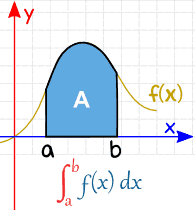
\includegraphics{./lect1/pic1.png}
\end{center}
$$f:[a,b] \to R$$
$$m \leq f(x) \leq M \quad \forall a \leq x \leq b$$
It's obvious that $m(b-a) \leq S\leq M(b-a)$. Define partition $P$ of $[a,b]$:
$$a=x_0<x_1<\dots<x_n=b$$
Given partition $P$ denote 
$$m_i := \inf f(x) [x_{i-1} x_{i}]$$

$$M_i := \sup f(x) [x_{i-1} x_{i}]$$
$$\Delta x_i = x_i - x_{i-1}$$

\begin{center}
	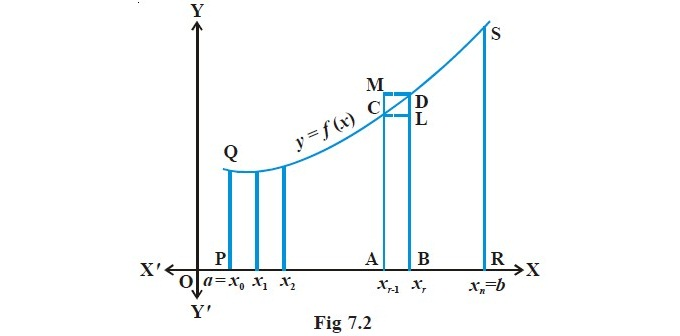
\includegraphics{./lect1/pic2.jpg}
\end{center}
For each of intervals $[x_{i-1}, x_i]$ the area under the graph is $m_i\Delta x_i \leq S_i \leq M_i \Delta x_i$. Then for the total area, due to property 2, we want
$$\sum_{i=1}^n m_i \Delta x_i \leq S \leq \sum_{i=1}^n M-i \Delta x_i$$

Denote:
$$U(P,f) = \sum_{i=1}^n M_i \Delta x_i$$
$$L(P,F) = \sum_{i=1}^n m_i \Delta x_i$$
which are called upper and lower Darboux sums.
$$\forall P \quad L(P,f) \leq S \leq U(P,f)$$

\paragraph{Refinements} Let $P$, $P^\prime$ two partitions of $[a,b]$. $P^\prime$ refines $P$ if each point in $P$ is also in $P^\prime$. 
\paragraph{Claim} $U(P^\prime) \leq U(P)$ and $L(P^\prime) \geq L(P)$.
\subparagraph{Proof} 
$$P:\: a=x_0<x_1<\dots<x_n=b$$
$$P^\prime:\: a=x_0<x_1<\dots x_k<x^\prime < x_{k+1}< \dots<x_n=b$$
Denote $M^\prime = \sup f [x_k, x^\prime]$ and $M^{\prime \prime} = \sup f [x^\prime, x_k+1]$.
Then $U(P^\prime) = M_1 \Delta x_1 + \dots + M_K \Delta x_k + M^\prime \left( x^\prime - x_k \right) + M^{\prime \prime} \left( x_{k+1} - x^\prime \right) + \dots$
$$U(P^\prime)-U(P) = M^\prime \left( x^\prime - x_k \right) + M^{\prime \prime} \left( x_{k+1} - x^\prime \right) - M_{k+1} \left( x_{k+1} - x_k \right)$$
But $M^\prime, M^{\prime \prime} \leq M_{k+1}$
$$U(P^\prime)-U(P) \leq M_{k+1} \left(x_{k+1} - x_k\right) -  M_{k+1} \left(x_{k+1} - x_k\right) = 0$$

\paragraph{} Denote parameter of partition $\lambda(P) = \max_i \Delta x_i$
\paragraph{Note} Given two partitions $P, P^\prime$ exists partition $P^{\prime \prime}$ which includes both of them (acquired by union)
\paragraph{Conclusion} For any two partitions $P$, $P^\prime$ $L(P) \leq U(P^\prime)$
\subparagraph{Proof} Let $P^{\prime \prime}$ mutual refinement of $P$ and $P^\prime$. Then
$$L(P) \leq L(P^{\prime \prime}) \leq U(P^{\prime \prime}) \leq U(P^\prime)$$
\paragraph{Conclusion} $\sup L(P) \leq \inf (U(P))$.
\paragraph{Definition} Let $f$ bounded on $[a,b]$. We say that $f$ is Riemann integrable if $\sup L(P) = \inf (U(P))$. In this case we denote this value $\int_a^b f(x) dx$ and call it definite integral of $f$ on $[a,b]$. If this integral exists we can think on it as area under $f$ on $[a,b]$.

When $f(t)$ denotes temp of change then $\int_a^b f(t) dt$ denotes total change.
\subsection{Examples}
\paragraph{} 
$$
D(x) = \begin{cases}
0&x\in\mathbb{Q}\\
1&x\notin\mathbb{Q}\\
\end{cases}
$$
For any partition $L(P,D) = 0$ and $U(P,D) = 1 \Rightarrow$ $D$ isn't integrable.
\paragraph{} $f(x) = c$ on $[a,b]$. Then $M_i = m_i = c$. By definition $$\int_a^b c dx= c(b-a)$$ 
\paragraph{} $f(x) =x$ on [0,1]. Define $P_n: 0 < \frac{1}{n}  < \frac{2}{n} < \dots < \frac{n-1}{n} < 1$. Then
$$U(P_n,f) = \frac{1}{n} \cdot \frac{1}{n} +  \frac{2}{n} \cdot \frac{1}{n} + \dots +  1 \cdot \frac{1}{n} = \frac{1}{n^2} \cdot \sum_{k=1}^{n} k = \frac{1}{n^2} \cdot \frac{n(n+1)}{2}  = \frac{1}{2} \left( 1+ \frac{1}{n} \right)$$ 
Similarly
$$L(P_n,f) = \frac{1}{n^2} \cdot \sum_{k=1}^{n} \left(k-1\right) = \frac{1}{2} \left( 1+- \frac{1}{n} \right)$$ 
Then $\inf U(P_n, f) = \sup L(P_n,f) = \frac{1}{2}$. However, those are not all partitions. But
$$\frac{1}{2} \leq \sup L(P,f) \leq \inf U(P,f) \leq \frac{1}{2}$$
meaning $f(x)$ is integrable and $\int_0^1 x dx =\frac{1}{2}$.
\paragraph{Theorem} Given $P\subseteq P^\prime$, suppose $P^\prime$ is refinement of $P$ acquired by adding $q$ points. Then $0 \leq U(P) - U(P^\prime) \leq \lambda(P)\cdot q \cdot (M-m)$ and $0 \leq L(P^\prime) - L(P) \leq \lambda(P)\cdot q \cdot (M-m)$.
\subparagraph{Proof} With previous symbols, i.e 
$$P:\: a=x_0<x_1<\dots<x_n=b$$
$$P^\prime:\: a=x_0<x_1<\dots x_k<x^\prime < x_{k+1}< \dots<x_n=b$$
$M^\prime = \sup f [x_k, x^\prime]$ and $M^{\prime \prime} = \sup f [x^\prime, x_k+1]$.

Suppose $q=1$ (it's enough), then
\begin{align*}
U(P) - U(P^\prime) = M_{k+1} \underbrace{\left( x_{k+1} - x_k \right)}_{x_{k+1}-x^\prime + x^\prime - x_k} - M^\prime \left( x^\prime - x_k \right) - M^{\prime \prime} \left( x_{k+1} - x^\prime \right) = \left(M_{k+1} - M^\prime\right)\left( x^\prime - x_k \right) +  \left(M_{k+1} - M^{\prime\prime}\right)\left( x_{k+1} - x^\prime \right) \leq\\
\leq (M-m)(x^\prime-x_k)+(M-m)(x_{k+1}-x^\prime) = (M-m)(x^\prime - x_k + x_{k+1}-x^\prime) = (M-m)\Delta x_{k+1} \leq (M-m) \cdot \lambda(P)
\end{align*}
\paragraph{Theorem} Following conditions are equivalent for bounded $f(x)$:
\begin{enumerate}
	\item $f(x)$ is integrable
	\item $\forall \epsilon > 0 \: \exists P_\epsilon$ such that $U(P_\epsilon) - L(P_\epsilon) < \epsilon$. Denote $W(P_\epsilon, f) = U(P_\epsilon) - L(P_\epsilon) = \sum \left(M_i - m_i\right) \cdot \Delta x_i$
	\item $\forall \epsilon > 0 \: \exists \delta > 0 $ such that if $\lambda(P) < \delta$ for some $P$, then $W(P) < \epsilon$.
\end{enumerate}
\subparagraph{Proof} Obviously, $3 \Rightarrow 2$.

If 2 is right, then $\inf U(P) - \sup L(P) \leq U(P_\epsilon) - L(P_\epsilon) < \epsilon \quad \forall \epsilon > )$, i.e. $\inf U(P) - \sup L(P) = 0$.

Now let's proof $1 \Rightarrow 3$. Suppose $f(x)$ is integrable and denote $I = \int_a^b f(x) dx$. Let $\epsilon > 0$ then exists $P^\prime$ such that $I \leq U(P^\prime) \leq I + \frac{\epsilon}{4}$ (since $I$ is infimum). 

Let's choose $\delta = \frac{\epsilon}{4n(M-m)}$ when $n$ is number of points in $P^\prime$. (if $M=m$ then proof is trivial).

We choose $P$ such that $\lambda(P) < \delta$ and $P^{\prime\prime}$ is union of points of $P$ and $P^\prime$. Suppose there are $p$ more points in $P^{\prime\prime}$ than in $P$. Note that $p \leq n$. Then
$$I \leq U(P) \leq U(P^{\prime \prime}) + \lambda(P)\cdot p\cdot(M-m) \leq U(P^{\prime \prime}) + \lambda(P) \cdot n \cdot (M-m) \stackrel{\scriptsize \delta = \frac{\epsilon}{4n(M-m)}}{\leq} U(P^{\prime \prime})  + \frac{\epsilon}{4} \leq U(P^\prime)  + \frac{\epsilon}{4} \leq I + \frac{\epsilon}{2} $$
which means $I \leq U(P) \leq I+\frac{\epsilon}{2}$. Similarly we can get $I \geq L(P) \geq I-\frac{\epsilon}{2}$, i.e. $W(P) < \epsilon$
	\paragraph{Theorem} If $f$ is monotonic on $[a,b]$ than it's integrable.
\subparagraph{Proof} Suppose without loss of generality that $f$ is non-decreasing.
It's obvious that $f$ in bounded: $\forall x \: f(a)\leq f(x) \leq f(b)$.

For partition $P$, $m_i = f(x_{i-1})$ and $M_i = f(x_i)$.

$$W(P) = U(P,f) - L(P,f) = \sum \left( f(x_i) - f(x_{i-1}) \right) \Delta x_i $$

For $\epsilon > 0$ lets take $\delta = \frac{\epsilon}{f(b)-f(a)}$.

If $\delta > \lambda(P) \Rightarrow \forall \Delta x_i <  \frac{\epsilon}{f(b)-f(a)}$ and 
$$W(P) \leq \frac{\epsilon}{f(b)-f(a)} \sum \left( f(x_i) - f(x_{i-1}) \right) = \frac{\epsilon}{f(b)-f(a)}  \cdot \left(f(b)-f(a)\right) = \epsilon$$
Meaning $f$ is integrable.
\paragraph{Theorem} If $f$ is continuous on $[a,b]$ than it's integrable.
\subparagraph{Proof} Since $f$ is continuous on a closed interval it's uniformly continuous $\Rightarrow \forall \epsilon > 0 \exists \delta > 0 $ such that if $|x-y| < \delta$ then $|f(x)-f(y)| < \epsilon$.

Lets choose $\epsilon > 0 $ and $\delta > 0 $ such that if $\delta > |x-y| \Rightarrow \frac{\epsilon}{b-a} > |f(x)-f(y)|$.

Suppose $P$ partition with $\lambda(P) < \delta$
From uniform continuousness $\forall i M_i-m_i \leq \frac{\epsilon}{b-a}$ then $$U(P)-L(P) = \sum (M_i-m_i) \Delta x_i \leq \frac{\epsilon}{b-a} \sum \Delta x_i = \epsilon$$

\paragraph{Theorem} If $f$ is continuous on $[a,b]$  except finite number of points  than it's integrable.
\subparagraph{Proof} 
Let $\epsilon > 0$. Suppose $f(x)$ has $k$ non-continuous points. Choose $\delta_1 = \frac{\epsilon}{8(M-m)k}$.

Denote $A = [a,b] \setminus \bigcup (t_i-\delta_1, t_I+\delta_1)$, where $t_1 \dots t_i$ - points of non-continuousness.

$A$ is finite union of closed intervals and $f$ is continuous on each of them. Exists $\delta_2 > 0$ such that if $|x-y| < \delta_2$ and $[x,y] \in A$ then $|f(x)-f(y)| < \frac{\epsilon}{2(b-a)}$. Denote $\delta = min(\delta_1, \delta_2)$ and let $P$ is partition such that $\lambda(P) < \delta$.
$$U(P)-L(P) = \sum_{i=1}^{n} (M_i-m_i) \Delta x_i = \sum^\prime \parbox{2cm}{\centering \scriptsize intervals contained in A} +  \sum^{\prime\prime} \parbox{2cm}{\centering \scriptsize intervals non contained in A} $$
Lets approximate both sums. First one is simple:
$$\sum^\prime \stackrel{\scriptsize M_i-m_i \leq \frac{\epsilon}{2(b-a)}}{\leq} \frac{\epsilon}{2(b-a)}(b-a) = \frac{\epsilon}{2}$$
For the second one, total length of all intervals around each non-continuous point is less than $4\delta_1$:
$$\sum^{\prime\prime} \leq (M_i-m_i)\sum^{\prime\prime} \Delta x_i < (M_i-m_i) \cdot 4\delta_1 k = \frac{\epsilon}{2}$$
Then 
$$U(P)-L(P) < \epsilon$$
\paragraph{Examples}
$$f(x) = \begin{cases}
\sin^2(1/x)&x\leq=0\\ 0&x=0
\end{cases}$$
is integrable on $[-1,1]$.
$$f(x) = \begin{cases}
1-\frac{1}{2^{n-1}}&\frac{1}{2^{n-1}}\leq x < \frac{1}{2^{n}}\\1&x=1
\end{cases}$$
is integrable since it's monotonic.
	\subsection{Riemann sums}
Given partition $P$ and points $\left\{t_i\right\}_{i=1}^n$ such that $x_{i-1} \leq t_I \leq x_i$, Riemann sum is
$$\sigma\left(P,f,\left\{t_i\right\}\right) = \sum_{i=1}^n f(t_i) \Delta x_i$$
If $f$ is bounded, $$L(P,f)\leq \sigma\left(P,f,\left\{t_i\right\}\right) \leq U(P,f)$$
\paragraph{Theorem} Let $f$ defined on $[a,b]$. It is integrable iff exists $I$ such that $\forall \epsilon > 0 \exists \delta > 0 $ such that for any partition $P$ that upholds $\lambda(P) < \delta$ and for any choice of points $$\left| \sigma\left(P,f,\left\{t_i\right\}\right) - I \right| < \epsilon $$
In this case $I  = \int_a^b f(x) $ and it's the only number upholding the condition.
\subparagraph{Proof}
Suppose $f$ integrable (and then it's bounded). Let $\epsilon > 0$ then $\exists \delta > 0$ such that $\forall \lambda(P) < \delta$, $0 \leq U(P) - L(P) < \epsilon$. Let $\left\{t_i\right\}$ choice of points. Since $$L(P) \leq \int_a^b f(x)  \leq U(P)$$ and $$L(P) \leq \sigma\left(P,f,\left\{t_i\right\}\right) \leq U(P)$$
$$\left| \sigma\left(P,f,\left\{t_i\right\}\right) -  \int_a^b f(x)  \right| \leq U(P) - L(P) < \epsilon$$
This means that $\int_a^b f(x)  $ upholds the condition of I.
Uniqueness: if $I^\prime$ also upholds the condition ($\left| \sigma\left(P,f,\left\{t_i\right\}\right) - I^\prime \right| < \epsilon $), then $I-I^\prime < \epsilon$, i.e. $I=I^\prime$.

Now suppose exists $I$ that upholds the condition. First proof $f$ is bounded, so that Darboux sums exist.

Take $\epsilon=1$ and $\delta > 0 $. Suppose $f$ isn't bounded and choose $P$ such that $\lambda(P) < \delta$. Exists $i$ such that $f$ isn't bounded on $\left[x_{i-1}, x_i\right]$. Lets choose $\left\{t_i\right\} \: j \neq i$. At interval $\left[x_{i-1}, x_i\right]$ we choose point $t$. Since $$\sigma\left(P,f,\left\{ t_j \right\}\right) < 1$$
$$\sum_j f(t_j) \Delta x_j - I < 1$$
$$\sum_{j\neq i} f(t_j) \Delta x_j + f(t) \Delta x_i < I + 1$$
We can choose a sequence of $t$ such that $f(t_m) \to \infty$ and it's contradiction.

Let $\epsilon > 0$ and $\delta > 0$ according to condition and $P$ is partition with $\lambda(P) < \delta$. Lets choose points $t_i$, $s_i$ such that 
$$\left|f(s_i) - M_i\right| < \frac{\epsilon}{2(b-a)}$$
$$\left|f(t_i) - m_i\right| < \frac{\epsilon}{2(b-a)}$$
Then
$$0 \leq \sigma\left( P, f, \left\{t_i \right\} \right) - L(P,f) < \frac{\epsilon}{2(b-a)} \cdot \sum \Delta x_i = \frac{\epsilon}{2}$$
$$0 \leq U(P,f) - \sigma\left( P, f, \left\{t_i \right\} \right)  < \frac{\epsilon}{2}$$
and also
$$\left| \sigma\left(P,f,\left\{t_i\right\}\right) -  \int_a^b f(x)  \right|  < \epsilon$$
$$\left| \sigma\left(P,f,\left\{s_i\right\}\right) -  \int_a^b f(x)  \right|  < \epsilon$$
Then
$$U(P,f)-L(P,f) < 3 \epsilon$$

\paragraph{Theorem} Let f,g integrable on $[a,b]$ then
\begin{enumerate}
	\item $f+g$ integrable and $\int_a^b (f+g)  = \int_a^b f +\int_a^b g $
	\item $cf$ is integrable of $c \in \mathbb{R}$ and $\int_a^b cf  = c\int_a^b f $
	\item If $f \leq g$ on $[a,b]$ then $\int_a^b f  \leq \int_a^b g $
\end{enumerate}
\subparagraph{Proof} 
Note: the theorem is right since 1-3 is right for Riemann sums.

From previous theorem, given $\epsilon > 0$ exists $\delta > 0$ such that for any partition $\lambda(P) < \delta$ and for any choice of points $\left\{ t_i \right\}$
$$\int_a^b f  - \sigma \left(P,f, \left\{ t_i \right\} \right) < \frac{\epsilon}{2}$$
$$\int_a^b g  - \sigma \left(P,g, \left\{ t_i \right\} \right) < \frac{\epsilon}{2}$$
Then
$$\left| \int_a^b (f+g)  - \sigma \left(P,f+g, \left\{ t_i \right\}\right) \right| = \left| \int_a^b f  + \int_a^b g  - \sigma \left(P,f, \left\{ t_i \right\}\right) - \sigma \left(P,g, \left\{ t_i \right\}\right) \right| < \epsilon $$
\paragraph{Theorem}
\begin{enumerate}
	\item If $f$ integrable on $[a,b]$, then it's integrable on each subinterval $[\alpha, \beta] \subseteq [a,b]$.
\item If $a<c<b$ and $f$ integrable on $[a,c]$ and $[c,b]$ then $f$ is integrable on $[a,b]$ and $\int_a^b f  = \int_a^c f  + \int_c^b f $.
\end{enumerate}
\subparagraph{Proof}
\begin{enumerate}
	\item Let $\epsilon > 0$, exists partition $Q$ of $[a,b]$ such that $W(Q,f) < \epsilon$. Let $P$ partition that refines $Q$ by addition of $\alpha$ and $\beta$, then $W(P,f) \leq W(Q,f)$.

Let $P^\prime$ partition of $[\alpha, \beta]$ which is acquired from points of $P$  which are contained in $[\alpha, \beta]$. Then $W(P^\prime, f) \leq W(P,f) < \epsilon$ 
\item Suppose that $f$ is integrable on $a,c$ and $[c,b]$. For $\epsilon > 0$ exists $\delta > 0 $ such that for any $\lambda(P_1) < \delta$ partition of $[a,c]$ and choice of points $ \left\{ t_i \right\}$
$$\left| \int_a^c f - \sigma (P_1, f, \left\{ t_i \right\}) \right| < \frac{\epsilon}{3}$$
Similarly, for $[c,b]$
$$\left| \int_c^b f - \sigma (P_2, f, \left\{ s_i \right\}) \right| < \frac{\epsilon}{3}$$

Now lets take partition $P$ of $[a,b]$ with $\lambda(P)<\delta$. Refine it with addition of $c$ and acqire $P_c$ and choose points $ \left\{ z_i \right\}$ for it.	
Then

$$\sigma\left( P_c, f,  \left\{ z_i \right\} \right) = \sum_{i=1}^n f(z_i) \Delta x_i = \sum_{i=1}^k f(z_i) \Delta x_i + \sum_{i=k+1}^n f(z_i) \Delta x_i = \sigma\left( P_1, f,  \left\{ z_i \right\}_1^k \right) + \sigma\left( P_2, f,  \left\{ z_i \right\}_{k+1}^n \right)$$
Since
$$\left|\int_a^c f - \sigma\left( P_1, f,  \left\{ z_i \right\}_1^k \right) \right|< \frac{\epsilon}{3}$$
$$\left|\int_c^b f - \sigma\left( P_2, f,  \left\{ z_i \right\}_{k+1}^n \right) \right| < \frac{\epsilon}{3}$$
we get
$$\left|\sigma\left( P_c, f,  \left\{ z_i \right\} \right) - \int_a^c f - \int_c^b f \right| < \frac{2\epsilon}{3}$$
Returning to partition $P$, suppose $c < z_k < x_k$ and $P_c$ partition including $c$. Lets take same points $z_k$ for both, but at $x_{k-1}, c$ we choose $c$ as a point for $P_c$. Then
\begin{align*}
\bigg|\sigma\left( P_c, f,  \left\{ z_i \right\} \right) - \sigma\left( P, f,  \left\{ z_i \right\} \right) \bigg| = \bigg| \underbrace{(c-x_{k-1})f(c) + (x_k - c )f(z_k) }_{P_c} -\underbrace{ (x_k-x_{k-1})f(z_k)}_{P} \bigg| =\\= \bigg| \underbrace{(f(c) - f(z_k))}_{<M-m}\underbrace{(c-x_{k-1})}_{<\delta} \bigg| < \delta (M-m) < \frac{\epsilon}{3}
\end{align*} 
Which means
$$\left|\sigma\left( P, f,  \left\{ z_i \right\} \right) - \int_a^c f - \int_c^b f \right| < \epsilon$$
\end{enumerate}
	
	\section{Connection between definite integral and antiderivative}
Let function integrable Riemann on $[a,b]$ and $F(x) = \int_a^b f(t) dt$
\paragraph{Theorem} F is continuous on $[a,b]$
\paragraph{Theorem} Let $f$ integrable on $[a,b]$ and continuous in $x_0 \in [a,b]$ then $F$ is derivable in $x_0$ and $F^\prime(x_0) = f(x_0)$. If $x_0$ is one of endpoints, derivative will be one-sided.
\subparagraph{Proof}
Suppose $x_0 \in [a,b)$. For all $b>x>x_0$ $$F(x)-F(x_0) = \int_a^x-f dt - \int_a^{x_0} f dt = \int_{x_0} f(t) dt$$
$f$ is continuous in $x_0$: for any $\epsilon > 0$ exists $\delta > 0$ such that if $|x-x_0| < \delta$ $|f(x)-f(x_0)| < \epsilon$. That means 
$$f(x_0) - \epsilon < f(x) < f(x_0) + \epsilon$$
From monotonousness of integral:
$$(f(x_0)-\epsilon)(x-x_0) = \int_{x_0}^x (f(t)-\epsilon) dt \leq \underbrace{\int_{x_0}^x f(t) dt}_{F(x)-F(x_0)} \leq \int_{x_0}^x (f(t) +\epsilon) dt = (f(x)+\epsilon)(x-x_0)$$ 
Suppose $x>x_0$
$$f(x_0) -\epsilon \leq \frac{F(x)-F(x_0)}{x-x_0} \leq f(x_0)+ \epsilon$$
That means that for any $\epsilon > 0$ exists $\delta > 0$ such that if $x_0+\delta > x > x_0$ then
$$f(x_0) -\epsilon \leq \frac{F(x)-F(x_0)}{x-x_0} \leq f(x_0)+ \epsilon$$
$$\lim_{x\to x_0^+} \frac{F(x)-F(x_0)}{x-x_0} = f(x_0)$$
In a similar way we can show that for $x \in (a,b]$
$$\lim_{x\to x_0^-} \frac{F(x)-F(x_0)}{x-x_0} = f(x_0)$$
It means for $x \in (a,b)$
$$F^\prime(x_0) = \lim_{x\to x_0}\frac{F(x)-F(x_0)}{x-x_0} = f(x_0)$$
\paragraph{Conclusion}
If $f$ is continuous on $[a,b]$ then $F$ is derivable there and $$F^\prime(x) = f(x)$$
\paragraph{Reminder} Antiderivative, if exists, is unique.
\paragraph{Theorem} If $f$ is continuous on $[a,b]$ and $G$ is antiderivative of $f$, then $$\int_a^b f(t) dt = G(b) -G(a)$$
\subparagraph{Proof}
$$\int_a^b f(t) dt =F(b) - F(a) = G(b) -G(a)$$
\subsection{Integration by parts}
$$\int uv^\prime dx = uv - \int vu^\prime dx$$
$$\int_a^b uv^\prime dx = \left[ uv - \int vu^\prime dx \right]_a^b = \left[ uv \right]_a^b - \int_a^b vu^\prime dx$$
\paragraph{Example}
$$\int_1^e x \ln x dx = \left[\frac{x^2 \ln x}{2}\right]_1^e - \int_1^e \frac{x^2}{2}\cdot \frac{1}{x} dx = \frac{1}{2}e^2 - 0 - \left[ \frac{1}{4}x^2 \right]_1^e = \frac{1}{2}e^2 - \frac{1}{4}e^2 + \frac{1}{4} = \frac{1}{4} \left( e^2 + 1 \right) $$
\subsection{Integration by substitution}
Suppose $F^\prime = f $ and $g$ derivable function such that $f\circ g$ and $F \circ g$ are defined. Then
$$\int f(g(x)) g^\prime(x) dx = F(g(x)) + C$$
\paragraph{Definite integral}
Suppose $g$ is defined and continuously derivable on $I$. Let $f$ continuous on $I$   with antiderivative $F$ . Then
$$\int_a^b f(g(x)) g^\prime(x) dx = \left[ F(g(x))\right]_a^b = \int_{g(a)}^{g(b)} f(t) dt$$ 
\paragraph{Example}
$$\int_0^{\frac{\pi}{2}} \sin^2 x \cos x dx =\left[ \frac{1}{3} \sin^3 x\right]_0^{\frac{\pi}{2}} = \int_0^1 t^2 dt = \left[ \frac{1}{3} y^3 \right]_0^1 = \frac{1}{3}$$
$g(x) = \sin x$, $f(x) = x^2$, $F(x) = \frac{1}{3} x^3$
\section{Improper integrals}
Until now we discussed only integrals of bounded functions on finite intervals. What happens with unbounded functions or on infinite interval?
\paragraph{Interval $[a, \infty)$}
Let f defined on $[a,\infty)$ and integrable on $[a,c]$ for any $c>a$. we say that improper integral of $f$ exists (or $f$ integrable on  $[a,\infty)$) if $$\lim_{c\to \infty} \int_a^c f(x) dx$$ exists and finite. At this case we denote $$\int_a^\infty f(x) dx = \lim_{c\to \infty} \int_a^c f(x) dx$$
\paragraph{Example}
$f(x) = \frac{1}{x^\alpha}$, $\alpha \in \mathbb{R}$ on $[1, \infty)$.
$$\int_1^\infty \frac{1}{x^\alpha} dx = ?$$
\subparagraph{Solution}
$$\int_1^\infty \frac{1}{x^\alpha} dx = \begin{cases}
[\ln x]_1^c = \ln c &\alpha = 1 \\
\left[\frac{1}{(1-\alpha)}x^{1-\alpha}\right]_1^c = \frac{1}{(1-\alpha)}\left(c^{1-\alpha}-1\right) & \alpha \neq 1
\end{cases}$$
If $\alpha = 1$, since $\lim_{x \to infty} \ln x  = \infty$, integral doesn't exists.
Similarly, it doesn't exists if $\alpha < 1$.
If $\alpha > 1$
$$\lim_{c \to \infty} \int_1^c \frac{1}{x^\alpha} dx = - \frac{1}{1-\alpha} = \frac{1}{\alpha - 1}$$
That means that
$$\int_1^\infty \frac{1}{x^\alpha} dx = \frac{1}{\alpha -1}$$
\paragraph{Example}
$$\int_0^\infty \sin x dx = \lim_{c \to \infty} \int_0^c \sin x dx = \lim_{c \to \infty} \left[-\cos x \right]_0^c =  \lim_{c \to \infty} \left( \cos c + 1 \right)$$
limit doesn't exist.

\paragraph{Interval $(-\infty,a]$}

Let f defined on $(-\infty,a]$ and integrable on $[c,a]$ for any $c<a$. we say that improper integral of $f$ exists (or $f$ integrable on  $(-\infty,a]$) if $$\lim_{c\to -\infty} \int_c^a f(x) dx$$ exists and finite. At this case we denote $$\int_{-\infty}^a f(x) dx = \lim_{c\to -\infty} \int_c^a f(x) dx$$
\paragraph{Example}
$$\int_{-\infty}^{0} e^x dx = \lim_{c \to -\infty} \int_{c}^{0} e^x dx = \lim_{c \to -\infty}  \left[ e^x \right]_c^0 = \lim_{c \to -\infty}  1 - e^c = 1$$


\paragraph{Interval $(-\infty,\infty)$}

$\int_{-\infty}^{\infty} f(x) dx$ exists if both $\int_{a}^{\infty} f(x) dx$  and $\int_{-\infty}^{a} f(x) dx$  exist for some a. In this case
$$\int_{-\infty}^{\infty} f(x) dx = \int_{a}^{\infty} f(x) dx + \int_{-\infty}^{a} f(x) dx$$
\paragraph{Example}
$$\int_{-\infty}^{\infty}  \sin x dx$$
doesn't exist, as shown earlier.

However, if we'd take $$\lim_{c\to \infty} \int_{-c}^{c} \sin x dx = \lim_{c\to \infty} -\cos c + \cos (-c) = 0$$
$\lim_{c\to \infty} \int_{-c}^{c} f(x) dx$, if exists, is called principal value.
\paragraph{Unbounded function}
Let $f$ defined on $[a,b)$ and integrable on $[a,c]$ for all $a<c<b$. We say that $f$ is integrable on $[a,b)$ if $\lim_{c\to b} \int_a^c f(x) dx $ exists and finite. We denote
$$\int_a^b f(x) dx = \lim_{c\to b} \int_a^c f(x) dx$$

Similarly, let $f$ defined on $(a,b]$ and integrable on $[c,b]$ for all $a<c<b$. We say that $f$ is integrable on $(a,b]$ if $\lim_{c\to a} \int_c^b f(x) dx $ exists and finite. We denote
$$\int_a^b f(x) dx = \lim_{c\to a} \int_c^b f(x) dx$$
\paragraph{Exercise} Let $f$ bounded on $[a,b]$ and integrable on $[a,c]$ for all $a<c<b$. Proof that $f$ is integrable on $[a,b]$ and $$\int_a^b f(x) dx= \lim_{c\to b} \int_a^c f(x) dx$$
\paragraph{Example}
$$\int_0^1 \frac{1}{x^\alpha}dx$$
$$\int_c^1 \frac{1}{x^\alpha}dx = \begin{cases}
\left[\ln x\right]_0^1 = -\ln c & \alpha = 1 \\
\frac{1}{1-\alpha}\cdot (1-c^{1-\alpha})&\alpha \neq 1
\end{cases} $$
Integral exists only if $\alpha <1$.
	\paragraph{Example}
If we have more than one ``problem'', we divide integral into two, one for each problem. For example:
$$\int_0^\infty \frac{1}{x^\alpha} dx$$
This particular integral doesn't exist for any $\alpha$.
\paragraph{Example}
$$\int_0^6 \frac{1}{\left(x-2\right)^2}dx$$
We might use the fact that antiderivative is $$\left[-\frac{1}{x-2}\right]_0^6 = -\frac{1}{4}-\frac{1}{2}=-\frac{3}{4}$$
However, this isn't right, since function isn't integrable (not bounded). Instead, we should divide the problem into two improper integrals:
$$\int_0^6  \frac{1}{\left(x-2\right)^2}dx = \int_0^2  \frac{1}{\left(x-2\right)^2}dx + \int_2^6  \frac{1}{\left(x-2\right)^2}dx$$
$$\int_0^2  \frac{1}{\left(x-2\right)^2}dx  = \lim_{c \to 2^-}\int_0^c  \frac{1}{\left(x-2\right)^2}dx = \left[-\frac{1}{x-2}\right]_0^c =  \lim_{c \to 2^-} -\frac{1}{c-2} - \frac{1}{2} = -\infty$$
which means the integral doesn't exists.
\paragraph{Claim}
If $f$,$g$ integrable on $[a,\infty)$ then both $f+g$ and $c\cdot g$ are integrable on $[a,b]$ and
$$\int_a^\infty (cf+g) = c\int_0^\infty f + \int_0^\infty g$$
\subparagraph{Proof} is trivial, from linearity of the integral. This is right for all other types of improper integrals.
\paragraph{Theorem} Let f defined on $[a, \infty)$ and integrable on every $[a,c]$ for $c>a$. Then $\int_a^\infty f dx$ exists if $\forall \epsilon > 0 \exists M$ such that if $c_2\geq c_1 \geq M$ then $\left| \int_{c_1}^{c_2} \right| < \epsilon$
\subparagraph{Proof} $\lim_{x\to \infty} F(x) \iff \forall \epsilon > 0  \exists M$ such that if $c_2\geq c_1 \geq M$ then $\left| F(c_2)-F(c_1) \right| < \epsilon$ when $F(x) = \int_a^x f dx$ 
\paragraph{Theorem} Let f defined on $[a, b)$ and integrable on every $[a,c]$ for $b>c>a$. Then $\int_a^b f dx$ exists if $\forall \epsilon > 0 \exists \delta > 0$ such that if $b>c_2\geq c_1 > b -\delta$ then $\left| \int_{c_1}^{c_2} \right| < \epsilon$
\paragraph{Conclusion}Let $f$ defined on $[a, \infty)$ and integrable on every $[a,c]$ for $c>a$. If exists $\int_a^\infty \left| f \right| dx $ the also $\int_a^\infty f dx$ exists.
\subparagraph{Proof} Using $$\left| \int_{c_1}^{c_2} f dx \right| \leq \int_{c_1}^{c_2} \left|  f dx \right| < \epsilon $$
\paragraph{Definition} If exists $\int_a^\infty |f| dx$ we tell that integral converges absolutely. According to conclusion, if integral converges absolutely, it converges.
\paragraph{Example} Note that conclusion has other conditions:
$$g(x)  =\begin{cases}
1&x\in \mathbb{Q}\\
-1&x\in \mathbb{Q}\\
\end{cases}$$
$g(x)$ isn't integrable, but $|g(x)|$ is.
\subsection{Existence of improper integral for $f\geq0$}
\paragraph{Theorem} $f\geq 0$ on $[a, \infty)$ integrable on every $[a,c]$ for $c>a$ and $F(x) = \int_a^x f dt$. Then $\int_a^\infty f dx$ exists $\iff F$ is bounded.
\subparagraph{Proof} $F$ is monotonous: $x_1 > x_2  \Rightarrow F(x_1) = \int_a^{x_1} = \int_a^{x_2} + \int_{x_2}^{x_1} \geq \int_a^{x_2} = F(x_2)$.

That means that $\lim_{c\to \infty} F(c)$ exists iff $F(x)$ is bounded.
\paragraph{Theorem} Let $k>0$ and $f,g$ that are defined  on $[a, \infty)$ integrable on every $[a,c]$ for $c>a$ and $\forall x>a \:0 \leq f(x) \leq kg(x)$. If $\int_a^\infty g(x)$ exists, then also $\int_a^\infty f(x)$ exists.
\subparagraph{Proof} Denote $F(x)=\int_a^x f(t) dt$ and $G(x)=\int_a^x g(t) dt$. From monotonousness of integral, $F(x) \leq kG(x)$. Since $G(x)$ is bounded, $F(x)$ is bounded too, meaning $f(x)$ is integrable.
\subparagraph{Note} It's enough that $\leq f(x) \leq kg(x)$ just for $x>c$ for some c.
\paragraph{Example}
$$\int_1^\infty \frac{\sin x}{x^2} dx $$
To use previous theorems, we take the absolute value: $$\left| \frac{\sin x}{x^2} \right| \leq \frac{1}{x^2}$$ Since $\frac{1}{x^2}$ is integrable, $\left| \frac{\sin x}{x^2} \right|$ is integrable too, and therefore, $\frac{\sin x}{x^2}$ converges.
\paragraph{Example}

$$\int_1^\infty \frac{\sin x}{x} dx = \lim_{c\to \infty} \int_1^c \frac{\sin x}{x} dx $$
Integrating by parts:
$$\int_1^c \frac{\sin x}{x} dx  = \left[-\frac{\cos x}{x}\right]_1^c - \underbrace{\int_1^c \frac{\cos x}{x^2} dx}_{\parbox{1cm}{\scriptsize \centering exists}}$$
$$\lim_{c \to \infty} \left[-\frac{\cos x}{x}\right]_1^c = \lim_{c \to \infty} -\frac{\cos c}{c} + \cos 1 = \cos 1$$
Since limit exists, integral converges.
\paragraph{Example}
$$\int_1^\infty \left|\frac{\sin x}{x}\right| dx$$ doesn't exist. First, lets show that $$\int_1^\infty \frac{\sin^2 x}{x} dx$$ doesn't exists.
First of all, $$\int_1^c \frac{\sin^2 x}{x} = \int_1^c \frac{1}{2x} - \int_1^c \frac{\cos 2x}{2x}$$
$ \int_1^c \frac{1}{2x} = \left[\ln x\right]_1^c$ which diverges. Back to $\left|\frac{\sin x}{x}\right|$, since   $\frac{\sin^2 x}{x}<\left|\frac{\sin x}{x}\right|$, $\int_1^\infty \left|\frac{\sin x}{x}\right|$ doesn't exists.
\paragraph{Theorem} For two functions $f,g \geq 0$ integrable on every $[a,c]$. Suppose $$\lim_{x \to \infty} \frac{f(x)}{g(x)} = L$$ and $0 < L < \infty$. Then $\int_a^\infty f(x)$ converges iff $\int_a^\infty g(x)$ converges.
\subparagraph{Proof} $\lim \frac{f}{g} = L$ which means that exists $n$ such that for all $x>n$ $$\frac{L}{2} < \frac{f(x)}{g(x)} < 2L$$
$$f(x) < 2Lg(x)$$
$$\frac{2}{L}f(x) > g(x)$$
From comparison theorem  $\int_a^\infty f(x)$ converges iff $\int_a^\infty g(x)$ converges.
\paragraph{Example}
$$\int_1^\infty \sin \frac{1}{x}dx$$
Compare with $\frac{1}{x}$:
$$\lim_{x\to\infty} \frac{\sin\frac{1}{x}}{\frac{1}{x}} = 1$$
Since $\int_1^\infty \frac{1}{x}$ doesn't exists, $\int_1^\infty \sin \frac{1}{x}dx$ doesn't exist too.
\paragraph{Example}
$$\int_0^\infty \frac{\sqrt{x}}{\sqrt{1+x^4}}$$
exists, since $f(x) \propto x^{-\frac{3}{2}}$.
\paragraph{Dirichlet's theorem} Let $f(x) > 0$ decreasing on $[a,\infty)$ and $f^\prime$ exists and continuous and $\lim_{x\to\infty} f(x) = 0$. Let $g(x)$ continuous on $[a,\infty)$ and $\sup\limits_c \left| \int_a^c g dx \right| < \infty$ then $\int_a^\infty fg dx$ exists.
\subparagraph{Proof} Denote $G(x) = \int_a^x g(t) dt$, meaning $G^\prime = g$.
$$\int_a^c f(x)g(x) dx =\left[ f(x)G(x)\right]_a^c  - \int_a^c f^\prime(x) G(x) dx$$
$$\lim_{c\to\infty} \left[ f(x)G(x)\right]_a^c = \underbrace{f(c)}_{0}G(c) - f(a)\underbrace{G(a)}_{0} = 0$$
Denote $\infty > M = \sup_c |G(c)|$, then $\left|f^\prime G\right| \leq M\left| f^\prime \right| = -Mf^\prime$
$$\lim_{c\to\infty}\int_a^c f^\prime dx = \lim_{c\to\infty} f(c) - f(a) = -f(a)$$
Than means $\int_a^\infty f^\prime dx$ and also $\int_a^\infty -Mf^\prime dx$ exists, from comparison theorem $\int_a^c \left|f^\prime(x) G(x)\right| dx$  and $\int_a^c f^\prime(x) G(x) dx$ exist too. Since both limits exist, $\int_a^\infty fg dx$ exists.
\paragraph{Conclusion} If $g(x)$ continuous on $[a,\infty)$ and $\sup_c \left| \int_a^c g dx \right| < \infty$ then $\forall \alpha > 0$ $\int_a^\infty \frac{g(x)}{x^\alpha} dx$ converges. 
\subparagraph{Proof} $f(x)  =\frac{1}{x^\alpha}$
\paragraph{Example} $\int_1^\infty \frac{\sin x}{x^\alpha}dx$ converges for $\alpha > 0$. take $g(x) = \sin x$.
\paragraph{Example}
$$\int_a^\infty e^{-\alpha  x} f(x) dx$$ when $\alpha > 0$, $f$ continuous and $\int_a^\infty f dx$ exists.
With Dirichlet's theorem when $f$ plays role of $g$ and $e^{-\alpha  x}$ plays role of $f$.
\paragraph{Example}
$$\int_0^\infty \frac{\sin x}{x\sqrt{x}} dx = \underbrace{\int_0^1 \frac{\sin x}{x\sqrt{x}} dx}_{\parbox{2cm}{\scriptsize \centering limit comparison with $\frac{1}{\sqrt{x}}$}}+\underbrace{\int_1^\infty \frac{\sin x}{x\sqrt{x}} dx}_{\parbox{2cm}{\scriptsize \centering converges}}$$
$$\lim_{x\to 0} \frac{\frac{\sin x}{x\sqrt{x}}}{\frac{1}{\sqrt{x}}} = 1$$
\paragraph{Dirichlet's theorem for left endpoint} Let $f(x) > 0$ increasing on $(a,b]$ and $f^\prime$ exists and continuous and $\lim_{x\to a^+} f(x) = 0$. Let $g(x)$ continuous on $(a,b]$ and $\sup_c \left| \int_c^b g dx \right| < \infty$ then $\int_a^\infty fg dx$ exists.
\paragraph{Example}
$$\int_0^1 \frac{1}{t} \sin t dt = \int_0^1 t \cdot \left(\frac{1}{t^2} \sin \frac{1}{t}\right) dt $$
where $t$ plays role of $f$ and $\frac{1}{t^2} \sin \frac{1}{t}$ plays role of $g$.
$$\int_c^1 \frac{1}{t^2} \sin \frac{1}{t} dt \stackrel{\scriptsize u=\frac{1}{t}}{=} -\int_{\frac{1}{c}}^{1} \sin u du = \int_{1}^{\frac{1}{c}}\sin u du = \left[ -\cos u\right]_{1}^{\frac{1}{c}} = \cos 1 - \cos \frac{1}{c}$$
$$\int_c^1 \frac{1}{t^2} \sin \frac{1}{t} dt \leq 2$$
\paragraph{Example}
$$\int_0^1 \frac{1}{\ln x} dx$$
Define $\frac{1}{\ln 0} = 0$, so the only problematic point 1.
$$\lim_{x\to 1} \frac{x-1}{\ln x} = \lim_{x\to 1} \frac{1}{\frac{1}{x}} = \lim_{x\to 1} x = 1$$

Since $$\int_0^1 \frac{1}{x-1} dx$$ diverges, $$\int_0^1 \frac{1}{\ln x} dx$$ diverges too.
	\section{Infinite series}
Series is infinite sum.
$$\sum_{k=1}^\infty a_k = a_1+a_2+\dots$$
For example
$$1+\frac{1}{2}+\frac{1}{4}+\frac{1}{8}+\frac{1}{16}+\frac{1}{32}+\dots$$
Denote $S_n = \sum_{k=1}^{n}$ and define sequence $\left\{ S_n \right\}$.
\paragraph{Definition} If $\{ S_n \}$ converges, then series $\sum_{k=1}^\infty a_k $ converges. If $S_n \longrightarrow S$ we say that $\sum_{k=1}^\infty a_k = S$. Else series diverges.
\paragraph{Example} $$a_n = q^n \quad q\in\mathbb{R}$$
$$\sum_{n=0}^\infty a_n = \sum_{n=0}^\infty q^n = 1+q+q^2+q^3+\dots$$
$$S_n = 1+q+q^2+\dots + q^n = \frac{1-q^n}{1-q} \quad (q\neq1)$$
$\left\{ S_n \right\}$ converges $\iff$ $\left|q\right|<1$ ($q=1 \Rightarrow S_n = n+1 \to \infty$). In this case $$\sum_{n=0}^\infty q^n= \frac{1}{1-q}$$
\paragraph{Example} $$\sum_{k=1}^{\infty} \frac{1}{k(k+1)}$$
$$S_n = \sum_{k=1}^{n} \frac{1}{k(k+1)} = \sum_{k=1}^{n} \frac{1}{k} -  \frac{1}{k+1} = \frac{1}{1} - \frac{1}{n+1}$$
$$\left\{S_n\right\} \to 1 \Rightarrow \sum_{k=1}^{\infty} \frac{1}{k(k+1)} = 1$$
\paragraph{Example} $$\sum_{k=1}^{\infty} \frac{1}{\sqrt{k}}$$
$$S_n = \sum_{k=1}^{n} \frac{1}{\sqrt{k}} = 1+\frac{1}{\sqrt{2}}+\frac{1}{\sqrt{3}}+\frac{1}{\sqrt{4}}+\dots+\frac{1}{\sqrt{n}} \geq n \cdot \frac{1}{\sqrt{n}} =\sqrt{n} \to \infty$$
Series diverges.
\paragraph{Claim} If series converges, $a_n \to 0$.
\subparagraph{Proof} $a_n = S_n - S_{n-1}$
\paragraph{Theorem} If $\sum a_n$ and $\sum b_n$ converge, then also $\sum (a_n+b_n)$ and $\sum c a_n$ converge and:
$$\sum (a_n+b_n) = \sum a_n + \sum b_n$$
$$\sum ca_n = c\sum a_n$$
\subparagraph{Proof} from sequences
\paragraph{Cauchy Theorem} Series $\sum a_n$ converges $\iff$ $\forall \epsilon > 0 \exists N$ such that $\forall m > N$ $\left| \sum_{k=m+1}^{n} a_n\right| < \epsilon$
\subparagraph{Proof} from sequences
\paragraph{Example} $$\sum_{k=1}^\infty \frac{1}{k^2}$$
$$\sum_{k=m+1}^{n}\frac{1}{k^2} \leq \sum_{k=m+1}^{n} \frac{1}{k(k-1)} = \sum_{k=m+1}^{n} \frac{1}{k-1}-\frac{1}{k} = \frac{1}{m} - \frac{1}{n} \leq \frac{1}{m} < \epsilon $$
\paragraph{Example} $$\sum_{k=1}^\infty \frac{1}{k}$$
$$\sum_{k=n+1}^{2n}\frac{1}{k}= \frac{1}{n+1}+\frac{1}{n+2}+\frac{1}{n+3}+\dots + \frac{1}{2n} \geq n \cdot \frac{1}{2n} = \frac{1}{2}$$
i.e. series diverges.
\paragraph{Conclusion} If $\sum \left| a_n \right|$ converges, then also $\sum a_n$ converges
\subparagraph{Proof} $\bigg|\sum_{k=m+1}^{n} a_n\bigg| \leq \bigg|\sum_{k=m+1}^{n}\left| a_n \right| \bigg|$
\subsection{Nonnegative series and comparison theorems} $$\sum_{k=1}^{\infty} a_k \quad a_k \geq 0$$
Series converges $\iff$ $\left\{ S_n\right\}$ converges.
\paragraph{Note} Replacement of finite number of series elements doesn't influence convergence
\paragraph{Comparison theorem 1} If exists $k$ such that $\forall n > k \quad 0 \leq b_n \leq a_n$ and $\sum b_n$ converges then $\sum a_n$ converges
\subparagraph{Proof} $\sum a_n \leq \sum b_n$. If $\sum b_n$ converges $\Rightarrow \left\{ \sum b_n \right\}$ bounded  $\Rightarrow \left\{ \sum a_n \right\}$ bounded $\Rightarrow \sum a_n$ converges.
\paragraph{Example} $$\sum_{n=1}^{\infty} \frac{1}{\sqrt{n(n+1)}}$$
$$\frac{1}{\sqrt{n(n+1)}} \geq \frac{1}{n+1}$$
Since $\sum \frac{1}{n+1}$ diverges, $\frac{1}{\sqrt{n(n+1)}}$ also diverges.
\paragraph{Example} $$\sum_{n=1}^{\infty} \frac{\sin n}{n^2}$$
Since $\frac{\left|\sin n\right|}{n^2} \leq \frac{1}{n^2}$, $\sum \frac{\left|\sin n\right|}{n^2}$ converges and so does  $\sum_{n=1}^{\infty} \frac{\sin n}{n^2}$.
\paragraph{Theorem 2} For $a_n, b_n \geq 0$ and $b_n>0$ from some $m$, then 
\begin{enumerate}
	\item If $$0 < \alpha \leq \frac{a_n}{b_n} \leq \beta < \infty$$, then $a_n$ and $b_n$ converge together.
	\item If $\liminf \frac{a_n}{b_n} > 0$ and $a_n$ converges, then $b_n$ converges
	\item If $\limsup \frac{a_n}{b_n} < \infty$ and $b_n$ converges, then $a_n$ converges
	\item If exists $L = \lim \frac{a_n}{b_n}$ and $0< L < \infty$, then $a_n$ and $b_n$ converge together.
\end{enumerate}
\subparagraph{Proof}
\begin{enumerate}
	\item $a_n \leq \beta b_n$ and $b_n \leq \frac{1}{\alpha} a_n$. If $b_n$ converges, then also $\beta b_n$ converges and by theorem 1. Similarly for $a_n$.
	\item Denote $0 < L = \liminf \frac{a_n}{b_n} \Rightarrow \exists N$ such that $\forall n>N \frac{a_n}{b_n} > \frac{L}{2}$ (if $L=\infty$, put $1$ instead of $\frac{L}{2}$). $\forall n>N a_n >  \frac{L}{2}b_n$, and by theorem 1.
	\item   Denote $\infty > L = \limsup \frac{a_n}{b_n} \Rightarrow \exists N$ such that $\forall n>N \frac{a_n}{b_n} < 2L+1$. $\forall n>N a_n <  \left( 2L+1 \right)b_n$, and by theorem 1.
	\item From 2 and 3.
\end{enumerate}
\paragraph{Example} $$\sum \frac{3n}{2n^2+5n+2}$$
$$\frac{3n}{2n^2+5n+2} \sim \frac{1}{n} $$
$$\frac{\frac{3n}{2n^2+5n+2}}{\frac{1}{n}} \to \frac{3}{2}$$
Which means series diverges
\paragraph{Example} $$\sum \left[ \ln \left( 1 + \frac{1}{n} \right) - \frac{1}{n} \right]$$
By L'Hopital, $$\frac{\ln \left( 1+x \right)-x}{x^2} \to -\frac{1}{2}$$
Denote $a_n = \frac{1}{n} - \ln \left( 1 + \frac{1}{n} \right) \geq 0$
$$\frac{a_n}{n^2} \to \frac{1}{2}$$
Since $\sum \frac{1}{n^2}$ converges, $a_n$ converges, and so does original series.

Back to original series, $$S_n = \sum_{k=1}^{n} \ln \left(1-\frac{1}{k}\right) - \sum_{k=1}^{n} \frac{1}{k} = \sum_{k=1}^{n} \ln \left(\frac{k+1}{k}\right) - \sum_{k=1}^{n} \frac{1}{k} = \sum_{k=1}^{n} \big[ \ln \left(k+1\right) - \ln k\big] - \sum_{k=1}^{n} \frac{1}{k}  = \ln \left(n+1\right) - \sum_{k=1}^{n} \frac{1}{k}  $$
This means $\gamma = \lim_{n\to\infty}\ln n - \sum_{k=1}^{n} \frac{1}{k}$ converges. It's called Eulers's (Euler–Mascheroni) constant.
\paragraph{Theorem 3} If $a_n \cdot b_n \geq 0$ and from some place $\frac{a_{n+1}}{a_n}\leq \frac{b_{n+1}}{b_n}$ then if $b_n$ converges, $a_n$ converges too.
\subparagraph{Proof}
$$a_n = a_1 \cdot \frac{a_2}{a_1} \cdot \frac{a_3}{a_2} \cdot \frac{a_4}{a_3} \cdot \dots \cdot \frac{a_n}{a_{n-1}} \leq a_1 \cdot \frac{b_2}{b_1} \cdot \frac{b_3}{b_2} \cdot \frac{b_4}{b_3} \cdot \dots \cdot \frac{b_n}{b_{n-1}} = \frac{a_1}{b_1} \cdot b_n$$
From theorem 1, $a_n$ converges.
\paragraph{Fraction test} 
\begin{enumerate}
	\item If $\frac{a_{n+1}}{a_n}\leq q < 1$ then $\sum a_n$ converges
	\item If $\frac{a_{n+1}}{a_n}\geq 1$ then $\sum a_n$ diverges
	\item If $\limsup \frac{a_{n+1}}{a_n} < 1$ then $\sum a_n$ converges
	
	If $\liminf \frac{a_{n+1}}{a_n} > 1$ then $\sum a_n$ diverges
	\item If $L = \lim \frac{a_{n+1}}{a_n}$ exists, then if $L>1$ series diverges and if $L<1$ series converges.
\end{enumerate}
\subparagraph{Proof}
\begin{enumerate}
	\item From theorem 3 if $b_n = q^n$
	\item Since $a_n \geq 0$ and increases, $a_n$ doesn't converge to 0.
\end{enumerate}
	\paragraph{Example}
$$a_n = \frac{\left(n!\right)^2}{\left(2n\right)!}$$
$$\frac{a_{n+1}}{a_n} = \frac{\left[\left(n+1\right)!\right]^2}{(2n+2)!}\cdot \frac{\left(n!\right)^2}{\left(2n\right)!} = \frac{(n+1)^2}{(2n+2)(2n+1)} = \frac{n+1}{2(2n+1)} \to \frac{1}{4}$$
The series converges
\paragraph{Example}
$$a_n = \frac{4^n \left(n!\right)^2}{\left(2n\right)!}$$
$$\frac{a_{n+1}}{a_n} = \frac{4^{n+1}\left[\left(n+1\right)!\right]^2}{(2n+2)!}\cdot \frac{\left(n!\right)^2}{4^n\left(2n\right)!} = 4\frac{(n+1)^2}{(2n+2)(2n+1)} = \frac{4n+4}{2(2n+1)} = \frac{4n+4}{4n+2} \geq 1$$
The series diverges
\paragraph{Root test} 
\begin{enumerate}
	\item If starting from some value $\sqrt[n]{a_n} \leq q < 1$ then the series $\sum a_n$ converges
	\item If for infinite number of n $\sqrt[n]{a_n} \geq 1$ then the series diverges
	\item $\limsup \sqrt[n]{a_n} <  1 \Rightarrow$ the series converges
	      
	      $\limsup \sqrt[n]{a_n} > 1 \Rightarrow $ the series diverges
	\item If exists $L = \lim \sqrt[n]{a_n}$ then the series converges if $L<1$ and if $L>1$ the series diverges.
\end{enumerate}
\subparagraph{Proof} 
\begin{enumerate}
	\item If starting from some value $\sqrt[n]{a_n} \leq q < 1 \Rightarrow a_n \leq q^n \Rightarrow \sum a_n < \infty$  
	\item $\sqrt[n]{a_n} \geq 1 \Rightarrow a_n \geq 1 \Rightarrow a_n \not\to 0 \Rightarrow$ the series diverges
\end{enumerate}

\paragraph{Example}
$$\sum_{n=1}^\infty \left( 2 + (-1)^n \right)^n \cdot \alpha^n \quad \alpha \geq 0$$
$$\sqrt[n]{a_n} = \alpha (2+(-1)^n)$$
$$\limsup \sqrt[n]{a_n} = 3\alpha < 1 \Rightarrow \alpha < \frac{1}{3}$$
For $\alpha=\frac{1}{3}$ there are infinite number of $\sqrt[n]{a_n} = 1$, so the series diverges.
\paragraph{Note} Root test is stronger than fraction test, i.e. if we got convergence from fraction test, we can get it from root test too.
\subparagraph{Proof} Suppose $\forall n \frac{a_{n+1}}{a_n} \leq q < 1$. Then
$$a_k = a_1 \cdot \frac{a_2}{a_1} \cdot \dots \cdot \frac{a_k}{a_{k-1}} \leq a_1 q^{k-1}$$
$$\sqrt[k]{a_k} \leq \sqrt[k]{a_1} q^{\frac{k-1}{k}} \to q < 1$$
\paragraph{Theorem} $a_n \geq 0$ $\left\{ a_n\right\}$ monotonous non-increasing and the series $\sum a_n$ converges, then $na_n \to 0$
\subparagraph{Proof}
From Cauchy sentence: $\exists N>0$ such than $\forall n > N$ $\sum_{k=n+1}^{2n} a_k < \epsilon$, i.e. $\lim_{n\to \infty} \sum_{k=n+1}^{2n} a_k = 0$. $\forall n+1\leq k \leq 2n a_k \geq a_{2n}$:
$$0 \leftarrow \sum_{k=n+1}^{2n} a_k  \geq \sum_{k=n+1}^{2n} a_{2n} = na_{2n} \geq 0$$
$$2na_{2n} \to 0$$
In addition, since $(2n+1)a_{2n} \geq (2n+1)a_{2n+1}$and $2na_{2n}  \to 0$ and $a_{2n} \to 0$, this works for odd elements too.
\paragraph{Example} Harmonic series: $\frac{1}{n} \cdot n \neq 0 \Rightarrow$ series diverges 
	\paragraph{Sentence} $a_n > 0$ monotonous non-increasing. Then $\sum a_n$ and $\sum 2^na_{2^n}$ converge/diverge together.
\subparagraph{Proof}
Denote partial sums as $A_n= \sum_{k=1}^n a_k$ and $S_n= \sum_{k=1}^n 2^ka_{2^k}$. Lets show $\left\{ A_n \right\}$ bounded $\iff \left\{ A_n \right\}$ bounded.
$$\forall k \: 2^ka^{2^{k+1}} \leq a^{2^k+1}+a^{2^k+2}+\dots+a^{2^{k+1}} \leq 2^ka^{2^k}$$
\begin{align*}
&\sum_{k=0}^{n-1} 2^ka^{2^{k+1}} &\leq \sum_{k=2}^{2^n} a_n &\leq \sum_{k=0}^{n-1} 2^ka^{2^k}&\\
&\frac{1}{2}\left(S_{n+1}-a_1\right) &\leq A_{2^n}-a_1 &\leq S_n&\\
\end{align*}
$\left\{ A_n \right\}$ bounded $\iff \left\{ A_n \right\}$ bounded.
\paragraph{Example}
$$\sum_{n=1}^{infty} \frac{1}{n^p}\quad p\in\mathbb{R}$$
For $p\leq 0$ diverges. Assume $p>0$.
$$a_n = \frac{1}{n^p}$$
$$2^na_{2^n} = 2^n \frac{1}{{2^n}^p} = \frac{1}{2^{(p-1)n}}$$
This is geometrical series, it converges if $q<0 \Rightarrow 2^{1-p} < 1 \Rightarrow p > 1$.
\paragraph{Integral test}$f\geq0$, non-increasing on $[0,\infty)$ and integrable $\forall c> 0$ on $[0,c]$. Denote $a_n = f(n)$, then $\sum_{n=1}^\infty a_n$ and $\int_0^\infty f dx$ converge/diverge together.
\subparagraph{Proof}
Let's look on $[a,n]$ and partition $P$: $0<1<2<\dots<n$.
$$U(P,f) = f(0)+f(1)+\dots+f(n-1) = f(0)+S_{n-1}$$
$$L(P,f) = f(1)+f(2)\dots+f(n) = S_n$$
This means
$$f(0)+S_{n-1} \leq \int_0^n f dx \leq S_n  $$
\paragraph{Example}
$$\sum \frac{1}{n\ln n}$$
\subparagraph{Solution}
take a look on function $f(x) = \frac{1}{x\ln x}$:
$$\int_2^c \frac{dx}{x\ln x} = \int_{\ln 2}^{\ln c} \frac{1}{u} du = \left[ \ln u \right]_{\ln 2}^{\ln c} = \ln(\ln c) - \ln(\ln 2) \to \infty$$
Meaning series diverges.
\paragraph{Logarithmic test} For $$K = \lim_{n\to \infty} n \log \frac{a_{n}}{a_{n+1}}$$ series converge if $K<1$ and diverge if $K>1$.
\paragraph{Sentence} $a_n \geq$. If $\sum a_n$ converges, then $\sum b_n$ which is obtained by shuffling $a_n$ converges to same sum.
\subparagraph{Proof}
Denote $b_n = a_{\pi(n)}$, then $\pi(n)$ is bijective.

Also denote $S_n = \sum_{k=1}^n a_n$ and $T_n = \sum_{k=1}^n b_n$. Denote $m = \max \big\{ \pi(1),\pi(2), \pi(3), \dots, \pi(n) \big\}$, then $T_n \leq S_m \leq S \Rightarrow T_n \leq S$. Which means $b_n$ converges to some $T \leq S$. From symmetry, $S \leq T$, i.e. $T=S$.
\paragraph{Leibniz Test} Let $\forall n \: a_n > a_{n+1}$ and $a_n \to 0$, then $\sum_{n=1}^\infty \left(-1\right)^{n+1} a_n$ converges and $0 < S < a_n$ and for remained $R_k = S - S_k$  $|R_k| < a_{k+1}$.
\subparagraph{Proof}
$$S_{2n-1} = a_1 - (a_2-a_3) - (a_4-a_5) - \dots - (a_{2n-2}-a_{2n-1})$$
$$S_{2n+1} = S_{2n-1} - (a_{2n}-a_{2n+1}) \leq S_{2n-1}$$
This means $S_{2n-1}$ is decreasing sequence and $S_{2n-1} \leq a_1$.
At the same time
$$S_{2n} = (a_1-a_2)+(a_3-a_4)+\dots+(a_{2n-1}-a_{2n})$$
$$S_{2n+2} = S_{2n}+(a_{2n+1}-a_{2n+2}) \geq S_{2n}$$
This means $S_{2n}$ is increasing sequence. Since $S_{2n} =S_{2n-1}-a_{2n} < S_{2n-1}$, intervals $\left\{ \left[ S_{2n-1}, S_{2n} \right] \right\}$ are inside each other, then from Cantor's lemma $\bigcap \left[ S_{2n-1}, S_{2n} \right] = S$ and $S_{2n} \to S$ and $S_{2n-1} \to S$, i.e. $S_n \to S$ and also $0<S<a_1$ from monotonousness of two subsequences.

Moreover, $R_k = \sum_{n=k+1}^{\infty} (-1)^{n+1}a_n$ is also alternating series.
$$R_k = (-1)^{k+2}a_{k+1} + (-1)^{k+3}a_{k+2} + \dots = (-1)^{k+2}\left[a_{k+1} + (-1)^{1}a_{k+2} + \dots\right]$$
And thus $|R_k| < a_{k+1}$
\paragraph{Example}
$$\sum (-1)^n \frac{1}{n^p} \quad p>0$$
converges. Note that for $0 < p \leq 1$ series doesn't converges absolutely.
\paragraph{Sentence}
If exists $L = \lim_{n\to \infty} \left| \frac{a_{n+1}}{a_n} \right|$ or $K = \lim_{n\to \infty} \left| \sqrt[n]{a_n} \right|$ then
\begin{enumerate}
	\item If $L<1$ or $K<1$ then series converges
	\item If $L >1$ or $K>1$ then series diverges
\end{enumerate}
\subparagraph{Proof}
\begin{enumerate}
	\item Converges absolutely
	\item $|a_n| \not \to 0$ i.e. $a_n \not \to 0$
\end{enumerate}
	\paragraph{Example}
$$\sum_{n=1}^\infty \frac{1}{n!}x^n$$
\subparagraph{Solution}
$$\left|\frac{a_{n+1}}{a_n}\right| = \left| \frac{\frac{1}{(n+1)!}x^{n+1}}{\frac{1}{n!}x^n} \right| = \frac{|x|}{n+1} \stackrel{n\to \infty}{\longrightarrow} = 0 < 1$$
So series converge
\paragraph{Lemma}
$$\sum_{k=1}^n a_kb_k = a_nB_n-\sum_{k=1}^{n-1} B_k\left(a_{k+1}-a_k\right)$$
$$B_k = \sum_{k=1}^n b_k$$
\subparagraph{Proof}
\begin{align*}
\sum_{k=1}^n a_kb_k = \sum_{k=1}^n a_k\left(B_k-B_{k-1}\right) = \sum_{k=1}^n a_kB_k-\sum_{k=1}^{n-1} a_{k+1}B_k = a_nB_n + \sum_{k=1}^{n-1} a_kB_k-\sum_{k=1}^{n-1} a_{k+1}B_k =\\= a_nB_n + \sum_{k=1}^{n-1} a_kB_k - a_{k+1}B_k = a_nB_n - \sum_{k=1}^{n-1} \left(a_{k+1} -a_k \right)B_k
\end{align*}
\paragraph{Sentence}
Let $\left\{ a_n \right\}$ decreasing series such that $a_n \to 0$ and $\left\{ b_n \right\}$ sequence such that $\sup_n \left|\sum_{k=1}^n b_k \right| < \infty$ then $\sum_{n=1}^\infty a_nb_n$ converges.
\subparagraph{Proof}
Denote $M = \sup_n \left|\sum_{k=1}^n b_k \right| $
$$\sum_{k=1}^n a_kb_k = \underbrace{a_nB_n}_{\to 0 (bounded \cdot \to 0)}-\sum_{k=1}^{n-1} B_k\left(a_{k+1}-a_k\right)$$
$$\left|B_k\left(a_{k+1}-a_k\right)\right| \leq M(a_k-a_{k+1})$$
$$\sum_{k=1}^{n-1} M_k\left(a_{k+1}-a_k\right) = M(a_1-a_{k+1}) \to Ma_1$$
From comparison sentence, $B_k\left(a_{k+1}-a_k\right)$ converges absolutely.
\paragraph{Note}
Alternative condition on $\left\{ a_n \right\}$ is that $\sum \big| a_{k+1} - a_k \big|$ converges.
\paragraph{Example}
$b_n = \left( -1 \right)^{n+1}$ fulfills conditions, acquiring Leibniz test.
\paragraph{Example}
$$\sum_{n=1}^{\infty} \frac{\sin nx}{n}$$
\subparagraph{Solution}
$a_n = \frac{1}{n}$, $b_n = \sin nx$.
$\left\{a_n\right\}$ fulfills conditions of the sentence. We need to show that $B_n = \sum_{k=1}^n \sin kx$ is bounded. We can suppose that $\sin \frac{x}{2} \neq 0$, else $x = 2\pi m$ and $B_n = 0$.
$$B_n = \sum_{k=1}^n \sin kx = \sum_{k=1}^n \frac{2\sin \frac{x}{2} \sin kx}{2\sin \frac{x}{2}}$$
$$2\sin \alpha \sin \beta = \cos \left(\alpha - \beta \right) -  \cos \left(\alpha + \beta \right)$$
$$B_n =  \frac{1}{2\sin \frac{x}{2}} \sum_{k=1}^n \left( \cos \left(kx-\frac{1}{2}x\right) - \cos \left(kx+\frac{1}{2}x\right) \right) = \frac{1}{2\sin \frac{x}{2}} \left(\cos \frac{x}{2} - \cos \frac{2n+1}{2}x\right)$$
$$|B_n| \leq \frac{2}{2\left|\sin \frac{x}{2}\right|}$$
\paragraph{Example}
$$\sum \frac{\sin nx}{n+\left(-1\right)^{n+1}}$$ according to alternative condition.
\paragraph{Sentence}
Suppose $\sum^{\infty} b_n$ converges, and $\left\{a_n\right\}$ monotonous and bounded then $\sum a_nb_n$ converges.
\subparagraph{Proof}
Suppose $\left\{a_n\right\}$ is non-decreasing.
$$\sum_{k=1}^n a_kb_k = \underbrace{a_nB_n}_{converges}-\sum_{k=1}^{n-1} B_k\left(a_{k+1}-a_k\right)$$
$$|B_n| \leq M$$
$$\sum_{k=1}^{n-1} \left|B_k\left(a_{k+1}-a_k\right)\right| \leq M(a_{k}-a_{k+1})$$
\paragraph{Example}
$$\sum \underbrace{\frac{\left(-1\right)^{n+1}}{n}}_{b_n} \cdot \underbrace{\left(1+\frac{2}{n}\right)^n}_{a_n}$$
\subsection{Operations on series}
\paragraph{Sentence}
If series $\sum a_n$ converges then the series which is acquired by adding bracket converges too.
\paragraph{Sentence}
If in every bracket all the elements are of same sign and the acquired series converges, then the original series converges too.
\subparagraph{Proof}
Denote $S_n$ paritial sums of $\sum a_n$. Denote the acquired series as $\sum A_n$ and its partial sums as $T_n$.
$$\underbrace{\left(a_1+a_2+\dots+a_{n_1}\right)}_{A_1}+\underbrace{\left(a_{n_1+1}+a_{n_1+2}+\dots+a_{n_2}\right)}_{A_2}+\dots$$
$$T_1 = S_{n_1} \quad T_2 = S_{n_2} \dots$$
Suppose that $\sum^\infty A_k = A$ converges. $$\forall n \exists m n_m+1 \leq n \leq n_{m+1}$$
$$S_n= S_{n_m}+ \sum_{k=n_m+1}^n a_k = T_m + \underbrace{\sum_{k=n_m+1}^n a_k}_{\beta_n}$$
$$\left|\beta_n\right|\leq \left|A_{m+1}\right| \stackrel{m\to \infty}{\to} 0$$
since $A_n$ converges.
$$\beta_m \to 0 \:w T_m \to A \Rightarrow S_n \to A$$
\paragraph{Sentence}
If series absolutely converges then after change of elements order it'll absolutely converge to the same value.
\subparagraph{Proof}
Denote:
$$a_n^+ = \max (a_n,0) \geq 0$$
$$a_n^- = -\min (a_n,0) \geq 0$$
Always $a_n = a_n^+ - a_n^-$ and $|a_n| = a_n^+ + a_n^-$. Also $a_n^\pm \leq |a_n|$. 
Since $\sum a_n$ converges, both $\sum a_n^+$ and $\sum a_n^-$ converges and $$\sum a_n = \sum a_n^+ - \sum a_n^-$$
Change of order is done with permutation $\pi: \mathbb{N} \to \mathbb{N}$. The new series is $\sum a_{\pi_n}$. Both $\sum a_{\pi_n}^+$ and  $\sum a_{\pi_n}^-$ converge to the same value, since they're nonnegative. trivially,
$$\sum a_{\pi_n} = \sum a_{\pi_n}^+ - \sum a_{\pi_n}^- = \sum a_n$$


	\paragraph{Sentence}
??

If series $\sum a_n$ converges absolutely, then after rearrangement  of its elements it will converge to the same sum.
\subparagraph{Proof}
Suppose $\sum a_n$ converges conditionally ($\sum |a_n| = \infty$). Take look at $\sum a_n^+$ and $\sum a_n^-$.
$$\sum a_n^+ = \sum (a_n + a_n^-)$$
If $\sum a_n^-$ converges, then $\sum(a_n+a_n^-)$ converges, meaning $a_n^+$ converges. But $\sum a_n^+ + \sum a_n^- = \sum |a_n|$ which diverges.
\paragraph{Example}
$$\sum^\infty \frac{(-1)^{n+1}}{n}$$
The series converges  conditionally.
$$\sum a_n^+ = 1+\frac{1}{3} + \frac{1}{5} + \dots$$
$$\sum a_n^- = \frac{1}{2} + \frac{1}{4} + \dots$$
Since both series go to infinity we can rearrange elements to get any sum. For example, $\frac{3}{2}$:
$$\underbrace{\underbrace{\underbrace{1+\frac{1}{3}+\frac{1}{5}}_{\frac{23}{15}>\frac{3}{2}}-\frac{1}{2}}_{<\frac{3}{2}}+\frac{1}{7}+\frac{1}{9}+\frac{1}{11}+\frac{1}{13}+\frac{1}{15}}_{1.52\dots>\frac{3}{2}}-\frac{1}{4}+\dots = \frac{3}{2}$$
i.e. we are summing until we pass $\frac{3}{2}$ and then subtracting until we pass $\frac{3}{2}$ and so on. To proof that, lets add braces:
$$\underbrace{\left(1+\frac{1}{3}+\frac{1}{5}\right)}_{A_1}-\underbrace{\left(\frac{1}{2}\right)}_{A_2}+\underbrace{\left(\frac{1}{7}+\frac{1}{9}+\frac{1}{11}+\frac{1}{13}+\frac{1}{15}\right)}_{A_3}-\underbrace{\left(\frac{1}{4}\right)}_{A_4}$$
Since we stop as soon as we pass $\frac{3}{2}$, the sum is less tan last element far from $\frac{3}{2}$:
$$\left|A_1-\frac{3}{2}\right|<\frac{1}{5}$$
$$\left|A_1+A_2-\frac{3}{2}\right|<\frac{1}{2}$$
$$\left|A_1+A_2+A_3-\frac{3}{2}\right|<\frac{1}{15}$$
$$\left|\sum A-\frac{3}{2}\right| \to 0$$
Meaning series converges to $\frac{3}{2}$.
Series can also diverge;
$$\underbrace{\underbrace{1+\frac{1}{3}}_{>1}-\frac{1}{2}+\frac{1}{5}+\frac{1}{7} + \dots + \frac{1}{41}}_{>2} - \frac{1}{4} + \dots$$
i.e. we sum until we pass next natural number and then subtract on element.
\paragraph{Riemann rearrangement theorem}  If an infinite series of real numbers is conditionally convergent, then its terms can be arranged in a permutation so that the new series converges to an arbitrary real number, or diverges.
\subparagraph{Proof}
Let's proof only for real $S$. We know that $\sum a_n^+, \sum a_n^- \to \infty$ and $a_n^+, a_n^- \to 0$.

Let $n_1$ the least natural number such that $$a_1^++a_2^++\dots+a_{n_1}^+ > S$$
$$a_1^++a_2^++\dots+a_{n_1-1}^+ \leq S \Rightarrow S < a_1^++a_2^++\dots+a_{n_1}^+ \leq S+a_{n_1}^+$$
$$\left|S-A_1\right|\leq a_{n_1}^+$$
Now let $m_1\geq 1$ the least number such that $$A_1 - \underbrace{\left(a_1^-+a_2^-+\dots+a_{m_1}^-\right)}_{A_2} < S$$
$$A_1-A_2 < S \leq A_1 - A_2 + a_{m_1}^-$$
$$\left|S-(A_1-A_2)\right|<a_{m_1}^-$$
Let now continue building sequences
$$0<n_1<n_2<\dots$$
$$0<m_1<m_2<\dots$$
Such that 
$$A_{2k+1} = \sum_{n=n_k+1}^{n_{k+1}} a_n^+$$
$$A_{2k} = \sum_{n=m_k+1}^{n_{m+1}} a_m^-$$
$$\left|S - \sum_{k=1}^{l} \left(-1\right)^{k+1} A_k\right| <\begin{cases}
a^+_{n_j} & l=2j-1\\a^-_{m_j} & l=2j\\
\end{cases}$$
Anyway
$$\sum_{k=1}^\infty (-1)^{k+1} A_k = S$$
This is series with rearrangement and adding braces, according to previous sentence that means that series without braces converges to the same thing.
\subsection{Series multiplication}
$$\left(\sum_{n=1}^N a_n\right)\left(\sum_{k=1}^K b_k\right) = \sum_{n,k: n \leq N k\leq K} a_nb_k$$
\paragraph{Sentence}
Let $\sum^{\infty} a_m = A$ and $\sum^\infty b_n = B$ absolutely convergent series. Let $\left\{c_k\right\}$ some arrangement of  $\left\{a_ib_j\right\}_{i,j}$. Then $\sum c_k$ absolutely converges to $AB$.
\subparagraph{Proof}
For all $k$ $c_k$ is element of form $a_ib_j$, so lets write $c_k = a_{i(k)}b_{j(k)}$. For any $i,j$ exists $k$ such that $i=i(k)$ and  $j= j(k)$. 
Lets show that $\sum |c_k| \leq \infty$.

Denote $S_n = \sum_{k=1}^n |c_k|$. Lets show that $\left\{S_n\right\}$ bounded, i.e.
$$S_n \leq \left(\sum^\infty |a_n|\right)\left(\sum^\infty |b_n|\right) < \infty$$
$$S_n = \sum_{k=1}^n |c_k| = \sum_{k=1}^n \left|a_{i(k)}b_{j(k)}\right|$$
Denote $m = \max \left\{ i(k), j(k): 1\leq k\leq n \right\}$
$$S_n = \sum_{k=1}^n |a_{i(k)}||b_{j(k)}| \leq \sum_{1\leq i,j \leq m} |a_i||b_j| = \sum_{i=1}^m |a_i| \sum_{j=1}^m |b_j| \leq \left(\sum^\infty |a_i| \right)\left(\sum^\infty |b_j| \right)$$

That means $\left\{ S_n\right\}$ is bounded $\Rightarrow$ $\sum c_k$ converges. Now we can find sum by choosing the convenient arrangement.
$$a_1b_1, \left(a_2b_1, a_2b_2, a_1b_2\right), \left(a_3b_1, a_3b_2, a_3b_3, a_2b_3, a_3b_3\right) \dots$$
i.e. going for larger and larger squares. Denote partial sum of this series as $R_n$.
$$R_1 = a_1b_1$$
$$R_4 = a_1b_1+a_2b_1+a_2b_2+a_1b_2= (a_1+a_2)(b_1+b_2)$$
$$R_9 = a_1b_1 + \dots + a_1b_3 = (a_1+a_2+a_3)(b_1+b_2+b_3)$$
$$R_n \to \sum c_k \Rightarrow  R_{k^2} \stackrel{k \to \infty}{\to} \sum c_k$$
$$R_{k^2} = \sum_{i=1}^k a_i \sum_{j=1}^k b_j \to AB$$
\paragraph{Example}
$$|q|<1$$
$$\left(\sum_{n=0}^{\infty} q^n\right)\left(\sum_{n=0}^{\infty} q^n\right) = \frac{1}{\left(1-q\right)^2}$$
absolutely converges
$$\underbrace{q^0q^0}_{d_0} + \underbrace{q^0q^1+ q^1q^0}_{d_1}+ \underbrace{q^0q^2 + q^1q^1 + q^2q^0}_{d_2} + \dots = \sum d_n$$
with increasing sum of powers, starting from 0.
$$d_n = \sum_{k=0}^{n} q^k q^{n-k} = (n+1)q^n$$
$$\sum_{n=0}^\infty (n+1)q^n = \frac{1}{(1-q)^2}$$

\paragraph{Example}
$$a_n =b_n = \frac{(-1)^{n+1}}{\sqrt{n}}$$ 
$\frac{(-1)^{n+1}}{\sqrt{n}}$ converges conditionally. 
$$\left\{a_ib_j\right\} = \left\{ \frac{(-1)^{i+1}}{\sqrt{i}} \frac{(-1)^{j+1}}{\sqrt{j}} \right\}$$
Lets arrange 
$$\underbrace{a_1b_1}_{d_1} + \underbrace{a_1b_2 + a_2b_1}_{d_2}  + \underbrace{a_1b_3 + a_2b_2 + a_3b_1}_{d_3} = \sum d_n $$
When $$d_n = \sum_{k=1}^{n-1} a_kb_{n-k}$$
$$d_n = \sum_{k=1}^{n-1} \frac{(-1)^{k+1}}{\sqrt{k}}\frac{(-1)^{n-k+1}}{\sqrt{n-k}} = (-1)^n\sum_{k=1}^{n-1} \frac{1}{\underbrace{\sqrt{k}}_{\leq \sqrt{n-1}}\underbrace{\sqrt{n-k}}_{\leq \sqrt{n-1}}} \geq (-1)^n \sum_1^n \frac{1}{n-1} = (-1)^n$$
	$$1\leq |d_n| \not\to 0 $$
	i.e. $d_n$ diverges.
	
\section{Sequences and series of functions}
Let $\left\{ f_n(x) \right\}$ sequence of functions that are defined on the same domain.
\paragraph{Definition} We say that $f_n \stackrel{pointwise}{\longrightarrow} f$ ($f$ defined on the same domain) if for al $x$ in domain $f_n(x) \to f(x)$.
\paragraph{Example}
On $[0,1]$ $f_n(x) = x^n$ 
$$f(x) = \begin{cases}
0 & 0 \leq x< 1\\1& x=1\\
\end{cases}$$
	\paragraph{Example}
$$f_n(x) = \frac{1}{n}x^n\quad x\in[0,1]$$
$$f_n \to 0$$
\paragraph{Example}
$$D_n(x) = \begin{cases}
0 &x=\frac{p}{q} \: q \leq n\\
1 & otherwise
\end{cases}$$
$$D_n \to D = D_n(x) = \begin{cases}
	0 &x\in Q\\
	1 & x \not\in Q
\end{cases}$$
\paragraph{Example}
$$f(n) = \begin{cases}
2n^2x& 0\leq x < \frac{1}{2n}\\
-2n^2x+2n& \frac{1}{2n}\leq x < \frac{1}{n}\\
0 & \frac{1}{n} \leq x \\
\end{cases}$$
$$f_n \to 0$$
$$\int f_n = 1 \quad \int f = 0$$
\paragraph{Example}
$$f_n(x) = \left(1+\frac{x}{n}\right)^n$$
$$f_n(x) \to e$$
\paragraph{Definition}
$$f_n(x) \to f(x)$$ pointwise if $\forall x\in S \forall \epsilon>0  \exists N \quad \forall n > N \left| f_n(x) -f(x) \right| < \epsilon$.
\paragraph{Example}
$$f_n(x) = x^n$$
Take $\epsilon>0$, what is $N=N(x,\epsilon)$? 
$$|x^n -0| < \epsilon$$
$$n > \log_x \epsilon$$
$$N \geq \log_x \epsilon = \frac{\ln \epsilon}{\ln x} \stackrel{x\to 1}{\to} \infty$$
\paragraph{Example}
$$f_n(x) = \frac{1}{n}x^n$$
$$|\frac{1}{n}x^n -0| < \epsilon$$
If $N =\frac{1}{\epsilon} $, then $\frac{1}{n}x^b \leq \frac{1}{n} < \epsilon$.
\paragraph{Definition}
Let $\left\{ f_n \right\}$, $f$ functions defined on $S$. We say that  $\left\{ f_n \right\}$ uniformly converges to $f$ if $\forall \epsilon > 0 \exists N(\epsilon)=N \quad\forall n > N |f_n(x)-f(x)| < \epsilon $.

Alternatively, if $\sup |f_n(x)-f(x)| < \epsilon$ or $\lim_{n\to \infty} \sup |f_n(x)-f(x)| = 0$

\paragraph{Example}
$$f_n = \frac{1}{x^2+n}$$
$$f_n \stackrel{pointwise}{\to} 0$$
Does it uniformly converges?
$$\frac{1}{x^2+n} \leq \frac{1}{n} < \epsilon \Rightarrow N > \frac{1}{\epsilon}$$
\paragraph{Sentence (Cauchy)}
$\left\{f_n\right\}$ uniformly converges on $S$ $\iff$ $\forall n,m > N \quad \big|f_n(x)-f_m(x)\big| < \epsilon$.
\subparagraph{Proof} 
Given $S$ $\left\{f_n\right\}$ converges according to Cauchy sentence for number sequences.
Denote $f = \lim_{n \to \infty} f_n$.

Let $\epsilon > 0$. $\exists N \forall n,m > N \quad |f_n(x) -f_m(x)| < \frac{\epsilon}{2}$.
$$\left| f(x)-f_n(x) \right| \leq \left| f(x)-f_m(x) \right|+\left| f_m(x)-f_n(x) \right| \leq \left| f(x)-f_m(x) \right|+ \frac{\epsilon}{2}$$
Since $f_n \to f$, for big enough $m$ $f(x) - f_m(x) < \frac{\epsilon}{2}$. 
$$\left| f(x)-f_n(x) \right|< \epsilon$$
\paragraph{Limit continuousness}
For functions  $\left\{f_n\right\}$  continuous on interval $I$ converge uniformly, then $f$ is continuous.
\subparagraph{Proof}
Choose $x_0\in I$. $$\exists n \quad \forall n > N |f_n(x) - f(x)| < \frac{\epsilon}{3}$$ 
$f_N$ is continuous, so $\forall \epsilon >0 \exists \delta < 0$ such that if  $x-x_0 < \delta$ $|f_N(x)-f_N(x_0)| < \frac{\epsilon}{3}$.
$$|f(x) - f(x_0) |  \leq |f(x) - f_N(x) |+|f_N(x) - f_N(x_0) |+|f(x_0) - f_N(x_0) | < \epsilon$$
\paragraph{Dini sentence}
For monotonous functions  $\left\{f_n\right\}$  continuous on closed interval $I$ and pointwise converge to continuous function $f$. Then $\left\{f_n\right\}$  uniformly converges.
\subparagraph{Proof}
Suppose that $f_n$ are non-increasing. To simplify, replace $f_n$ by $f_n-f$ and $f$ by $0$.

Suppose that convergence is non-uniform. Then $\exists \epsilon_0 > 0 \forall N \exists n > N \exists x_n \quad f_n(x_n) > \epsilon_0$.

Lets build the following sequence:
$$N=1 \: \exists n_1 > 1 \exists x_{n_1} \quad f_{n_1}(x_{n_1}) > \epsilon_0$$
$$N=n_1 \: \exists n_2 > n_1 \exists x_{n_2} \quad f_{n_2}(x_{n_2}) > \epsilon_0$$
$$N=n_2 \: \exists n_3 > n_2 \exists x_{n_3} \quad f_{n_3}(x_{n_3}) > \epsilon_0$$
We got sequence $n_k$ and $\left\{x_{n_k}\right\} \subseteq I$ and $f_{n_k}(x_{n_k}) > \epsilon_0$. $\forall m \leq n_k f_m(x_{n_k}) \geq f_{n_k}(x_{n_k}) > \epsilon_0$.

Choose $m$, $\forall k, n_k > m$, $f_m(x_{n_k})  > \epsilon_0$.
$\left\{ x_{n_k}\right\}$ bounded sequence, so it has converging subsequence: 
$$x_{n_{k_l} } \stackrel{l \to \infty}{\to} x_0$$
$$f_m\left(x_{n_{k_l} } \right)\stackrel{l \to \infty}{\to} f_m(x_0)$$
From some place $n_{k_l} > m \Rightarrow \epsilon_0 < f_m\left(x_{n_{k_l} } \right) \to f_m(x_0) \Rightarrow f_m(x_0) \geq \epsilon_0$.
	\paragraph{Limit integrability}
Let $\left\{ f_n \right\}$ integrable on $[a,b]$ and converges uniformly to $f$, then $f$ is also integrable and also

$$\int_a^b f_n dx \to \int_a^b f dx$$

Define $F_n(x) = \int_a^x f_n(t) dt$, and $F(x) = \int_a^x f(t) dt$, then $F_n\to F$ uniformly.
\subparagraph{Proof}
Given a sequence $f_n \to f$ uniformly, integrabble on $[a,b]$, lets show that $f$ is integrable on $[a,b]$.
$$\forall x \: \left|f_n(x) - f(x)\right| \leq \frac{\epsilon}{4(b-a)}$$
$f$ is integrable $\Rightarrow$ exists $\delta > 0 $ such that if $\lambda(P) < \delta$ then
$$U(P, f_n) - L(P, f_n) < \frac{\epsilon}{2}$$
$$\sum_{i=1}^n \left(M^{f_n}_i - m^{f_n}_i\right) \Delta x_i < \frac{\epsilon}{2}$$
Lets show:
$$U(P,f)  -L(P,f) < \epsilon$$
$$\sum_{i=1}^n \left(M^{f}_i - m^{f}_i\right) \Delta x_i < \epsilon$$
$\forall t,s$ on $[a,b]$:
$$f_n(t) - \frac{\epsilon}{4(b-a)} < f(t) < f_n(t) + \frac{\epsilon}{4(b-a)} $$
$$f_n(s) - \frac{\epsilon}{4(b-a)} < f(s) < f_n(s) + \frac{\epsilon}{4(b-a)} $$
$$f_n(t) - f_n(s) - \frac{\epsilon}{2(b-a)} < f(t) -f_s< f_n(t) -f_n(s) + \frac{\epsilon}{2(b-a)}$$
In subinterval $[x_{i-1}, x_i]$:
$$M^f_i - m^f_i = \sup_{t,s \in [x_{i-1}, x_i]} f(t) - f(s)$$
$$M^{f_n}_i - m^{f_n}_i - \frac{\epsilon}{2(b-a)}<M^f_i - m^f_i  <(M^{f_n}_i - m^{f_n}_i - \frac{\epsilon}{2(b-a)}$$

$$\underbrace{\sum_{i=1}^n \left(M^{f_n}_i - m^{f_n}_i\right)\Delta x_i}_{\frac{\epsilon}{2}} - \underbrace{\sum_{i=1}^n\frac{\epsilon\Delta x_i}{2(b-a)}}_{\frac{\epsilon}{2}}< \left(M^{f}_i - m^{f}_i\right) \Delta x_i  <\underbrace{\sum_{i=1}^n \left(M^{f_n}_i - m^{f_n}_i\right)\Delta x_i}_{\frac{\epsilon}{2}} + \underbrace{\sum_{i=1}^n\frac{\epsilon\Delta x_i}{2(b-a)}}_{\frac{\epsilon}{2}}$$
$$0< U(P,f) - L(P,f) < \epsilon $$

Second part:
$$\left|F_n(x) - F(x)\right| = \left| \int_a^x f_n(t) dt - \int_a^x f(t) dt \right| = \left| \int_a^x f_n(t) - f(t) dt \right|  \leq  \int_a^x \left|  f_n(t) - f(t)  \right| dt$$
Let $\epsilon > 0$, then $\exists N $ such that $\forall n > N \: \sum_t |f_n(t) - f(t)| < \epsilon$.
$$\left|F_n(x) - F(x)\right|  \leq \int_a^x \epsilon dt = \epsilon(x-a) \leq \epsilon(b-a)$$
$$\forall \epsilon > 0 \exists N \forall n > N \: \left|F_n(x) - F(x)\right|\leq \epsilon(b-a)$$
meaning $F_n \to F$ converges uniformly.
\subsection{Derivability}
$$f_1(x) = |x|^2$$
$$f_2(x) = |x|^{\frac{3}{2}}$$
$$f_n(x) = |x|^{1+\frac{1}{n}}$$
$$f_n(x) \to |x|$$
$f_n$ converges uniformly.

$$0 \leq g_n(x) = x - x^{1-\frac{1}{n}}$$
Maximum is acquired at $x_n = \left( 1+\frac{1}{n} \right)^{-n}$
$$\sup|x - x^{1+\frac{1}{n}}| = x_n \left( 2-x_n^{\frac{1}{n}} \right) = \frac{1}{\left(1+\frac{1}{n}\right)^n}\frac{1}{n+1} \to 0$$
i.e. converges uniformly.
\paragraph{Sentence}
Let $f_n$ continuously derivable on $I$ such that
\begin{enumerate}
	\item $\left\{ f^\prime_n\right\}$ uniformly converges on $I$
	\item $\exists x_0 \in I$ such that $f_n(x_0)$ converges.
\end{enumerate}
Then $f_n \to f$ uniformly on every finite subinterval $I$ and $f_n^\prime \to f^\prime$.
\subparagraph{Proof}
$\exists g \: f^\prime_n \to g$ uniformly. $f^\prime_n$ monotonous $\Rightarrow$ $g$ monotonous.
From previous sentence:

$$f_n(x) - f_n(x_0) = \int_{x_0}^{x} f^\prime_n dt \stackrel{uniform}{\to} \int_{x_0}^x g dt$$
$f_n(x_0) \to c$ and so
$$f_n(x) \stackrel{uniform}{\to} \underbrace{c + \int_{x_0}^x g(t) dt}_{=f}$$
$f$ is integrable and $f^\prime = g$ $\Rightarrow$ $f_n^\prime \to f^\prime$.
\subsection{Series of functions}
Given sequence of functions $\left\{f_n\right\}$ on interval $A$ we say that series $\sum^\infty f_n(x)$ converges pointwise or uniformly if sequence of partial sums
$$S_n(x) = \sum_{k=1}^n f_k(x)$$
converges pointwise or uniformly. For $f = \lim S_n$ we write $\sum^\infty f_n(x)=f$  
\paragraph{Sentences}
\begin{enumerate}
	\item $\sum f_n$ converges uniformly to $f$ on $I$ and each $f_n$ is continuous, then $f$ is continuous
	\item Dini: $f_n \geq 0$ and continuous on $[a,b]$ such that $\sum f_n = f$ pointwise and $f$ is continuous, then $f_n$ converges uniformly.
	\item $\sum f_n$ uniformly converges to $f$ on $I$ (finite) and $f_n$ integrable on $I$, then $f$ integrable on $I$ and
	$$\int \sum f_N dx =\int f dx = \sum \int  f_n dx$$
	\item $f_n$ continuously derivable on $I$ (finite) and $\exists x_0$ such that $\sum f_n(x_0)$ converges and $\sum f_n^\prime $ uniformly converges on $I$, then
	$$\sum f^\prime_n = \left(\sum f_n\right)^\prime$$
	\item Cauchy: $\sum f_n $ uniformly converges  on $I$ $\iff$ $\forall \epsilon > 0 \exists N \forall m,n > N$
	$$\forall x \left|\sum_{m+1}^n f_k(x)\right| < \epsilon$$ 
\end{enumerate}
\paragraph{Weierstrass theorem}
Let $\left\{ f_n\right\}$ defined on $A$ and $\exists \left\{M_n\right\} \forall x \left|f_n(x)\right|\leq M_n$ such that $\sum M_n < \infty$, then $\sum f_n$ converges uniformly.
\subparagraph{Proof}
Lets show that $$\forall \epsilon > 0 \exists N \forall m,n > N \forall x \left|\sum_{m+1}^n f_k(x)\right| < \epsilon$$
From convergance of $\sum M_n$  $$\forall \epsilon > 0 \exists N \forall m,n > N \: \left|\sum_{m+1}^n M_k \right| < \epsilon$$
$$\left|\sum_{m+1}^n f_k(x)\right| \leq \sum_{m+1}^n \left| f_k(x)\right| \leq \sum_{m+1}^n M_k  < \epsilon$$
\paragraph{Example}
$$\sum_{n=1}^{\infty} \frac{\sin nx}{n^2}$$
converges since
$$\frac{\sin nx}{n^2} \leq \frac{1}{n^2} = M_n$$
\paragraph{Example}
$$\sum_{n=1}^{\infty} \frac{1}{n+x^2}$$
$M_n \geq \frac{1}{n}$ (acquired from $x=0$), and this $M_n$ doesn't converge.
However, series uniformly converges. Using Leibniz:
$\sum \frac{(-1)^n}{n+x^2}$ converges. $\frac{1}{n+x^2} \to 0$ for constant $x$. 
Denote $S_n =  \sum_{n=1}^{\infty} \frac{1}{n+x^2}$. From Leibniz
$$\left| S(x) - S_n(x) \right| \leq \frac{1}{n+1+x^2} \leq \frac{1}{n+1} \to 0$$
$$\sup_x \left| S(x) - S_n(x) \right| \leq \frac{1}{n+1} \to 0$$
i.e $S(x)$ uniformly converges
\paragraph{Example}
$$\sum_{n=1}^{\infty} \left(\frac{x^n}{n!}\right)^2$$
is continuous.
$$\left| \frac{a_{n+1}}{a_n}\right| = \frac{|x|^2}{(n+1)^2} \to 0$$
We'd like to show that series converges uniformly to show continuousness, e.g. using Weierstrass. But it wouldn't work, and the series doesn't converge uniformly.

But since continuousness is local property, it's enough to show uniform convergence on each finite interval. In this case, we can use Weierstrass.
	\subsection{Power series}
Power series around $x_0$ is series of form $\sum_{n_0}^\infty a_n(x-x_0)^n$
\paragraph{Example}
$\sum_{n=0}^\infty x^n$.
Converges in $(-1, 1)$.
$$S_n \to S = \frac{1}{1-x}$$
$$S-S_n = \sum_{n+1}^\infty x^k = x^{k+1} \sum_{k=0}^\infty x^k = \frac{x^{n+1}}{1-x} \to 0 $$
$$\sup_{x\in (-1,1)} \left| S(x) - S_n(x) \right| = \sup_{|x|<1} \frac{|x|^{n+1}}{1-x} = +\infty$$
i.e. on $(-1,1)$ series converges only pointwise.

However, on $[-R,R]$, $0<R<1$, series converges uniformly:
$$|x^n| \leq R^n \left(M_n\right)$$
by Weierstrass theorem.
\paragraph{Interval of convergence}
Interval of convergence of power series is a set of $x$ such that series converge.
\paragraph{Example}
$$\sum_{n=0}^\infty \frac{x^n}{n!}$$
Interval of convergence $\mathbb{R}$. Series converges no uniformly on $\mathbb{R}$, but uniformly on $[-R,R]$.
\paragraph{Example}
$$\sum_{n=1}^\infty \frac{x^n}{n}$$
By fraction test:
$$\left|\frac{\frac{x^{n+1}}{n+1}}{\frac{x^{n}}{n}}\right| = \left|x\right| \cdot \frac{n}{n+1} \to |x|$$
Series converges for $-1<x<1$ and diverges for $x<-1$ and $x>1$. For $x=1$ series is harmonic series and diverges. For $x=-1$ it is Leibniz series and converges. I.e. series converges on $[-1,1)$.
\paragraph{Lemma}
If $\sum a_n x^n$ converges in $x=\alpha$, then series converges on $(-|\alpha|, |\alpha|)$ and uniformly converges on $[-R,R]$ for any $R<|\alpha|$
\subparagraph{Proof}
$\sum a_n \alpha^n$  converges, so $a_n \alpha^n \to 0$ and, in particular, $\left\{a_n \alpha^n\right\}$ is bounded sequence, i.e. $\left|a_n\alpha^n\right| \leq M$.
Define $0 \leq R < |\alpha|$, $\forall x \leq R$
$$\left|a_n x^n \right| = \left|a_n x^n \right| \left|\frac{x^n}{\alpha^n}\right| \leq M  \left|\frac{x^n}{\alpha^n}\right| $$
According to Weierstrass theorem series converges uniformly and so converges on $(-|\alpha|, |\alpha|)$.
\paragraph{Sentence}
For any power series $\sum_{n=0}^\infty a_n x^n$ $\exists 0\leq R\leq \infty$ which is called radius of convergence of series such that series converges on $(-R, R)$ and diverges for $|x| > R$.
\subparagraph{Proof}
Denote interval of converges as $E$ and define
$$R = \sum \left[ |x|, x \in E \right]$$
$$\forall |x| < R \exists |\alpha| > |x|$$
By lemma, series converges in x. If $|x| > R$, series diverges in $x$ by definition of $R$.
\paragraph{Example}
$$\sum_{n=0}^\infty n!x^n$$
By fraction test
$$\left| \frac{(n+1)!x^{n+1}}{n!x^n}\right| = (n+1)|x| \to \infty$$
$$R=0$$
\paragraph{Sentence}
For any power series $\sum_{n=0}^\infty a_n x^n$
\begin{enumerate}
	\item Denote $\lambda = \limsup_{n \to \infty} \sqrt[n]{|a_n|}$ then $R = \frac{1}{\lambda}$.
	\item If exists $\lim_{n \to \infty} \left| \frac{a_{n+1}}{a_n} \right|$ then $R = \frac{1}{\mu}$.
\end{enumerate}
\subparagraph{Proof}
\begin{enumerate}
	\item Let's check for which $x$ series converges by root test: 
	$$\sqrt[n]{|a_n x^n|} = \sqrt[n]{|a_n |}x$$
	$$\limsup \sqrt[n]{|a_n x^n|}  = \limsup \sqrt[n]{|a_n |}x = \lambda x$$
	$$\lambda x < 1 \iff |x| < \frac{1}{\lambda}$$
\end{enumerate}
\paragraph{Example}
$$\sum n^n x^n$$
$$\limsup  \limsup_{n \to \infty} \sqrt[n]{|n^n|} = n \to \infty$$
$R=0$
\paragraph{Example}
$$\sum_{n=1}^{\infty} \frac{x^n}{n^2}$$
$$a_n = \frac{1}{n^2}$$
$$\mu = \lim \left|\frac{a_{n+1}}{a_n}\right| = \left(\frac{n+1}{n}\right)^2 = 1$$
$$R = 1$$
and for $x=\pm R$ series converges
\paragraph{Example}
$$\sum_{n=1}^{\infty} \frac{x^n}{n^n}$$
$$a_n =\frac{1}{n^n}$$
$$\sqrt[n]{|a_n|} = \frac{1}{n} = 0$$
$$R=\mathbb{R}$$.
\paragraph{Example}
$$\sum_{n=1}^{\infty} \frac{1}{n}x^{n^2}$$
$$x+0x^2+0x^3+\frac{1}{2}x^4+0x^5+0x^6+0x^7+0x^8+\frac{1}{3}x^9+\dots$$
$$a_n: 1,0,0,\frac{1}{2},0,0,0,0,\frac{1}{3},\dots$$

$$\sqrt[n]{|a_n|}: 1,0,0,\left(\frac{1}{2}\right)^{\frac{1}{4}},0,0,0,0,\left(\frac{1}{3}\right)^{\frac{1}{4}},\dots$$
$$\limsup \sqrt[n]{|a_n|} = \lim \left(\frac{1}{n}\right)^{\frac{1}{n^2}} =1 $$
\paragraph{Sentence}
For $0<R<\infty$ series converges in $x=R$ $\iff$ convergence on $[0, R)$ is uniform.
\subparagraph{Proof}
\begin{itemize}
	\item $\Rightarrow$:
	
	Suppose $\sum a_n R^n$ converges.  General element is
	$$a_n x^n = \underbrace{a_nR^n}_{\beta_n}\underbrace{ \left(\frac{x}{R}\right)^n}_{\alpha_n}$$
	Denote 
	$$B_n = \sum_{i=n}^k \beta_i$$
	$$\forall m>n \sum_{k=n}^{m} \alpha_k \beta_k = \alpha_m B_m - \sum_{k=n}^{m-1} B_k \left( \alpha_{k+1} - \alpha_k \right)$$
	For $\epsilon > 0$ according to Cauchy for converging series $\sum a_k R^k$ $\exists N = N(\epsilon)$ such that $\forall n,m > N$ 
	$$\left|B_m\right| = \left|\sum_{k=n}^m a_kR^k\right| < \epsilon$$
	\begin{align*}
	\forall 0 \leq x \leq R \quad  \left|\sum_{k=n}^m a_kx^k\right|  =  \left|\sum_{k=n}^m \alpha_k \beta_k \right| = \left|\alpha_m B_m - \sum_{k=n}^{m-1} B_k \left( \alpha_{k+1} - \alpha_k \right)\right| =\\= \left|\left(\frac{x}{R}\right)^mB_m - \sum_{k=n}^{m-1} B_k \left( \left(\frac{x}{R}\right)^{k+1} - \left(\frac{x}{R}\right)^k \right)\right| \leq \epsilon \left(\frac{x}{R}\right)^m- \sum_{k=n}^{m-1} \epsilon  \left(\left(\frac{x}{R}\right)^k - \frac{x}{R}\right)^{k+1}  \stackrel{telescopic}{=} \epsilon \left(\frac{x}{R}\right)^n \leq \epsilon
	\end{align*}
	According to Cauchy $\sum^\infty a_k x^k$ uniformly converges on $[0,R]$.
	\item $\Leftarrow$:
	
	Lets show that $\sum a_nR^n$ converges using Cauchy criterion.
	Choose $\epsilon > 0$, since $\sum a_nx^n$ converges uniformly on $[0,R)$, by Cauchy criterion for function series, $\exists N =M\epsilon$ such that $\forall n>m>N$ 
	$$\forall 0\leq x< R \left|\sum_{k=m}^n a_Kx^k\right| < \epsilon$$
	When $x \to R^-$,
	$$\left|\sum_{k=m}^n a_KR^k\right| \leq \epsilon$$
	
	So $\sum a_nR^n$ converges
\end{itemize} 
	\paragraph{Elementwise derivative and integral}
Series with radius of convergence $R$ define function on this radius.
$$f(x) = \sum a_n x^n$$
We know that
\begin{itemize}
	\item $f$ is continuous
	\item Radius of convergence of $ \sum \frac{a_n}{n+1} x^{n+1}$
	is $R$ and $\forall r > R$ $f$ is integrable on $[-r,r]$ and integral is equal to 
	$$\int_0^x f(t) dt = \sum_{n=0}^{\infty} \frac{a_n}{n+1} x^{n+1}$$
	Convergence in points $R$ and $-R$ for integral is same as for series itself.
	\item Elementwise derivative: radius of convergence of $ \sum na_nx^{n-1}$ is R. $\forall r > R$  $f$ is derivable on $(-R,R)$ and derivative is equal
	$$f^\prime = \sum na_nx^{n-1}$$
	Convergence in points $R$ and $-R$  for  series is same as for series derivative (derivative is one-sided).
\end{itemize}
\subparagraph{Proof}
\begin{itemize}
	\item Let $R$ be a radius of convergence. We've seen that$\forall 0\leq r< R$ converges and convergence in $[-r,r]$ for any $r$, thus $f$ is continuous on $(-R,R)$.
	
	If series converge in $R$, then from previous sentence $f$ converges uniformly on $[0,R]$ $\Rightarrow$ $f$ is continuous on $[0,R]$ including endpoints. 
	\item $$R_i = \frac{1}{\limsup \sqrt[n]{\frac{|a_n|}{n+1}}} = \frac{1}{\limsup \sqrt[n]{|a_n|} \underbrace{\sqrt[n]{\frac{1}{n+1}}}_{1}} = \frac{1}{\limsup \sqrt[n]{|a_n|}} = R$$
	Rest of the statement is proofed by what's proofed for function series.
	\item Similarly for derivatives
\end{itemize}
\paragraph{}
It is possible to apply derivative more than once.
\paragraph{Abel sentence}
If $\sum a_n$ converges than $\forall 0 \leq x < 1$ $\sum a_n x^n$ absolutely converges.
$$\sum_{n=0}^\infty a_n x^n \stackrel{x\to 1^-}{\to} \sum a_n$$
\subparagraph{Proof}
Absolute convergence is from lemma we proofed. 
$\sum a_n$ converges $\Rightarrow$ radius of $a_n x^n$ greater or equal than 1. Convergence on $[0,1]$ is uniform, thus $\sum a_n x^n$ defines continuous function in 1 and result is straightforward from here.
\paragraph{Example}
$$\sum \frac{1}{n!}x^n$$
Radius of convergence $R=\infty$.
By deriving:
$$f^\prime(x) = \sum \frac{n}{n!}x^{n-1} = \sum \frac{1}{(n-1)!}x^{n-1}$$
Since function is equal to own derivative, $f(x)= ce^x$, in $x=0$ $c=1$, i.e. $f(x) = e^x$.
\paragraph{Example}
From previous example
$$e^x =\sum_{n=0}^\infty \frac{1}{n!}x^n$$
$$\forall t \: e^{-t^2} = \sum_{n=0}^\infty \frac{1}{n!}(-1)^n t^{2n}$$
with $R=\infty$.
By integration
$$\int_0^x e^{-t^2}dt = \sum_{n=0}^\infty \frac{(-1)^n}{n!} \frac{1}{2n+1} x^{2n+1}$$
\paragraph{}
Let $f$ function defined on $(-R,R)$. Is there power series equal to $f$.

Suppose there is. That means $f$ is derivable infinite number of times. Let
$$f(x) = \sum_{n=0}^\infty a_n x^n$$
$$f(0) = a_0$$
By derivation
$$f^\prime(0) = a_1$$
By repeating the process, we get
$$f^{(k)}(0) = k!a_k$$
That means that if there exists power series equal to function, than it's unique. Also $a_n = \frac{1}{n!}f^{(n)}(0) $.
If $f$ is equal to power series on $(-R,R)$ then
$$f(x) = \sum_{n=0}^\infty \frac{1}{n!}f^{(n)}(0)x^n$$
which is Taylor series of $f$. 
\paragraph{Note} Not every function can be written as power series (just like Taylor series). For example
$$f(x) = \begin{cases}
e^{-\frac{1}{x^2}} & x\neq 0\\
0&x=0
\end{cases}$$
$f$ is continuous in $x=0$ and derivable $\infty$ times, but $\forall n \: f^{(n)}(0) = 0$, i.e. series doesn't exists.
\paragraph{Reminder (Taylor polynomial)}
If $f,f^\prime, f^{\prime \prime}, f^{(3)}, \dots, f^{(n)}$ are continuous on $[0,x]$ (or $[x,0]$) and $f^{(n+1)}$ exists on open interval then for polynomial
$$p(n) = \sum_{k=0}^n \frac{f^{(k)}}{k!}x^k$$
$$\exists 0<c<x \: R_n(x) = f(x) - p_n(x) = \frac{f^{(n+1)}(c)}{(n+1)!}x^{n+1}$$
\paragraph{Sentence}
Let $f$ derivable infinite times on $(-r,r)$ and suppose $\exists M \forall n \forall -r<x<r$ such that
$$\left|f^{(n)}(x)\right|\leq M^n$$
then series
$$\sum_{k=0}^\infty \frac{f^{(k)}(0)}{k!}x^k$$
converges and equal to $f(x)$ on $(-r,r)$.
\subparagraph{Proof}
For $|x|<r$
$$R_n(x) = f(x) - p_n(x)$$
$$\left| R_n(x) \right| = \left|\frac{f^{(n+1)}(c)}{(n+1)!}\right|\left|x\right|^{n+1} \leq \left|\frac{1}{(n+1)!}\right|\left|x\right|^{n+1}M^{n+1} \leq \frac{\left(rM\right)^{n+1}}{(n+1)!} \stackrel{n\to \infty}{\to} 0$$
\paragraph{Example}
$$f(x)=cos(x)$$
Taylor series is:
$$1-\frac{x^2}{2}+\frac{x^4}{4!} - \dots = \sum_0^\infty (-1)^n \frac{1}{(2n)!}x^{2n}$$
Does $$cos(x) = \sum_0^\infty (-1)^n \frac{1}{(2n)!}x^{2n}$$
$$f^{(n)} \leq 1$$
Than means that series converge to $\cos x$ and by derivation
$$-\sin x = \sum\frac{(-1)^n}{(2n-1)!}x^{2n-1}$$
	\paragraph{Example}
$$\sum \frac{1}{1+x} = 1-x+x^2-x^3+\dots = \sum_{n=0}^\infty (-1)^nx^n$$
$$\log \left(1+x\right) = \int \frac{dx}{1+x}= x-\frac{1}{2}x^2+\frac{1}{3}x^3-\dots = \sum_{n=1}^\infty \left(-1\right)^{n+1}\frac{1}{n}x^n$$
New series converge for 1 too (old diverges):
$$\ln 2 = \sum_{n=1}^\infty \left(-1\right)^{n+1}\frac{1}{n}$$
\paragraph{Example}
$$\sum \frac{1}{1+x^2} = \sum_{n=0}^\infty (-1)^nx^{2n}$$
$$\arctan x= \int \frac{dx}{1+x^2}= \sum_{n=0}^\infty \frac{\left(-1\right)^{n} x^{2n+1}}{2n+1} = x - \frac{x^3}{3}+\frac{x^5}{5} - \dots$$
New series converge for both -1 and 1 too (old diverges):
$$\frac{\pi}{4} = \arctan 1 = 1 - \frac{1}{3}+\frac{1}{5}-\dots$$

\section{Multivariable function}
$$f(x_1,x_2,\dots, x_n)$$
$$\mathbb{R}^n = \left\{ x=\left(x_1,x_2,\dots x_n\right): x_i \in \mathbb{R} \right\}$$
\paragraph{Norm in $\mathbb{R}$}
\begin{enumerate}
	\item $$\forall x\in \mathbb{R} \: \norm{x} \geq 0$$ $$x=0 \iff \norm{x} = 0$$
	\item $$\norm{cx} = c\norm{x}$$
	\item $$\norm{x+y} \leq \norm{x}+\norm{y}$$
\end{enumerate}
\paragraph{Example}
$$\norm{x} =\norm{x}_2 = \sqrt{x_1^2+x_2^2+\dots+x_n^2}$$
$$\norm{x}_{\infty} = \max\limits_i \left|x_i\right|$$
\paragraph{Metric}
We can define metric("distance") given the norm:
$$d(x,y) = \norm{x-y}$$
Properties:
\begin{enumerate}
	\item $$d(x,y)\geq 0$$
	$$d(x,y) = 0 \iff x=y$$
	\item $$d(x,y) = d(y,x)$$
	\item $$d(x,y) + d(y,z) \geq d(x,z)$$
\end{enumerate}
Denote $d=d_2$. Note that
$$d_\infty \leq d_2 \leq \sqrt{n} d_\infty$$
Denote $$B(x, R) = \left\{ y: d(x,y) < R \right\}$$ 
$$B_\infty(x, R) = \left\{ y: d_\infty(x,y) < R \right\}$$
which are ball and box around (cube) around $x$.
Form lemma
$$B_\infty(x,R) \subseteq B(x, \sqrt{n}R) \subseteq  B_\infty(x, \sqrt{n}R) $$
\subsection{Sequences}
Denote
$$\left\{ x^k \right\} = \left\{ \underbrace{x^1}_{\in \mathbb{R}^n},\underbrace{x^2}_{\in \mathbb{R}^n},\underbrace{x^3}_{\in \mathbb{R}^n},\dots \right\}$$
$$x^k = \left( \underbrace{x_1^k}_{\in \mathbb{R}^n}, \underbrace{x_2^k}_{\in \mathbb{R}^n}, \dots, \underbrace{x_n^k}_{\in \mathbb{R}^n}\right)$$
\paragraph{Definition}
For sequence $\left\{ x^k \right\}_{k=1}^\infty$ in $\mathbb{R}^n$ we say that sequence convrges to $x$ $\iff$ $d_\infty(x^k,x) \to 0$.
\paragraph{Lemma}
$$x^k \to x \iff x_i^k \to x_i$$
\subparagraph{Proof}
$$x^k \to x \iff d_\infty(x^k,x) \to 0 \iff  \max\limits_i \left|x^k_i - x_i\right| \to 0 \iff \forall i \left|x^k_i - x_i\right| \to 0 $$  
\paragraph{Definition}
Set $S \subseteq \mathbb{R}^N$ is called bounded if $$\exists x,r \: S \subseteq B(x,r) \iff exists x,r \: S \subseteq B_\infty(x,r)$$
\paragraph{Lemma} Each converging sequence is bounded.
\paragraph{Bolzano–Weierstrass theorem} Each bounded sequence has converging sequence.
\subparagraph{Proof}
$$\left\{ x^k \right\} \subseteq B_\infty (0,R) \Rightarrow \forall i,k |x^k_i| < R$$
 $\left\{ x_1^k \right\}_{k=1}^\infty \subseteq \mathbb{R}$ is bounded, i.e. we can extract from it converging subsequence $\left\{ x^{k_m}_1 \to x \right\}$.Continuing with next dimensions, we each time extract subsequence of$x^{k_m}_i$ which converges and pass it to next dimension, until we are finished.
 \paragraph{Definition}
 $\left\{  x^k \right\}_{k=1}^\infty \subseteq \mathbb{R}^n$ is called Cauchy sequence if 
 $$\forall \epsilon> 0 \exists N \forall l,m > N \: d(x^l, x^m) < \epsilon \iff d_\infty(x^l, x^m) < \epsilon$$
 \paragraph{Sentence} Cauchy sequence $\iff$ converging sequence.
 \subsection{Subsets of $\mathbb{R}^n$}
 \paragraph{Open set}
 $S$ is open if $\forall x \in S \exists \epsilon > 0 \: B(x,\epsilon) \subseteq S$.
 
 For arbitrary $S$ if $x \in S \exists \epsilon > 0 \: B(x,\epsilon) \subseteq S$ we say that $x$ is interior point of $S$.
	\subsection{Topological definitions in $\mathbb{R}$}
\begin{enumerate}
	\item $x \in S$ \textbf{interior point} of $S$ if $\exists r > 0$ such that $B(x,r)\subseteq S$.
	\item $S$ is \textbf{open} if each of its points is interior. 
	\item $x$ is \textbf{limit point} of $S$ if $\forall r > 0 \exists y \neq x, \: y\in B(x,r) \: y \in S$ 
	The following definitions are equivalent:
	\begin{enumerate}
		\item $x$ is limit point of $S$
		\item Exists sequence $\left\{ x^k \right\}_{k=1}^\infty \subseteq S$ $\forall k\: x^k \neq k$.
		\item $\forall r > 0 $, $B(x,r)$ contains infinite number of points from $S$.
	\end{enumerate}
	\item $S$ is \textbf{closed} if it contains all its limit points.
	\item Boundary of $S$: $x \in \partial S$ if $\forall r>0$ $B(x,r)$ contains points both inside and outside of $S$.
	\item The closure of $S$: $\bar{S} = S \cup \partial S$ 
	\item The diameter of $S$: $\diam S = \sup\left\{ d(x,y) \: x,y\in S \right\}$
	\item Line segment in $\mathbb{R}^n$: given $x,y \in \mathbb{R}^n$ then line segment connecting them is $$\left\{tx+(1-t)y: 0 \leq t \leq 1\right\} = [x,y]$$
	
	Polygonal chain with vertices $x^1,x^2,\dots x^k$ is $\bigcup={i=1}^{k-1} \left[x^i, x^{i+1}\right]$
	
	Let $S$ is open set in $\mathbb{R}$. $S$ is called connected if $\forall x,y \in S$ exists polygonal chain connecting $x$ and $y$ and contained in $S$. 
	
	Interval is open connected set.
\end{enumerate}
\paragraph{Lemma}
$S$ is closed $\iff$ if $S \ni x^k \to x$ then $x\in S$.
\paragraph{Sentence} $S$ open $\iff$ $\mathbb{R}^n \setminus S$ closed.  
\paragraph{Lemma} $\bar{S}$ is closed.
\subparagraph{Proof} Show that $\mathbb{R}^n \setminus \bar{S}$ is open. Take $x \notin \bar{X}$.

$x \notin \partial S \Rightarrow$  $\exists r$ such that or $B(x,r) \subseteq S$ or $B(x,r) \subseteq \mathbb{R}^n \setminus  S$, since $x\notin S$, $B(x,r) \subseteq \mathbb{R}^n \setminus  S$. Obviously, $B(x,r)$ cannot contain points of $\partial S$ too.
\paragraph{Lemma}
\begin{enumerate}
	\item $x \in \bar{S}$ $\iff$ $\exists S \supseteq \left\{ x^k\right\} \to x$.
	\item $\bar{S}$ is the smallest closed set such that $S \subseteq \bar{S}$.
	
\end{enumerate}

\paragraph{Cantor's lemma}
If $\left\{ A_k \right\}_{k=1}^{\infty}$ sequence of closed bounded non-empty sets such that $\forall k \: A_{k+1}\subseteq A_k$ then $\bigcap A_k \neq \emptyset$. If $\diam A_k \to 0$, $\bigcap_1^\infty A_k = \left\{ pt. \right\}$
\subparagraph{Proof}
For each $k$ choose $x^k \in A_k$. $\left\{x_k \right\} \subseteq A_1$ $Righarrow$ $x_k$ bounded $\Rightarrow$ $\exists \left\{x^{k_m}\right\} \to x$. 

Given $k$ $\exists M \forall m > M \: k_n > k$. $\Rightarrow$ $x^{k_m} \in A_{k_m} \subseteq A_k$ . Starting from some point all elements of sequence are contained in $A_k$:
$$A_k \ni x^{k_m} \to x \Rightarrow x \in A_k \Rightarrow x\in \bigcup A_k$$

Now suppose $\diam A_k \to 0$ and $\exists x,y \in \bigcap_1^\infty A_k $.
$$d(x,y) \leq \diam A_k \to 0 \Rightarrow x=y$$
\paragraph{Heine–Borel theorem}
If $S$ is closed and bounded and $\left\{ G_\alpha  \right\}_{\alpha \in A}$ of open sets such that $S \subseteq \cup_{\alpha \in A} G_\alpha$ (i.e. is cover of  $S$). Then exists $\alpha_1, \alpha_2,\alpha_3,\dots,\alpha_n$ in $A$ such that
$$S \subseteq \bigcup_{i=1}^n  G_{\alpha_i}$$
\subsection{Functions}
Define graph of function $$G(f) = \left\{ \left(x_1,x_2,\dots, x_n,y\right): \: y = f\left(x_1,x_2,\dots, x_n\right)  \right\}$$

Height set of $f$: let $c \in\mathbb{R}$ then height set of c is: $$\left\{ \left(x_1,x_2,\dots, x_n\right)  : f\left(x_1,x_2,\dots, x_n\right)  = c  \right\}$$.
\paragraph{Example}
$$f(x,y) = \frac{xy}{x^2+y^2}$$
$$c = \frac{xy}{x^2+y^2}$$
$$x^2-\frac{1}{c}xy+y^2 = 0$$
$$x = \frac{\frac{y}{c}\pm \sqrt{\frac{1}{c^2}y^2-4y^2}}{2}$$
Suppose $x,y>0$:
$$x = \frac{1}{2}\left(\frac{1}{c}\pm \sqrt{\frac{1}{c^2}-4}\right)y$$
\subsection{Limit}
\paragraph{Definition} Let $f$ defined in neighborhood $B(x^k,r)$ of $x^k$ (not necessary in $x^k$ itself).   We say limit of $f$ in $x^k$ is $L$ writing 
$$L = \lim_{x\to x^k} f(x)$$
if $\forall \epsilon > 0 \exists \delta > 0$ such that $0<d(x,x^k)<\delta \Rightarrow \left|f(x)  - L\right|< \epsilon$.

Alternatively $$L = \lim_{x\to x^k} f(x)$$
if $$x^m \neq x^k \to x^m \Rightarrow f(x^m) \to L$$

\paragraph{} For example, in previous example $f(x,y) = \frac{xy}{x^2+y^2}$, we can try to find two sequences going to $(0,0)$ with different limits, for example $\left(\frac{1}{n},0\right)$.

\paragraph{Example} 
$$f(x,y) = \frac{x^2y}{x^2+y^2}$$ Note that $\left(\frac{1}{n},\frac{1}{n}\right)$ or $\left(\frac{1}{n},0\right)$ wouldn't work.

To show that limit exists, we usually try to approximate value of function around the point:$$\left|f(x,y)\right| = \left| \frac{x^2y}{x^2+y^2} \right| = \left| \frac{x^2}{x^2+y^2} \right|y \leq \left|y\right|\to 0$$
\paragraph{Example}
$$f(x,y) = \frac{x^2y}{x^4+y^2}$$
By substitution $t=x^2$.
	\paragraph{Limit arithmetics}
Given $\lim_{x\to x_0} f(x) = L$ and $\lim_{x\to x_0} g(x) = M$:
\begin{itemize}
	\item $$\lim_{x\to x_0} (f+g)(x) =L+M$$
	\item $$\lim_{x\to x_0} fg(x) = LM$$
	\item  $$\lim_{x\to x_0} \frac{f}{g}(x) = \frac{L}{M}$$
\end{itemize}
\subsection{Directional Limits }
$$\lim_{y \to y_0} \left(\lim_{x \to x_0} f(x,y)\right)$$
\paragraph{Example}
$$f(x,y) = \frac{x-y}{x+y}$$

$$\lim_{y \to y_0} \left(\lim_{x \to x_0} f(x,y)\right) = -1$$
$$\lim_{x \to x_0}\left( \lim_{y \to y_0}  f(x,y)\right) = 1$$


We can show that limit doesn't exists by looking on sequence $\left(\frac{1}{n}, \frac{\lambda}{n}\right)$:
$$f\left(\frac{1}{n}, \frac{\lambda}{n}\right) = \frac{1-\lambda}{1+\lambda}$$
depends on $\lambda$ and thus $\lim_{(x,y) \to (x_0, y_0)}  f(x,y)$ doesn't exists.
\paragraph{Sentence} If exists $\lim_{(x,y) \to (x_0,y_0)} f(x,y) = L$ and for any $y$ in the neighborhood of $y_0$ exists $\phi(y) = \lim_{x\to x_0} f(x,y)$ then
$$L = \lim_{y\to y_0} \left( \lim_{x \to x_0} f(x,y) \right)$$
\subparagraph{Proof}
Let $\epsilon >0$. $\exists \delta > 0$ such that if $0 < d_\infty((x,y), (x_0,y_0)) < \delta$ (i.e. $|y-y_0| < \delta $ and $|x-x_0|<\delta$ and $(x,y)\neq (x_0,y_0)$) then $\left|f(x,y)-L\right| < \frac{\epsilon}{2}$.
Choose $\delta$ small enough such that $\phi$ is defined on $(y_0-\delta,y_0+\delta)$.

Then $\forall y \: |y-y_0| < \delta$ $\exists \delta_y > 0$ such that if $\delta_y > |x-x_0| > 0$ then $\left|f(x,y) - \phi(y) \right|<  \frac{\epsilon}{2}$. We can suppose $\delta_y < \delta $. That means that
$$\left|\phi(y) - L\right| < \left| \phi(y) - f(x,y) \right| + \left| f(x,y)-L \right|< \frac{\epsilon}{2}+ \frac{\epsilon}{2}  =\epsilon $$
\section{Continuousness}
$f$ is continuous if it is defined in neighborhood of $x^0$  and
$$\lim_{x\to x^0} f(x) = f(x^0)$$.

$f$ is continuous on $D$ if it is continuous in every $x\in D$.

\paragraph{Function composition}

$$f: \mathbb{R}^n \to \mathbb{R}$$
$$g: \mathbb{R} \to \mathbb{R}$$
$$h: [a,b] \to \mathbb{R}^n$$

$$f\circ h: \mathbb{R} \to \mathbb{R}$$
$$g\circ f: \mathbb{R}^n \to \mathbb{R}$$

\paragraph{}
Let $h: [a,b] \to \mathbb{R}^n$. Then exist functions $h_1, h_2, \dots h_n$ such that
$$h(t) = \big( h_1, h_2, \dots, h_n \big)$$
$h$ is called  continuous if each of $h_i$ continuous.


\paragraph{Sentence}
If $f,g,h$ continuous, then $g\circ f$ and $f\circ h$ continuous.

\paragraph{Examples (in $\mathbb{R}^2$)}
\begin{enumerate}
	\item Polynomial is continuous
	$$p(x,y) = a_0 + a_1x +a_2y +a_3x^2 + a_4xy +a_5y^2 + \dots$$
	\item Every rational function is continuous
\end{enumerate}

\paragraph{Intermediate value theorem}
Let $f$ continuous defined on interval $D$ and let $x,y \in D$ such that $f(x) < \alpha < f(y)$. Then exists $z \in D$ such that $f(z) = D$.

\subparagraph{Proof}
Exists polygonal chain connecting $x$ and $y$ in D. Denote vertexes as $x^1, x^2, x^3, \dots, x^m$. 

$\exists i\leq k$ such that $f(x^i) < \alpha < f(x^{i+1})$ (if $f(x^i) = \alpha$ we are finished).

Then take a look on interval $[x^i, x^{i+1}] = \big\{ (1-t)x^i +tx^{i+1} : 0\leq t\leq 1\big\}$
and define $s(t) = f((1-t)x^i +tx^{i+1} )$. $k: [0,1] \to \mathbb{R}$. Since $k(0)< \alpha < k(1)$ from intermediate value theorem for single variable, $\exists t$ such that $k(t) = \alpha$.
\paragraph{Sentence}
If $f$ is continuous in closed bounded set then $f$ is bounded and acquires its minimum and maximum on set.
\paragraph{Definition}
$f$ is uniformly continuous if $\forall \epsilon > 0 $ $\exists \delta(\epsilon) = \delta > 0$ such that if $d(x,y) < \delta$ then $\left|f(x)-f(y)\right| < \epsilon$.
\paragraph{Sentence}
If $f$ is continuous in closed bounded set then $f$ is  uniformly continuous.

\section{Derivative in $\mathbb{R}^n$}
\subsection{Partial derivative}
Partial derivative of $f$ by $x$ in $(x_0,y_0)$ is a limit (if exists)
$$f_x = \frac{\partial f}{\partial x} = \lim_{h \to 0} \frac{f(x_0+g, y_0)-f(x_0,y_0)}{h}$$
\paragraph{Example}
$$f(x,y) = \cos (x^2y^3)$$
$$\frac{\partial f}{\partial x} = -2y^3x \cdot -\sin(x^2y^3)$$
$$\frac{\partial f}{\partial y} = -3x^2y^2 \cdot -\sin(x^2y^3)$$
\paragraph{Example}
$$f(x,y)  =\begin{cases}\frac{xy}{x^2+y^2}& (x,y)\neq (0,0)\\0&(x,y)=(0,0)
\end{cases}$$
$$\frac{\partial f}{\partial x} (0,0) = 0$$
$$\frac{\partial f}{\partial y} (0,0) = 0$$
Exist partial derivatives in $(0,0)$ even though $f$ is not continuous there.
\paragraph{Reminder}
$y=f(x)$.
Tangent line is
$$z = f(x_0) + A(x-x_0)$$
such that
$$\frac{f(x)-z}{x-x_0} \stackrel{x \to x_0}{\to} 0$$
$f$ has tangent line in $(x_0, f(x_0))$ if we can write 
$$f(x) = f(x_0) +A(x-x_0) + \epsilon(x-x_0)$$
$$\frac{\epsilon(x-x_0)}{x-x_0} \stackrel{x \to x_0}{\to} 0$$
If tangent line exists
$$\frac{f(x) - f(x_0)}{x-x_0} = A  + \frac{\epsilon(x-x_0)}{x-x_0} \to A$$
then derivative exists and $f^\prime(x_0) = A$ and tangent line is
$$z = f(x_0) + f^\prime(x_0)(x-x_0)$$
\paragraph{Tangent plane}
Tangent plane via $(x_0, y_0, f(x_0, y_0))$
$$z = f(x_0, y_0)+A(x-x_0)+B(y-y_0)$$
\paragraph{Definition}
$f(x,y)$ is differentiable in $(x_0,y_0)$ if exist constants $A$,$B$ and function $\epsilon(s,t)$ such that
$$f(x_0+\Delta x,y_0+\Delta y) = f(x_0,y_0)+A\Delta x + B\Delta y + \epsilon(\Delta x, \Delta y)$$
and
$$\frac{\epsilon(\Delta x, \Delta y)}{\sqrt{\Delta x^2+\Delta y^2}} \stackrel{\Delta x \to 0, \Delta y \to 0}{\to} 0$$

Suppose that $f$ is differentiable in $x_0, y_0$ and take $\Delta y = 0$:
$$f(x_0+\Delta x,y_0) = f(x_0,y_0)+A\Delta x + \epsilon(\Delta x,0)$$
$$\frac{\epsilon(\Delta x, 0)}{\Delta x} \stackrel{\Delta x \to 0}{\to} 0$$
$$\frac{f(x_0+\Delta x, y_0) - f(x_0,y_0)}{\Delta x} = A + \frac{\epsilon(\Delta x, 0)}{\Delta x}$$
i.e. $A = \frac{\partial f}{\partial x}(x_0, y_0)$. Same can be done for $B$.

Then
$$z = f(x_0,y_0) + \frac{\partial f}{\partial x}(x_0, y_0)(x-x_0)+ \frac{\partial f}{\partial y}(x_0, y_0)(y-y_0)$$
is tangent plane.
\paragraph{Claim}
$f$ is differentiable in $(x_0,y_0)$ $\iff$ exist functions $\alpha(\Delta x, \Delta y)$ and $\beta(\Delta x, \Delta y)$ such that
$$f(x+\Delta x, y+\Delta y) = f(x_0, y_0)+A\Delta x + B\Delta y + \alpha(\Delta x, \Delta y)\Delta x + \beta(\Delta x, \Delta y)\Delta y$$
\paragraph{Proof}
$\Leftarrow$
$$\epsilon\left( \Delta x, \Delta y \right) =  \alpha(\Delta x, \Delta y)\Delta x + \beta(\Delta x, \Delta y)\Delta y$$
$$\frac{\epsilon\left( \Delta x, \Delta y \right) }{\sqrt{\Delta x^2+ \Delta y^2}} = \alpha\left( \Delta x, \Delta y \right)  \cdot \underbrace{\frac{\Delta x}{\sqrt{\Delta x^2+ \Delta y^2}}}_{\leq 1} +  \beta\left( \Delta x, \Delta y \right)  \cdot \underbrace{\frac{\Delta y}{\sqrt{\Delta x^2+ \Delta y^2}}}_{\leq 1} \to 0$$

	\paragraph{Example}
$$f(x,y) = \begin{cases}
\frac{xy}{x^2+y^2}&(x,y)\neq (0,0)\\
0&(x,y)= (0,0)\\
\end{cases}$$
We've seen that $f(x)$ isn't continuous and thus not differentiable.
\paragraph{Example}
$$f(x,y) = \begin{cases}
\frac{x^2y}{x^2+y^2}&(x,y)\neq (0,0)\\
0&(x,y)= (0,0)\\
\end{cases}$$
This function is continuous in $(0,0)$ and thus on $\mathbb{R}^2$. Is it differentiable? If yes,
$$f(x,y) = \underbrace{f(0,0)}_{=0}+\underbrace{\frac{\partial f}{\partial x}(0,0)}_{=0}\cdot x+\underbrace{\frac{\partial f}{\partial y}(0,0)}_{=0} \cdot y + \epsilon(x,y)$$
That means that if $f(x)$ differentiable
$$\lim_{(x,y) \to (0,0)}\frac{f(x,y)}{\sqrt{x^2+y^2}} = 0$$
Let's find the limit
$$\lim_{(x,y) \to (0,0)}\frac{x^2y}{\left(x^2+\left(\lambda x\right)^2\right)^{\frac{3}{2}}} $$
Suppose $y = \lambda x$

$$\lim_{(x,\lambda x) \to (0,0)}\frac{x^2\lambda x}{\left(x^2+\left(\lambda x\right)^2\right)^{\frac{3}{2}}} = \lim_{(x,\lambda x) \to (0,0)}\frac{\lambda x^3 }{x^3\left(1+\lambda^2\right)^{\frac{3}{2}}} = \frac{\lambda }{\left(1+\lambda^2\right)^{\frac{3}{2}}}$$
Meaning we get different limit for different pathes ($\lambda$), and thus limit doesn't exist.

\paragraph{Example}
$$f(x,y) = \begin{cases}
\left(x^2+y^2\right)\cdot \sin \left(\frac{1}{\sqrt{x^2+y^2}}\right)&(x,y)\neq (0,0)\\
0&(x,y)= (0,0)\\
\end{cases}$$
This function is continuous since left part is converging to 0 and right part is bounded.

$$f(x,0) =  x^2 \cdot \sin \frac{1}{|x|}$$
$$\frac{\partial f}{\partial x}(0,0) = \lim_{x\to 0} \frac{x^2\sin \frac{1}{|x|}-0}{x} = \lim_{x\to 0} x\sin \frac{1}{|x|} = 0$$
By symmetry
$$\frac{\partial f}{\partial y}(0,0) = 0$$
$$\lim_{(x,y) \to (0,0)} \frac{f(x,y)}{\sqrt{x^2+y^2}} = \sqrt{x^2+y^2} \cdot \sin \left(\frac{1}{\sqrt{x^2+y^2}}\right) = 0$$
Function is differentiable.
$$\frac{\partial f}{\partial x} = \begin{cases}
2x\sin \left(\frac{1}{\sqrt{x^2+y^2}}\right) - \frac{x}{\sqrt{x^2+y^2}}\cdot \cos \left(\frac{1}{\sqrt{x^2+y^2}}\right) &(x,y)\neq (0,0)\\
0&(x,y)= (0,0)\\
\end{cases}$$
Is $\frac{\partial f}{\partial x}$ continuous in $(0,0)$? Take path $(x,0)$:
$$\lim_{(x,0) \to (0,0)} \frac{x}{\sqrt{x^2+y^2}}\cdot \cos \left(\frac{1}{\sqrt{x^2+y^2}}\right) = \lim_{x\to 0}\frac{x}{|x|}\cdot \cos \left(\frac{1}{|x|}\right) =  \lim_{x\to 0} \cos \left(\frac{1}{|x|}\right)$$
which doesn't exists.
\paragraph{Sentence}
If $f$ has continuous partial derivatives in neighborhood of $(x_0,y_0)$ then $f$ is differentiable in $(x_0,y_0)$
\subparagraph{Proof}
$$f(x_0+\Delta x, y_0+\delta y) - f(x_0, y_0) = \underbrace{f(x_0+\Delta x, y_0+\delta y) - f(x_0, y_0+\delta y)}_{I} + \underbrace{f(x_0, y_0+\delta y) - f(x_0, y_0)}_{II}$$
By Lagrange, 
$$\exists 0<\theta_1 <1,0<\theta_2 <1$$
$$ I = \frac{\partial f}{\partial x}(x_0+\theta \Delta x, y + \Delta y)\Delta x$$
$$II = \frac{\partial f}{\partial y}(x_0, y +\theta  \Delta y)\Delta y$$
Denote 
$$\alpha(h,k) = \frac{\partial f}{\partial x}\left( x_0 + \theta_1 h, y_0 +k \right) - \frac{\partial f}{\partial x}\left( x_0, y_0 \right)$$
$$\alpha(h,k) = \frac{\partial f}{\partial xy}\left( x_0, y_0 +\theta_2 k \right) - \frac{\partial f}{\partial y}\left( x_0, y_0 \right)$$
From continuousness of $\frac{\partial f}{\partial x}$ and $\frac{\partial f}{\partial y}$
$$\lim_{h,k \to 0} \alpha(h,k) = 0$$
$$\lim_{h,k \to 0} \beta(h,k) = 0$$
Now
$$f(x_0+\Delta x, y_0 + \Delta y) - f(x_0,y_0) = I+II = \left[ \alpha(\Delta x, \Delta y) + \frac{\partial f}{\partial x}(x_0,y_0) \right]\Delta x+\left[ \beta(\Delta x, \Delta y) + \frac{\partial f}{\partial y}(x_0,y_0) \right]\Delta y$$
\subsection{Directional derivative}
\paragraph{Definition}
Let $v \neq 0$ in $\mathbb{R}^n$ and $f$ defined in neighborhood of $x^0$. Derivative of $f$ in direction $v$ is
$$\lim_{t \to 0^+} \frac{f(x^0+tv)-f(x^0)}{t}$$
or
$$\frac{d}{dt} f(x^0+tv), \: in \: t=0$$
if it exists. It is denoted $D_v f(x^0)$ or $\frac{df}{dv}(x^0)$.
\paragraph{Example}
$$f(x,y) = x^2e^{-y}$$
$$v = \left(\frac{1}{\sqrt{2}}, \frac{1}{\sqrt{2}}\right)$$
$$x^0 = (1,0)$$
$$\frac{f(x^0+tv)-f(x^0)}{t} = \frac{f(1+\frac{t}{\sqrt{2}},\frac{t}{\sqrt{2}})-f(1,0)}{t} = \frac{1}{t}\left[ \left(1+\frac{t}{\sqrt{2}}\right)^2e^{-\frac{t}{\sqrt{2}}} - 1 \right] = \frac{d}{dt} \left[ \left(1+\frac{t}{\sqrt{2}}\right)^2e^{-\frac{t}{\sqrt{2}}} \right] = \frac{1}{\sqrt{2}}$$
\paragraph{Sentence}
If $f$ differentiable in $(x_0,y_0)$ then $\forall v \neq 0$ exists directional derivative in point and
$$D_v f(x^0) = \frac{\partial f}{\partial x}(x_0, y_0)v_1 + \frac{\partial f}{\partial y}(x_0, y_0)v_2$$
$$\nabla f(x,y) = \left(\frac{\partial f}{\partial x}, \frac{\partial f}{\partial y}\right)$$
$$D_v f(x^0) = \nabla f(x,y) \cdot v$$

\subparagraph{Proof}
$$f(x_0+tv+1, y_0+tv_2) - f(x_0, y_0) = \frac{\partial f}{\partial x}(x_0,y_0)tv_1 + \frac{\partial f}{\partial y }(x_0,y_0)tv_2 + \epsilon (tv_1, tv_2)$$
$$\frac{f(x_0+tv+1, y_0+tv_2) - f(x_0, y_0) }{t} = \frac{\partial f}{\partial x}(x_0,y_0)v_1 + \frac{\partial f}{\partial y }(x_0,y_0)v_2 +\frac{ \epsilon (tv_1, tv_2)}{t}$$
$$\frac{ \epsilon (tv_1, tv_2)}{\sqrt{t^2v_1^2+t_2v_2^2}} = \frac{ \epsilon (tv_1, tv_2)}{t|v|} \to 0 \Rightarrow \frac{ \epsilon (tv_1, tv_2)}{t} \to 0$$
\paragraph{Note} For dot product $|xy| \leq |x||y|$
\paragraph{Conclusion} 
$$\left| D_v f(x^0) \right| \leq \left|\nabla f(x^0)\right|\cdot 1$$
	\subsection{Chain rule}
$$f: \mathbb{R}^2 \to \mathbb{R}$$
$$g: \mathbb{R} \to \mathbb{R}$$
$$h: \mathbb{R} \to \mathbb{R}^2$$

\paragraph{$g \circ f$} Suppose $f$ has partial derivatives and $g$ is differentiable:
$$(g\circ f)(x,y) = g(f(,x,y))$$ 
$$\frac{\partial}{\partial x} (g\circ f)(x,y) = g^\prime (f(x,y)) \frac{\partial x}{\partial y}(x,y)$$
\paragraph{$f \circ h$} 
$$h:[a,b]\to \mathbb{R}^2 \quad h(t) = \left(h_1(t), h_2(t)\right) = \left(x(t), y(t)\right)$$
\subparagraph{Definition} Such $h$, if continuous (i.e. $h_i$ is continuous) is called track.

Let $f$ differentiable on interval $D$ and $h$ - track in $D$ such that $x(t)$, $y(t)$ are differentiable. Denote $F(t) = f(x(t), y(t))$. Then $F$ is differentiable and 
$$\frac{dF}{dt}= \frac{\partial f}{\partial x}(x(t), y(t)) \cdot \frac{dx}{dt}(t) + \frac{\partial f}{\partial y}(x(t), y(t)) \cdot \frac{dy}{dt}(t) = \nabla f \cdot h^\prime$$
$$h^\prime (t) = \left(x^\prime(t), y^\prime(t)\right)$$
\subparagraph{Proof}
Let $t\in [a,b]$. Define 
$$\Delta x = x\left(t+\Delta t\right) - x(t)$$ 
$$\Delta y = y\left(t+\Delta t\right) - y(t)$$ 
From continuousness and differentiability of $x$ and $y$;
$$\Delta x, \Delta y \stackrel{\Delta t \to 0}{\to} 0$$
$$\frac{\Delta x}{\Delta t} \stackrel{\Delta t \to 0}{\to} x^\prime(t)$$ 
$$\frac{\Delta y}{\Delta t} \stackrel{\Delta t \to 0}{\to} y^\prime(t)$$ 
From differentiability of $f$:
\begin{align*}
\Delta F = F(t+\Delta t) - F(t) = f(x(t)+\Delta x, y(t)+\Delta y) - f(x(t),y(t)) =\\= \frac{\partial f}{\partial x}(x(t), y(t)) \Delta x+\frac{\partial f}{\partial y}(x(t), y(t)) \Delta y + \alpha (\Delta x, \Delta y)\Delta x + \beta (\Delta x, Delta y)\Delta y\end{align*}
$$\alpha (\Delta x, \Delta y) \stackrel{\Delta x, \Delta y \to 0}{\to} 0 \Rightarrow \alpha (\Delta x, \Delta y) \stackrel{\Delta t \to 0}{\to} 0$$
$$\beta (\Delta x, \Delta y) \stackrel{\Delta x, \Delta y \to 0}{\to} 0 \Rightarrow \beta (\Delta x, \Delta y) \stackrel{\Delta t \to 0}{\to} 0$$
$$\frac{\Delta F}{\Delta t} = \frac{\partial f}{\partial x} \cdot \frac{\Delta x}{\Delta t}+\frac{\partial f}{\partial y} \cdot \frac{\Delta y}{\Delta t} + \alpha (\Delta x, \Delta y)\frac{\Delta x}{\Delta t} + \beta (\Delta x, Delta y)\cdot \frac{\Delta y}{\Delta t}\stackrel{\Delta t \to 0}{\to} \frac{\partial f}{\partial x} \cdot x^\prime +\frac{\partial f}{\partial y} \cdot y^\prime $$
\paragraph{Example}
$h(t) = (e^t, \cos t)$ and $f(x,y) xy$.
$$F(t) = e^t\cos^t$$
$$\frac{\partial f}{\partial x} = y$$
$$\frac{\partial f}{\partial y} = x$$
$$x^\prime (t) = e^t$$
$$y^\prime (t) = -\sin t$$
$$F^\prime (t) = ye^t + x(-\sin t) = e^t\cos t -e^t \sin t$$
\paragraph{Fact} If $D$ is interval (open and connected) then for any $x^0, x^1 \in D$ exists track $\gamma: [0,1] \to D$ such that $\gamma(0) = x^0$, $\gamma(1) = x^1$ and $\gamma$ is derivable.
\paragraph{Conclusion} If $f$ has  partial derivatives in interval $D$ such that

$$\frac{\partial f}{\partial y} = \frac{\partial f}{\partial x} \equiv 0$$
then $f$ is constant.
\paragraph{Proof}
$\forall x^0, y^1 \in D \: \exists \gamma: [0,1] \to D$ derivable such that $\gamma(0)=x^0$ and $\gamma(1)=x^1$.
$$F(t) = f\circ \gamma \Rightarrow F^\prime = \nabla f \cdot \gamma^\prime$$
$$f(x^0) = F(\gamma(0)) = F(\gamma(1)) = f(x^1)$$
\subsection{High order derivatives}
Denote
$$\frac{\partial }{\partial x} \left( \frac{\partial f}{\partial x} \right) = \frac{\partial^2 f}{\partial x^2} = f_{xx}$$
$$\frac{\partial }{\partial y} \left( \frac{\partial f}{\partial x} \right) = \frac{\partial^2 f}{\partial y \partial x} = f_{xy}$$
\paragraph{Example}
$$f(x,y) = e^{xy}\cos y$$
$$\frac{\partial f}{\partial x} = ye^{xy}\cos y$$
$$\frac{\partial f}{\partial y} = xe^{xy}\cos y - e^{xy}\sin y $$
$$\frac{\partial^2 f}{\partial x^2} = y^2e^{xy}\cos y$$
$$\frac{\partial^2 f}{\partial y\partial x} = e^{xy}\cos y + xye^{xy}\cos y - ye^{xy}\sin y$$
$$\frac{\partial^2 f}{\partial x\partial y} = e^{xy}\cos y + xye^{xy}\cos y - ye^{xy}\sin y$$

\paragraph{Sentence}
If $f$ defined on open set $D$ and both mixed derivatives exist and continuous, they are equal.
\subparagraph{Proof}
Choose $(x_0, y_0) \in D$, such that rectangle with sides of $\Delta x$, $\Delta y$ is fully inside $D$.
Denote
$$S(\Delta x, \Delta y) = \big[ f(x_0+\Delta x, y_0 + \Delta y) - f(x_0+\Delta x, y_0) \big] - \big[ f(x_0, y_0 + \Delta y) - f(x_0, y_0) \big] = g(x_0+\Delta x) - g(x)$$
where $g(x) = f(x, y_0 + \Delta y) - f(x, y_0)$
With Lagrange on $g$ ($0 <\theta < 1$):
$$S(\Delta x, \Delta y) = g^\prime (x+\theta \Delta x) \Delta x = \big[\frac{\partial f}{\partial x}(x_0+\theta \Delta x, y_0+\Delta y) - \frac{\partial f}{\partial x}(x_0+\theta \Delta x, y_0)\big]\Delta x$$
Once again by Lagrange
$$S(\Delta x, \Delta y) = g^\prime (x+\theta \Delta x) \Delta x = \frac{\partial f}{\partial y \partial x}(x_0+\theta \Delta x, y_0+\theta_1\Delta y)\Delta x\Delta y$$
$$\frac{S(\Delta x, \Delta y)}{\Delta x \Delta y} = \frac{\partial f}{\partial y \partial x}(x_0+\theta \Delta x, y_0+\theta_1\Delta y) \stackrel{\Delta x, \Delta y \to 0}{\to} \frac{\partial f}{\partial y \partial x}(x_0, y_0)$$
\subsection{Integrals with parameter}
\paragraph{Sentence} Let $f$ defined on $[a,b] \times [\alpha, \beta]$ and continuous there. Define
$$F(s,t,u) = \int_s^t f(x,u) dx$$
Then $F$ is continuous on $[a,b] \times [a,b] \times [\alpha, \beta]$.
\subparagraph{Proof}
Choose $\epsilon > 0 $. Since $f$ is continuous on closed finite rectangle, it's uniformly continuous. Then $\exists \delta >0 $ such that if $d(x^0,x^1) < \delta$ then
$$\left|  f(x^0)-f(x^1)\right| < \frac{\epsilon}{b-a}$$
Choose $s_0$, $t_0$, $u_0$.
Let $M$ such that $$\forall (x,y) \in [a,b] \times [\alpha, \beta] \: |f(x,y)| \leq M$$
Choose $s$,$t$,$u$ such that
$|u-u_0| < \delta$, 
$|t-t_0| < \frac{\epsilon}{M}$, 
$|s-s_0| < \frac{\epsilon}{M}$. 

Let's show that 
$$\left|F(s,t,u)-F(s_0,t_0,u_0)\right| < 3\epsilon$$

\begin{align*}
\left|F(s,t,u)-F(s_0,t_0,u_0)\right| = \left| \int_s^t f(x,u) dx - \int_{s_0}^{t_0} f(x,u_0) dx\right| \leq \left| \int_s^t f(x,u_0) dx - \int_{s_0}^{t_0} f(x,u_0) dx\right|+\left| \int_s^t f(x,u) dx - \int_{s}^{t} f(x,u_0) dx\right| \leq\\\leq  \left| \int_{t_0}^t f(x,u_0) dx \pm \int_{s_0}^{s} f(x,u_0) dx\right|+\left| \int_s^t f(x,u) dx - \int_{s}^{t} f(x,u_0) dx\right| \leq\\\leq \left| \int_{t_0}^t \left|f(x,u_0)\right| dx \right| + \left|  \int_{s_0}^{s} \left|f(x,u_0)\right| dx\right|+\left| \int_s^t f(x,u) dx - \int_{s}^{t} f(x,u_0) dx\right| \leq\\\leq \left| (t-t_0)M \right| + \left|  (s-s_0)M\right|+\left| \int_s^t f(x,u) dx - \int_{s}^{t} f(x,u_0) dx\right| \leq 2\epsilon +\int_s^t\underbrace{\left|  f(x,u) - f(x,u_0)\right|}_{ \leq \frac{\epsilon}{b-a}} dx \leq 2\epsilon +(t-s)\frac{\epsilon}{b-a} \leq 3\epsilon 
\end{align*}
\paragraph{Sentence}
Let $f$ defined on $[a,b] \times [\alpha, \beta]$ such that $\frac{\partial f}{\partial y}$ and both $f$ and $\frac{\partial f}{\partial y}$ are continuous. Define
$$F(u) = \int_a^b f(x,u) dx$$
Then $F$ is derivable on $[a,b]$ and
$$F^\prime (u) = \int_a^b \frac{\partial }{\partial y}f(x,u) dx$$
\subparagraph{Proof}
By Lagrange($0<\theta < 1$)
$$\Delta F = F(u+\Delta u) - F(u) = \int_a^b \big[ f(x,u+\Delta u) - f(x,u) \big]dx = \int_a^b \frac{\partial f}{\partial y}(x, u+\theta \Delta u) \Delta u dx$$
$$\frac{\Delta F}{\Delta u} = \int_a^b \frac{\partial f}{\partial y}(x, u+\theta \Delta u) dx \stackrel{\Delta u \to 0}{\to} \int_a^b \frac{\partial f}{\partial y} (x,y) dx$$
\paragraph{Sentence}
Let $f$ defined on $[a,b] \times [\alpha, \beta]$ such that $\frac{\partial f}{\partial y}$ and both $f$ and $\frac{\partial f}{\partial y}$ are continuous. Define
$$F(s,t,u) = \int_s^t f(x,u) dx$$
Then all partial derivatives of $F$ exist and continuous, thus, $F$ is differentiable on $[a,b]$.

	\paragraph{Sentence}
Let $f$ continuous on $[a,b] \times [\alpha, \beta]$ then
$$\int_a^b \left[\int_\alpha^\beta f(x,y) dy\right] dx = \int_\alpha^\beta\left[\int_a^b  f(x,y) dx\right] dy$$
\subparagraph{Proof}
$$\alpha \leq t \leq \beta \: \phi(t)  = \int_{\alpha}^{t} \left[ \int_a^b f(x,y) dx \right]dy$$
$$\alpha \leq t \leq \beta \: \psi(t)  =\int_a^b  \left[ \int_{\alpha}^{t} f(x,y) dy \right]dx$$
It should be that $\phi(\beta) = \psi(\beta)$. Lets show that $\phi = \psi$ by showing that
$$\phi^\prime (t) = \psi^\prime(t)$$
Since $\phi(\alpha) = \psi(\alpha) = 0$, that would mean functions are equal.
$$\phi^\prime (t) = \int_a^b f(x,t) dx$$
To calculate derivative of $\psi$ denote
$$g(x,t) = \int_{\alpha}^{t} f(x,y) dy$$
$$\phi = \int_a^b g(x,t) dx$$
$g$ is continuous and $\frac{\partial g}{\partial y} = f(x,t)$ is continuous too. Thus
$$\psi^\prime (t) = \int_a^b \frac{\partial g}{\partial y} dx = \int_a^b f(x,t) dx = \phi^\prime(t)$$
\paragraph{Example}
$$\int_0^1\int_0^1 (x^2+y)dydx = \int_0^1 \left[x^2y+\frac{1}{2}y^2\right]^{y=1}_{y=0}dx = \int_0^1 x^2+\frac{1}{2} dx = \left[\frac{1}{3}x^3+\frac{1}{2}x\right]_0^1 = \frac{5}{6}$$
$$\int_0^1\int_0^1 (x^2+y)dxdy = \int_0^1 \left[\frac{1}{3}x^3+yx\right]^{x=1}_{x=0}dy = \int_0^1 \frac{1}{3} + y dy = \left[\frac{1}{3}y+\frac{1}{2}y^2\right]_0^1 = \frac{5}{6}$$
\paragraph{Example}
$$\int_0^1 \frac{x^3-x^2}{\log x} dx$$
$$x^y = e^{y\log x}$$
$$\int x^y dy= \frac{e^{y\log x}}{\log x} = \frac{x^y}{\log x} $$
$$\frac{x^3-x^2}{\log x}  =\int_2^3 x^y dy$$
$$\int_0^1 \int_2^3 x^y dy dx =\int_2^3 \int_0^1  x^y  dx dy = \int_2^3  \left[\frac{1}{y+1}x^{y+1}\right]_{x=0}^{x=1}  dy = \int_2^3  \frac{1}{y+1}  dy = \left[\ln (y+1)\right]_2^3 = \ln \frac{4}{3}$$

\subsection{Double integral}
$f(x,y)$ defined and bounded on rectangle $R=[a,b]\times [c,d]$.

Partition of $R$ is
$$a = x_0 < x_1 < \dots < x_n  = b$$
$$c = y_0 < y_1 < \dots < y_m  = d$$
$$\Delta_{x_i} = x_i - x_{i-1} \quad \Delta_{y_i} = y_i - y_{i-1}$$

$$\Delta_{ij} = \Delta_{x_i} \Delta_{y_j}$$
$$M_{ij} = \sup\limits_{\Delta ij} f \quad m_{ij} = \inf\limits_{\Delta ij} f$$
Darboux sums are
$$U(P,f) = \sum_{i,j} M_{ij} \Delta_{ij}$$
$$L(P,f) = \sum_{i,j} m_{ij} \Delta_{ij} \leq U(P,f)$$
\paragraph{Definition}
$f$ is integrable on $R$ if $$\iint\limits_{R} f(x,y) dA = \sup\limits_{P} L(P,f) = \inf\limits_{P} U(P,f)$$
\paragraph{Sentence}
$f$ integrable $\iff$ $f$ is bounded and $\forall \epsilon > 0$ exists partition $P$ such that $U(P,f) - L(P,f) < \epsilon$ $\iff$ $\forall \epsilon > 0 \exists \delta >0$ such that if $\lambda(P) = \max(\Delta_{x_i}, \Delta_{y_j}) < \delta$ then  $U(P,f) - L(P,f) < \epsilon$ 
\paragraph{Sentence}
$f$ is integrable $\iff \:\exists I \:  \forall \epsilon > 0 \exists \delta > 0 \: \forall \lambda(P) < \delta \forall \left\{ t_{ij} \right\} \: \left|\sigma(P,f, \left\{ t_{ij} \right\} ) - I\right| < \epsilon$
\paragraph{Sentence} $f$ is continuous on $R$ then $f$ is integrable there.
\paragraph{Definition} Set $E\subseteq \mathbb{R}^2$ is called \textit{of area 0} if $\forall \epsilon 0$ exist (open) rectangles $\left\{ R_k \right\}_{k=1}^\infty$ such that $E \subseteq \bigcup_{k=1}^\infty R_k$ and sum of areas of $R_k$ is less than $\epsilon$.
\subparagraph{Note 1} If $E$ is of area 0 and closed and bounded then $\forall \epsilon > 0$ then exist (open) rectangles $\left\{ R_k \right\}_{k=1}^m$ such that $E \subseteq \bigcup_{k=1}^m R_k$ and sum of areas of $R_k$ is less than $\epsilon$.
\subparagraph{Note 2} If $f: [a,b]\to[c,d]$ continuous then its graph has area 0. From uniform continuousness $\forall \epsilon > 0 \exists \delta > 0 $ such that if $|x-y|<\delta$ then $f(x)-f(y) < \frac{\epsilon}{2}$. Let's cover $[a,b]$ with overlapping intervals $<\delta$. For each interval $I_k$ take rectangle
$$R_k = I_k \times \left(\inf\limits_{I_k} f-\frac{\epsilon}{4}, \sup\limits_{I_k} f+\frac{\epsilon}{4} \right)$$
\subparagraph{Note 3} If $E_1, E_2,\dots E_m$ are of area 0, then also $\bigcup_{k=1}^{m} E_k$.
\paragraph{Sentence} If $f$ is bounded in $R$ continuous there except set $E$ of area 0 which is closed and bounded then $f$ is integrable in $R$.
\subparagraph{Proof}
Let $\epsilon > 0$ and
$$E \subseteq \bigcup_{k=1}^{n} R_k$$
such that $R$ are open rectangles.
$f$ is continuous on $R \setminus \bigcup_{k=1}^{n} R_k$ is bounded and closed then $f$ is uniformly continuous (i.e. $\exists \delta \forall \epsilon \: d_{\infty}(x^1, x^2) < \delta \Rightarrow |f(x^1) - f(x^2)| < \epsilon$).

Define partition $P$ of $R$ as follows:
\begin{enumerate}
	\item Prolong each side of $R_k$ i.e. take $x_{k1}, x_{k2}$ and $y_{k1}, y_{k2}$ for each $k$.
	\item Add points to $P$ such that $\lambda(P) < \delta$.
\end{enumerate}

Denote all subrectangles as $\left\{ R_{ij} \right\}$.
Denote 
$$A_0 = \left\{ (i,j) | R_{ij} \subseteq \bigcup^n R_k \right\}$$
$$A_1 = \left\{ (i,j) | R_{ij} \not\subseteq \bigcup^n R_k \right\}$$
$$U(P,f) - L(P,f) = \sum_{i,j} (M_{ij} - m_{ij})\Delta_{ij} = \sum_{(i,j) \in A_0} + \sum_{(i,j) \in A_1}$$
$$0 \leq \sum_{(i,j) \in A_0} \: (M_{ij} - m_{ij}) \Delta_{ij} \leq \sum_{(i,j) \in A_0} (|M_{ij}| + |M_{ij}) \Delta_{ij} \leq 2M\Delta_{ij} \leq 2M \cdot \underbrace{\bigcup_{k=1}^n R_k}_{area} < 2M\epsilon$$
($\exists M > |f|$)
$f$ is continuous, thus for $A-1$ $M_{ij} = f(p_{ij})$ and $m_{ij} = f(q_{ij})$ 
$$0 \leq \sum_{(i,j) \in A_1} (M_{ij} - m_{ij}) \Delta_{ij} = \sum \left(f(p_{ij}) -f(q_{ij})\right)\Delta_{ij} \leq \sum_{(i,j) \in A_1} \epsilon \Delta_{ij} \leq \epsilon R$$

	\paragraph{Definition}
Let $f$ defined on closed set $D \subseteq \mathbb{R}^2$. Let $R$ rectangle containing $D$. Define
$$f = \begin{cases}
\tilde{f}(x,y)&(x,y)\in D\\
0&(x,y)\not\in D
\end{cases}$$ 
We say that $f$ is integrable on $D$ if $\tilde{f}$ is integrable on $R$. In this case
$$\iint\limits_{D} f = \iint\limits_{R} \tilde{f}$$
\paragraph{Indicator function}
$$1_D(x) = \chi_D(x) = \begin{cases}
1&x\in D\\0&x\not \in D
\end{cases}$$
\paragraph{Area}
We say that $D$ has area if $\chi_D$ is integrable on rectangle $R\supseteq D$. In this case area is defined as
$$A(D) = \iint\limits{R} \chi_D$$
\paragraph{Lemma}
If boundary of $D$ has area 0, then $D$ has area.
\subparagraph{Proof}
$\chi_D$ should be integrable. let's show that $\chi_D$ is bounded and continuous except finite set of points of area 0. Actually we'll show that all points of discontinuity of $\chi_D$ are $\partial D$. 

We can write ($int(D)$ is interior of $D$)
$$R = \partial D \cup int(D) \cup int(R\setminus D)$$
If $(x,y)\in int(D)$ then in neighborhood of $(x,y)$ $\chi_D \equiv 1$  and thus $\chi_D$ continuous there.
If $(x,y)\in int(R\setminus D)$ then in neighborhood of $(x,y)$ $\chi_D \equiv 0$  and thus $\chi_D$ continuous there.
If $(x,y)\in \partial D$ then we can find points where $\chi_D = 1$ and where $\chi_D = 0$, and thus $\chi_D$ not continuous there. 
\paragraph{Theorems}
\begin{enumerate}
	\item $f,g$ integrable on $D$, then $af+bg$ integrable on $D$ and
	$$\iint\limits{D} \left(af+bg\right) = a\iint\limits_{D} f + b\iint\limits_{D} g$$
	\item $f \geq g$ on $D$ and both are integrable on $D$ then 
	$$\iint\limits_{D} f \geq \iint\limits_{D} g$$
	\item If $m \leq f \leq M$ integrable on $D$ then
	$$mA(D) \leq \iint\limits_{D} f \leq MA(D)$$
	\item If $f$ is integrable on $D$ then $|f|$ is integrable on $D$ and
	$$\left|\iint\limits_{D} f\right| \leq \iint\limits_{D} |f|$$
	\item If $f$ bounded on $D$ and $A(D)=0$ then $f$ is integrable on $D$ and
	$$\iint\limits_{D} = 0$$
	\item If $D_1$, $D_2$ have area and $A(D_1 \cap D_2) = 0$ and $f$ is integrable on $D_1$ and $D_2$ then $f$ is integrable on $D_1 \cup D_2$ and
	$$\iint\limits_{D_1\cup D_2} f = \iint\limits_{D_1} f +\iint\limits_{D_2} f$$  
\end{enumerate}
\paragraph{Fubini's theorem}
Let $f$ integrable on $R = [a,b] \times [\alpha, \beta]$. Suppose $\forall x \in [a,b]$ $\exists I(x) = \int_{\alpha}^\beta  f(x,y) dy$. Then $I(x)$ is integrable on $[a, b]$ and
$$\iint\limits_{R} f = \int_{a}^{b} I(x) dx = \int_a^b  \int_{\alpha}^{\beta} f(x,y) dy dx$$
\subparagraph{Proof}
Choose partitions
$$a=x_0<x_1<\dots<x_n=b$$
$$\alpha = y_0 < y_1 <\dots < y_m = \beta$$
Denote subrectangles as $R_{ij}$. For all $i$ choose $x_{i-1}\leq \tau_i \leq x_i$
$$I(\tau_i) = \int_{\alpha}^{\beta} f(\tau_i,y) dy$$
$$I(\tau_i) = \int_{\alpha }^\beta f(\tau_i, y) dy = \sum_{k=1}^{m} \int_{y_{k-1}}^{y_k} f(\tau_i, y) dy \leq \sum_{k=1}^{m} M_{ik} \Delta_{y_k}$$
Similarly for $m_{ij}$:
$$\sum_{k=1}^m m_{ik}\Delta_{y_k} \leq I(\tau_i) \leq \sum_{k=1}^m M_{ik} \Delta_{y_k}$$
Those are $n$ inequalities. Lets multiply each one by corresponding $\Delta x_i$ and sum them all:
$$L(P,f) = \sum_{i,k} m_{ij}\Delta y_k x_i \leq \sum_{i=1}^n I(\tau_i) \Delta x_i \leq \sum_{i,k} M_{ik} \underbrace{\Delta y_k \Delta x_i }_{\Delta_{ij}} = U(P,f)$$
$$L(P,f) \leq \iint\limits_{R} f \leq U(P,f)$$
Thus
$$\left|\iint\limits_{R} f - \sum_{i=1}^n I(\tau_i) \Delta x_i  \right| \leq U(P,f) - L(P,f)$$
Let $\epsilon > 0$. From integrability of $f$ $\exists \delta > 0$ such that if $\lambda(P) < \delta$ then $U(P,f)-L(P,f)<\epsilon$. Then for this partition
$$\left|\iint\limits_{R} f - \sum_{i=1}^n I(\tau_i) \Delta x_i  \right| < \epsilon$$
Let $P_0$ partition of $[a,b]$ with $\lambda(P_0) < \delta$ and partition  $P_1$ of $[\alpha, \beta]$ with $\lambda(P_1) < \delta$. $P_0$ and $P_1$ provide partition $P$ with $\lambda(P) < \delta$.
Since $\sum_{i=1}^n I(\tau_i) \Delta x_i$ doesn't depend on $P_1$. For all partitions $P_0$ og $[a,b]$ with $\lambda(P_0) < \delta$  and for all choices of points $\left\{ \tau_i \right\}$ we get that 
$$\left|\iint\limits_{R} f - \sum_{i=1}^n I(\tau_i) \Delta x_i  \right| < \epsilon$$
according to Riemann sums

$$\left|\iint\limits_{R} f - \int_a^b I(x) dx \right|< \epsilon$$
	\paragraph{Example}
$$f(x,y) = \frac{y}{(1+x^2+y^2)^{\frac{3}{2}}}$$
$$R = [0,1] \times [0,1]$$
$$\iint\limits_R  f dydx=\int_0^1\int_0^1  \frac{y}{(1+x^2+y^2)^{\frac{3}{2}}} dy dx $$
$$u = 1+x^2+y^2 \quad du = 2ydy$$
$$\int_0^1  \frac{y}{(1+x^2+y^2)^{\frac{3}{2}}} dy= \frac{1}{2} \int_{1+x^2}^{2+x^2} \frac{du}{u^{\frac{3}{2}}} = \frac{1}{2}\left[ (-2) \cdot u^{-\frac{1}{2}}  \right]_{x^2+1}^{x^2+2} = \frac{1}{\sqrt{x^2+1}} - \frac{1}{\sqrt{x^2+2}}$$
($\int \frac{1}{x^2+a^2} = \ln \left|x+\sqrt{x^2+a^2}\right| + C$)
$$\int_0^1  \left(\frac{1}{\sqrt{x^2+1}} - \frac{1}{\sqrt{x^2+2}} \right)dx = \left[\ln\left(\frac{x+\sqrt{x^2+1}}{x+\sqrt{x^2+2}}\right)\right]_0^1 = \ln{\frac{1+\sqrt{2}}{1+\sqrt{3}}} - \ln \frac{1}{\sqrt{2}} $$
\paragraph{Non-rectangle regions}
\begin{enumerate}
	\item $$D  = \left\{ (x,y) \: x\in[a,b] \: \alpha(x) \leq y \leq \beta{x} \right\}$$
	$$\iint\limits_D \int_a^b \left(\int_{\alpha(x)}^{\beta(x)} f(x,y) dy\right) dx$$
	\item $$D  = \left\{ (x,y) \: y\in[\alpha, \beta] \: g(y) \leq x \leq h(y) \right\}$$
	$$\iint\limits_D \int_\alpha^\beta \left(\int_{g(x)}^{h(x)} f(x,y) dx\right) dy$$
\end{enumerate}
Those are normal domains with respect to the x- and y-axis, correspondingly.
\paragraph{Example}
$$f(x,y) = xy+\cos x$$

$D$ is triangle with vertices in $(0,0)$, $(1,0)$ and $(1,1)$.


Two ways:
\begin{enumerate}
	\item $$\int_0^1 \int_0^x \left(xy + \cos x\right) dydx = \int_0^1 \left[ \frac{1}{2}xy^2+y\cos x \right]_{y=0}^{y=x} dx = \int_0^1 \frac{1}{2}x^3+x\cos x dx = \left[ \frac{1}{8}x^4+x\sin x +\cos x \right]_0^1 = \frac{1}{8} +\sin 1 + \cos 1 - 1$$
	\item \begin{align*}
	\int_0^1 \int_y^1 xy+\cos x dx dy = \int_0^1 \left[\frac{1}{2}x^2y +\sin x \right]_{x=y}^{x=1}dy = \int_0^1 \frac{1}{2}y+ \sin 1-\frac{1}{2}y^3-\sin y dy =\\= \left[ \frac{1}{4}y^2 +y\sin 1 - \frac{1}{8}y^4+\cos y \right]_0^1 = \frac{1}{4} + \sin 1 - \frac{1}{8} + \cos 1 - 1
	\end{align*}
\end{enumerate}
\paragraph{Example}
$D$ is between $y=2$, $y=-x$ and $xy=-1$.
$f(x,y) = x^2y$
\begin{enumerate}
	\item \begin{align*}
	\int_{-2}^{-\frac{1}{2}} \int x^2y dydx = \int_{-2}^{-1} \int_{-x}^2 x^2y dydx + \int_{-1}^{-\frac{1}{2}} \int_{-\frac{1}{x}}^2 x^2y dydx = \int_{-2}^{-1} \left[\frac{1}{2}x^2y^2\right]_{y=-x}^{y=2} dx + \int_{-1}^{-\frac{1}{2}} \left[\frac{1}{2}x^2y^2\right]_{y=-\frac{1}{x}}^{y=2} dx =\\= \int_{-2}^{-1} 2x^2 - \frac{1}{2}x^4 dx + \int_{-1}^{-\frac{1}{2}}  2x^2 - \frac{1}{2} dx
	\end{align*}
	\item $$\int_{1}^{2} \int_{-y}^{\frac{1}{y}} x^2y dxdy $$
\end{enumerate}
\paragraph{Example}
$$\int_0^1 \int_y^1 e^{-x^2} dx dy = \int_0^1 \int_0^x e^{-x^2} dydx = \int_0^1 \left[e^{-x^2}y\right]_0^x dx = \int_0^1 e^{-x^2}x dx = \left[ -\frac{1}{2}e^{-x^2}\right]_0^1 = -\frac{1}{2}\left(e^{-1}-1\right) $$
\paragraph{Example}
$$f(x,y) = \begin{cases}
1&x\in \mathbb{Q}\\2y&x\not\in \mathbb{Q}
\end{cases}$$

$I(x)$ exists for all $x$, but $f$ isn't integrable. By direct calculation integral is 1.

Let $P$ partition of $[0,1]\times [0,1]$. In each subrectangle $R_{ij}$ we can find point $c_{ij}$ such that $x$ is rational and $d_{ij}$ such that $x$ is irrational. Then choose points as following
$$t_{ij} = \begin{cases}
c_{ij}&y\leq \frac{1}{2}\\
d_{ij}&y>\frac{1}{2}
\end{cases}$$
Riemann sums are
$$\sum f(t_ij)\Delta_{ij}$$
$$f(t_{ij}) = \begin{cases}
1&y\leq \frac{1}{2}\\
2\cdot y_{t_{ij}}&y> \frac{1}{2}
\end{cases}$$

Define
$$g(x,y) = \begin{cases}
1&y\leq \frac{1}{2}\\2y&y>\frac{1}{2}
\end{cases}$$
$g$ is integrable and its Riemann sums converge to $$\iint g = \frac{7}{8}$$
Since Riemann sums for $f$ and $g$ are same
	\paragraph{Example}
$$e^{\frac{x}{y}}$$
$D$ is triangle of $(0,0)$, $(0,1)$, $(1,1)$.
$x<y \Rightarrow e^{\frac{x}{y}}\leq e$ 
Since $f$ is bounded and continuous except set of points of area 0, it's integrable.
$\int \int e^{\frac{x}{y}} dx dy$ is easier to calculate, thus we choose it:
$$\int_0^1 \int_0^y e^{\frac{x}{y}} dx dy = \int_0^1 \left[ye^{\frac{x}{y}}\right]_{x=0}^{x=y}dy = \int_0^1 y(e -1) dy =\left[ \frac{y^2(e-1)}{2}\right]_0^1 = \frac{e-1}{2}$$
\subsection{Substitution for multiple variables}
\paragraph{Sentence}
Let $f$ integrable on $[a,b]$ and $\phi: [\alpha, \beta] \to [a,b]$ increasing and continuously differentiable such that $\phi(\alpha) = a$ and $\phi(\beta) = b$ then
$$\int_a^b f(x) dx = \int_{\alpha}^{\beta} f(\phi(t))\cdot \phi^\prime (t) dt$$
More generally, for monotonous $\phi$

$$\int_a^b f(x) dx = \int_{\alpha}^{\beta} f(\phi(t))\cdot \left|\phi^\prime (t)\right| dt$$

We can further generalize it to any invertible function:
$$\phi(D) = R \quad \int\limits{R} f(x) dx = \int\limits{D} f(\phi(t))\cdot \left|\phi^\prime (t)\right| dt$$

Suppose $D=[\alpha, \beta]$ and $R=[a,b]$. $\phi: [\alpha, \beta] \to [a,b]$. $f=1$. 
$$\int\limits_{[\alpha, \beta]}|\phi^\prime(t)|dt$$
Is length of $[a,b]$. 
If $\phi^\prime$ is constant then
$$L([a,b]) = c \cdot L([\alpha, \beta])$$

We can think of derivative as how $\phi$ changes length of $[a,b]$.

Let's take small interval:$$[t-\Delta t, t+\Delta t] \to [\phi(t-\Delta t), \phi(t+\Delta t)]$$
$$\left|\phi(t-\Delta t) -  \phi(t+\Delta t)\right| = L(new) = |\phi^\prime(c)|2\Delta t \approx |\phi^\prime(t)|2\Delta t = L(old) \cdot |\phi^\prime(t)|$$

\paragraph{Multivariable}
Here $\phi: \underbrace{D}_{\subset \mathbb{R}^2} \to \underbrace{R}_{\subset \mathbb{R}^2}$

First of all, suppose $\phi$ linear, $\phi=T$
$$T = \begin{pmatrix}
a&b\\c&d
\end{pmatrix}$$
$$\phi\left(\begin{pmatrix}
x\\y
\end{pmatrix}\right) = \begin{pmatrix}
a&b\\c&d
\end{pmatrix} \cdot \begin{pmatrix}
x\\y
\end{pmatrix}$$
\paragraph{Lemma}
Let $T = \begin{pmatrix}
a&b\\c&d
\end{pmatrix}$ invertible.
$D$ is square $1\times 1$. Then $$A(T(D)) = \left| \det \begin{pmatrix}
a&b\\c&d
\end{pmatrix} \right|$$
\subparagraph{Proof}
$D$ is aquired from $e_1= \begin{pmatrix}1\\0\end{pmatrix}$ and $e_2= \begin{pmatrix}0\\1\end{pmatrix}$. Then $T(D)$ is parallelogram with sides $T(e_1)= \begin{pmatrix}a\\c\end{pmatrix}$ and $T(e_2) = \begin{pmatrix}b\\d\end{pmatrix}$. Its area is height times basis:
\begin{align*}
A(T(D)) = \big|\norm{(a,c)} \cdot \norm{(b,d)} \cdot \sin \alpha\big| = \big|\norm{(a,c)} \cdot \norm{(b,d)} \cdot \cos \beta\big| =\\= \big|\norm{(a,c)} \cdot \norm{(d,-b)} \cdot \cos \beta\big| = \big|(a,c) \cdot (d,-b)\big| = |ad-bc| = \left| \det \begin{pmatrix}
a&b\\c&d
\end{pmatrix} \right|
\end{align*}
where $\alpha$ is angle between $T(e_1)$ and $T(e_2)$ and $\beta$ is complimentary angle.
\paragraph{Non-linear $\phi$}
What happens if $\phi$ is non-linear. Then 
$$\phi((s,t)) = \left(x(s,t), y(s,t)\right)$$
Suppose $x$ and $y$ have continuous partial derivatives, i.e. differentiable. Then 
$$x(s,t) \approx \frac{\partial x}{\partial s}\delta s + \frac{\partial x}{\partial t}\delta t+x(s_0,t_0)$$
$$y(s,t) \approx \frac{\partial y}{\partial s}\delta s + \frac{\partial y}{\partial t}\delta t+y(s_0,t_0)$$
$$\phi\left(\begin{pmatrix}s\\t\end{pmatrix}\right)\begin{pmatrix}x(s,t)\\y(s,t)\end{pmatrix} \approx \begin{pmatrix}\frac{\partial x}{\partial s}&\frac{\partial x}{\partial t}\\\frac{\partial y}{\partial s}&\frac{\partial y}{\partial t}\end{pmatrix}\cdot \begin{pmatrix}\Delta s\\\Delta t\end{pmatrix} + \begin{pmatrix} x(s_0,t_0)\\y(s_0,t_0)\end{pmatrix}$$
Then area of $\phi(D)$ if $D$ is rectangle small enough  is
$$A(\phi(D)) = \phi(D) \cdot \left| \det \begin{pmatrix}\frac{\partial x}{\partial s}&\frac{\partial x}{\partial t}\\\frac{\partial y}{\partial s}&\frac{\partial y}{\partial t}\end{pmatrix} \right|$$
\paragraph{Denotation} 
$$\frac{\partial (x,y)}{\partial (s,t)} = \begin{pmatrix}\frac{\partial x}{\partial s}&\frac{\partial x}{\partial t}\\\frac{\partial y}{\partial s}&\frac{\partial y}{\partial t}\end{pmatrix}$$
and
$$J(\phi) = \left|\det \left( \frac{\partial (x,y)}{\partial (s,t)} \right)\right|$$
is called Jacobian.
\paragraph{Sentence}
Let $D$ and $R$ intervals with non zero area in $\mathbb{R}^2$ and $\phi: D \to R$ bijective with continuous partial derivatives and also $J(\phi) \neq 0$ in any point of $D$. For any continuous $f$
$$\iint\limits_{R} f(x,y) = \iint\limits_{D} f(\phi(s,t)) |J(\phi)|$$
\paragraph{Example}
$$\iint\limits_{R} xy$$
$R$ is parallelogram with vertices $(0,0)$, $(1,2)$, $(2,2)$ and $(3,4)$, i.e. built with  lines $y=2x+a$ and $y=x+b$.
For any point in $R$:
$$0 \leq y-x \leq 1$$
$$-2 \leq y-2x \leq 0$$
Those inequalities define $R$. Define $s=y-x$ and $t=y-2x$.

Then $x=s-t$ and $y=2s-t$.
Define $D=[0,1] \times [-2,0]$.
$$\phi: D \to R \quad \phi(s,t) = (s-t, 2s-t)$$
$$J(\phi) =  \left| \det \left( \frac{\partial (x,y)}{\partial (s,t)} \right)\right| = \left|-1-(-2)\right| = 1$$
$$\iint\limits_{R} xy  =\iint\limits_{D} (s-t)(2s-t) = \int_{-2}^0\int_0^1 2s^2-3st+t^2 dsdt = \dots = 7$$
\paragraph{Polar coordinates}
Define
$$x(r,\theta) = r\sin \theta$$
$$y(r, \theta) = r\cos \theta$$
It can be that $\phi^{-1}$ is undefined on some interval since $\phi(0,\theta_1) = \phi(0, \theta_2)$.
$$\begin{pmatrix}\frac{\partial x}{\partial s}&\frac{\partial x}{\partial t}\\\frac{\partial y}{\partial s}&\frac{\partial y}{\partial t}\end{pmatrix} = \begin{pmatrix}\cos \theta&-r\sin\theta\\\sin \theta&r\cos \theta\end{pmatrix}$$
$$J(\phi) = r(\cos^2 \theta + \sin^2 \theta) = r$$
\paragraph{Example}
$$\iint\limits_R \log(x^2+y^2)$$
$R$ is ring between two circles with radii $a$ and $b$ in first quoter, i.e. $a^2 \leq x^2+y^2 \leq b^2$, $x,y > 0$.
$$D= \left\{ (r,\theta): (x(r,\theta), y(r,\theta)) \in R \right\} = \left\{ (r,\theta): a\leq r\leq b \: 0 \leq \theta \leq \frac{\pi}{2} \right\}$$
\begin{align*}
\iint\limits_R \log(x^2+y^2) = \iint\limits_D \log(r^2) =  \int_a^b \int_0^{\frac{\pi}{2}} \log(r^2)  r d\theta dr = \int_a^b \int_0^{\frac{\pi}{2}} 2r\log(r) d\theta dr = \int_a^b \pi r\log(r)  dr = \pi \int_a^b  r\log(r)  dr =\\= \left[ \frac{r^2}{2}\cdot \log(r) \right]_a^b - \int_a^b \frac{r}{2} dr = \left[\frac{1}{2}r^2\log r - \frac{1}{4}r^2 \right]_a^b
\end{align*}
	\paragraph{Example}
$$\iint\limits_{[0,1]^2} \sqrt{x^2+y^2} $$
Switch to polar coordinates:
$$x = r\cos \theta$$
$$y = r \sin \theta$$
We can calculate the integral only only lower half (triangle) of the square:
$$0 \leq \theta \leq \frac{\pi}{4}$$
$$0 \leq r \leq \frac{1}{\cos \theta}$$
\begin{align*}
\iint \sqrt{x^2+y^2} = \iint\limits_{D} r^2 = \int_0^{\frac{\pi}{4}}\int_0^{\frac{1}{\cos \theta}} r^2 dr d\theta = \int_0^{\frac{\pi}{4}} \left[ \frac{r^3}{3} \right]_0^{\frac{1}{\cos \theta}} d\theta = \int_0^{\frac{\pi}{4}} \frac{1}{3\cos^3 \theta} d\theta =\\= \frac{1}{3}\left[ \frac{1}{2}\frac{\tan \theta}{\cos \theta} \right]_{0}^{\frac{\pi}{4}}+ \frac{1}{2\cdot 3} \int_0^{\frac{\pi}{4}} \frac{1}{\cos \theta} d\theta = \frac{1}{6}\left[\frac{\tan \theta}{\cos \theta} +  \ln(\cos \frac{\theta}{2}-\sin \frac{\theta}{2})+\ln(\cos \frac{\theta}{2}+\sin \frac{\theta}{2})\right]_{0}^{\frac{\pi}{4}} = \dots
\end{align*}
\paragraph{Note} It's possible to use polar coordinates even if point $(0,0)$ is inside the interval, even though $\theta$ isn't defined there and jacobian is 0 there. Since for
$$R_\epsilon = \left\{ (x,y)\in R: x^2+y^2 \geq \epsilon_0 \right\}$$
$$\iint\limits_{R_\epsilon} f\to \iint\limits_{R} f$$
$$\left| \iint\limits_{R \setminus R_\epsilon} f\right| \leq MA(R \setminus R_\epsilon) \leq M\pi \epsilon^2 \to 0$$
\paragraph{Example}
$$\iint\limits_{R} \cos \frac{\pi(2x-y)}{2(x-2y)}$$
When $R$ is triangle of lines $y=x$, $y=-x$ and $y=\frac{1}{2}(x-2)$.
Since $y=\frac{1}{2}(x-2)$ is $x-2y=1$ lets choose
$$\begin{cases}
s=x-2y\\t=2x-y
\end{cases}$$
Or
$$\begin{cases}
x=\frac{2}{3}t-\frac{1}{3}s\\y=\frac{1}{3}t-\frac{2}{3}s
\end{cases}$$
$$J(\phi) = \det \begin{pmatrix}\frac{2}{3}&-\frac{1}{3}\\\frac{1}{3}&-\frac{2}{3}\end{pmatrix} = -\frac{1}{3}$$
$$|J(\phi)| = \frac{1}{3}$$
$$x-2y = 2 \rightarrow s=2$$
$$y=x \rightarrow \frac{2}{3}t-\frac{1}{3}s = \frac{1}{3}t-\frac{2}{3}s \rightarrow t=-s$$
$$y=-x \rightarrow t=s$$
$$I = \frac{1}{3}\iint\limits_{D} \cos \frac{\pi t}{2s} = \int_0^2 \int_{-s}^s \cos \frac{\pi t}{2s} dt ds = \frac{1}{3}\int_0^2 \left[ \frac{2s}{\pi}\sin \frac{\pi t}{2s} \right]_{t=-s}^{t=s}ds = \frac{1}{3}\int_0^2 \frac{2s}{\pi}\cdot 1 - \frac{2s}{\pi} \cdot (-1) ds = \frac{4}{3\pi}\int_0^2 s ds = \frac{1}{6\pi}$$
\paragraph{Note}
$$\left|J(\phi^{-1})\right| = \left| J(\phi)^{-1} \right|$$
\subparagraph{Proof}
$$\begin{cases}
x=x(s,t)\\y=y(s,t)
\end{cases}$$
$$\begin{cases}
s=s(x,y)\\t=t(x,y)
\end{cases}$$
$$\forall x,y \: x(s(x,y),t(x,y)) = x$$
Find derivative of both sides by $x$ and $y$
$$\frac{\partial x}{\partial s} \cdot \frac{\partial s}{\partial x} + \frac{\partial x}{\partial t} \cdot \frac{\partial t}{\partial x} = 1$$
$$\frac{\partial x}{\partial s} \cdot \frac{\partial s}{\partial y} + \frac{\partial x}{\partial t} \cdot \frac{\partial t}{\partial y} = 0$$
Same for the second equation.
$$\begin{pmatrix}\frac{\partial x}{\partial s}&\frac{\partial x}{\partial t}\\\frac{\partial y}{\partial s}&\frac{\partial y}{\partial t}
\end{pmatrix} \cdot \begin{pmatrix}\frac{\partial s}{\partial x}&\frac{\partial s}{\partial y}\\\frac{\partial t}{\partial x}&\frac{\partial t}{\partial y}
\end{pmatrix}=\begin{pmatrix}1&0\\0&1\end{pmatrix}$$
\paragraph{Area of interval}
$$A(D) = \iint\limits_D 1$$
$D$ is bounded by $x^2=by$, $x^2=ay$, $y^2=qx$, $y^2=px$, where $0<p<q$ and $0<a<b$.
$$t=\frac{x^2}{y}$$
$$s=\frac{y^2}{x}$$
$$|J(\phi)| = \left|\frac{1}{J(\phi^{-1})} \right| = \left[\det \begin{pmatrix}\frac{2x}{y}&-\frac{x^2}{y^2}\\-\frac{y^2}{x^2}&\frac{2y}{x}\end{pmatrix}\right]^{-1} = \frac{1}{4-1}=\frac{1}{4}$$
$$I=\frac{1}{3}\iint\limits_{D} 1 = \frac{1}{3}\int_a^b\int_p^q dsdt = \frac{1}{3}(b-a)(q-p)$$
\paragraph{Example}
Calculate area inside curve:
$$(x^2+y^2)^2=2(x^2-y^2)$$
Switch to polar:
$$r^4=(r^2\cos^2 \theta - r^2 \sin^2 \theta) = 2r^2\cos 2\theta \Rightarrow r^2 = 2\cos 2\theta$$
$$I = \iint\limits r dr d\theta = \int_0^{\frac{\pi}{4}} \int_{0}^{\sqrt{2\cos 2\theta}} dr d\theta$$
	\section{Improper integrals}
Let $D$ set in $\mathbb{R}$ whose boundary is of area 0 and $f$ defined and continuous on $D$ except maybe set of area 0. (Neither $D$ nor $f$ must be bounded).

Lets try take
$$D_1 \subseteq D_2 \subseteq D_3 ...$$
$$D = \bigcup D_i$$
Define
$$\iint\limits_D f = \lim_{i \to \infty} \iint\limits_{D_i} f$$
\paragraph{Example}
$$f = \begin{cases}
-1&y>x\\1&y\leq x
\end{cases}$$
For two different $D_i$: $D_n = [0,n] \times [0,2n]$ and $D^\prime_n = [0,n]^2$:
$$\iint\limits_{D_n} f = -n^2 \to \infty$$ 
$$\iint\limits_{D^\prime_n} f = 0 \to 0$$
\paragraph{Example} 
$$f = \begin{cases}
\frac{1}{\sqrt{2}}(x+y)&y>x\\-x&y\leq x
\end{cases}$$
$$D_n = =[0,n]^2$$
$$D^\prime_n = \left\{ (x,y), x\geq 0, y \geq 0, x^2+y^2\leq n^2  \right\}$$
$$\iint_{D_n} = -\iint\limits_{L_n} +\frac{1}{\sqrt{2}}\iint\limits_{U_n}$$
$$I_L = \int_0^n \int_0^x x dy dx= \int_0^n \left[xy\right]_{y=0}^{y=x} dx = \int_0^n x^2 dx = \frac{n^3}{3}$$
$$I_U  = \frac{1}{\sqrt{2}} \int_0^n \int_x^n (x+y) dx = \frac{1}{\sqrt{2}} \int_0^n \left[ xy+\frac{y^2}{2} \right]_{y=x}^{y=n} dx = \frac{1}{\sqrt{2}} \int_0^n nx+\frac{n^2}{2}+\frac{3x^2}{2}dx = \frac{1}{\sqrt{2}} \left[ \frac{nx^2}{2}+\frac{n^2x}{2}+\frac{x^3}{2}\right]_0^n = \frac{1}{2\sqrt{2}}n^3$$

Lets show that $\iint\limits_{D_n^\prime} f = 0$. Or in other words
$$\iint\limits_{U_2} f= - \iint\limits_{L_2} f$$
$$\iint\limits_{U_2} \frac{1}{\sqrt{2}}(x+y)= \iint\limits_{L_2}x$$
Define $\phi: L_2 \to U_2$ as rotation by $\frac{\pi}{4}$
$$\phi\begin{pmatrix} x\\y \end{pmatrix} = \begin{pmatrix} \frac{1}{\sqrt{2}}&-\frac{1}{\sqrt{2}}\\\frac{1}{\sqrt{2}}&\frac{1}{\sqrt{2}} \end{pmatrix} \begin{pmatrix} x\\y \end{pmatrix} = \begin{pmatrix} \frac{1}{\sqrt{2}}(x-y)\\\frac{1}{\sqrt{2}}(x+y) \end{pmatrix} $$
$$\phi(s,t) = \left(\frac{1}{\sqrt{2}}(s-t),\frac{1}{\sqrt{2}}(s+t)\right)$$
$$\iint\limits{U_2} \frac{1}{\sqrt{2}} (x+y) = \iint\limits_{L_2} \frac{1}{\sqrt{2}}\left(\frac{1}{\sqrt{2}}(s-t)+\frac{1}{\sqrt{2}}(s+t)\right) = \iint\limits_{L_2} s$$
\paragraph{Definition}
Suppose $f\geq 0$.  Then if $D_1 \subseteq D_2 \subseteq D$
$$\iint\limits_{D_2} f \geq \iint\limits_{D_1} f$$
Define
$$\iint\limits_{D} f = \sup \left\{ \iint\limits_{B}, f_B, B \:- \:bounded \right\}$$
$f$ is integrable on $D$ if
$\iint\limits_{D} f$ is finite.
\paragraph{Sentence}  Under those conditions if $f$ is integrable and let $A_1 \subseteq A_2 \subseteq \dots \subseteq D$ closed bounded sets with boundary of area 0 such that $f_{A_n}$ bounded for all $n$ such that $\forall B \subseteq D \exists n \: B \subseteq A_n$ then
$$\iint\limits_D = \lim_{n \to \infty} \iint\limits_{A_n} f$$

And vice versa: if $A_n$ sequence as in previous paragraph, and exists finite
$$\lim_{n \to \infty} \iint\limits_{A_n} f$$
then $f$  is integrable and
$$\iint\limits_D = \lim_{n \to \infty} \iint\limits_{A_n} f$$
\subparagraph{Proof}
For such $A_n$
$$\iint\limits_{A_n} f \leq \iint\limits_{A_{n+1}} f $$
$$\lim_{n \to \infty} \iint\limits_{A_n} f$$
exists since it's monotonous sequence.
Suppose $f$ is integrable. Then $\forall \epsilon>0 \exists B \subseteq D $ such that $f_D$ is bounded and
$$\iint\limits_{B} f \geq \iint\limits_{D} - \epsilon$$
$$\exists N \: B \subseteq A_N \Rightarrow \iint\limits_{D}  - \epsilon \leq \iint\limits_{B} \leq \iint\limits_{A_N} \to \lim_{n \to \infty} \iint\limits_{A_N} f$$
$$\iint\limits_{D}  - \epsilon \leq \lim_{n \to \infty} \iint\limits_{A_N} f \leq \iint\limits_{D}  $$ 

For any closed and bounded $B$ such that $f_B$ is bounded $\exists n \: B \subseteq A_N$
$$\iint\limits_{B} f \subseteq \iint\limits_{A_N} f \leq \lim_{n \to \infty}\iint\limits_{A_N} f  = M $$
$$\iint\limits_D f \leq M$$
\paragraph{Example}
Calculate
$$\iint\limits_{\mathbb{R}^2} e^{-(x^2+y^2)}$$
Let's calculate with $A_n = B(0,n) = \left\{ (x,y): (x^2+y^2) \leq n^2 \right\}$
$$\iint\limits_{A_n} e^{-(x^2+y^2)} = \int_0^n \int_0^{2\pi} e^{-r^2}r d\theta dr = \int_0^n 2\pi r e^{-r^2} dr = \pi \int_0^{n^2} e^{-u}du = \pi \left[ -e^{-u} \right]_0^n = \pi (-e^{-n^2} + 1) \to \pi$$
Now lets take $D_n = [-n,n]^2$
$$\int_{-n}^{n}\int_{-n}^{n} e^{-(x^2+y^2)}dxdy = \left(\int_{-n}^{n} e^{-x^2}dx\right)^2 \to \pi$$
Then
$$\int_{-n}^{n} e^{-x^2}dx \to \sqrt{\pi}$$
$$\int_{-\infty}^{\infty} e^{-x^2}dx = \sqrt{\pi}$$
\paragraph{Non-positive $f$}
Define
$$f^+(x,y) = max(f(x,y), 0)=\begin{cases}
f(x,y)=|f(x,y)|& f(x,y) \geq 0\\0&f(x,y) \leq 0
\end{cases}$$
$$f^+(x,y) = -min(f(x,y), 0)=\begin{cases}
-f(x,y)=|f(x,y)|& f(x,y) \leq 0\\0&f(x,y) \geq 0
\end{cases}$$
Then
$f = f^+ - f^-$ and $|f| = f^+ + f^-$.
We say that $f$ is integrable on $D$ if $f^+$ and $f^-$ are integrable and
$$\iint\limits_{D} f= \iint\limits_{D} f^+ - \iint\limits_{D} f^-$$
That also means that $f$ is integrable $\iff$ $|f|$ is integrable.
\paragraph{Example}
$$\iint\limits_{x^2+y^2\leq 1} \frac{x^2}{(x^2+y^2)^{\frac{5}{2}}}$$
$$D_n = \left\{ (x,y): \frac{1}{n} \leq x^2+y^2 \leq 1 \right\}$$
$$\iint\limits_{D_n} \frac{x^2}{(x^2+y^2)^{\frac{5}{2}}} = \int_0^{2\pi}\int_{\frac{1}{n}}^1 \frac{r^2 \cos^2 \theta}{r^5}r dr d\theta =  \int_0^{2\pi}\int_{\frac{1}{n}}^1 \frac{\cos^2 \theta}{r^2} dr d\theta = \int_0^{2\pi}\cos^2 \theta d\theta \int_{\frac{1}{n}}^1 \frac{1}{r^2} dr \to \infty$$
\paragraph{Example}
Find area between two hyperbolas:
$y^2-x^2=1$ and $x^2-y^2=1$.
Lets divide area into 8 equal parts with axis and lines $y=\pm x$. 
$$A_n = D_0 \cap [0,n]^2$$
Then
$$\iint\limits_{A_n} 1 = \iint\limits_{A_n} 1 dx dy$$
Divide integral into two parts
$$\iint\limits_{A_n} 1 dx dy = \underbrace{\int_0^1 \int_{0}^{x} 1 dy dx}_{\frac{1}{2}} + \int_1^n \int_{\sqrt{x^2-1}}^x 1 dy dx $$
$$\int_1^n \int_{\sqrt{x^2-1}}^x 1 dy dx = \int_1^n x-\sqrt{x^2-1} dx$$
Is $A(D) < \infty$?

$A(D) < \infty$ $\iff$ $\int_1^n x-\sqrt{x^2-1} dx < \infty$.
$$\int_1^n x-\sqrt{x^2-1} dx = \frac{1}{x+\sqrt{x^2+1}} \geq \frac{1}{2x}$$
which doesn't exists.

	\paragraph{Example}
$D$ is an triangle between $(0,0)$, $(1,1)$ and $(1,0)$
and 
$$f(x,y) = \begin{cases}
\frac{1}{x-y}&x\neq y\\0&x=y
\end{cases}$$
Define
$$D_n = \left\{ (x,y): \frac{1}{n}\leq x\leq 1, 0\leq y\leq x-\frac{1}{n} \right\}$$
\begin{align*}
\iint\limits_{D_n} \frac{1}{x-y} = \int_{\frac{1}{n}}^{1}\int_0^{x-\frac{1}{n}}\frac{1}{x-y}dydx = \int_{\frac{1}{n}}^{1} \left[ -\ln(x-y) \right]_0^{x-\frac{1}{n}} dx = \int_{\frac{1}{n}}^{1} -\ln \frac{1}{n} + \ln x dx = \int_{\frac{1}{n}}^{1} \ln n + \ln x dx =\\= \left[ x\ln n + \left( x\ln x - x \right)\right]_{\frac{1}{n}}^{1} = (1-\frac{1}{n})\ln n - 1 + \frac{1}{n} \ln n + \frac{1}{n} = \ln n - (1-\frac{1}{n})
\end{align*}
\paragraph{Convolution}
$f,g: [0, \infty) \to \mathbb{R}$ continuous and $\int_0^\infty |f| dx < \infty $, $\int_0^\infty |g| dx < \infty$ $\forall x \geq 0$ we can define convolution:
$$(f \ast g) (x) = \int_0^x f(t)g(x-t) dt$$
\paragraph{Claim}
$$\int_0^\infty (f \ast g) dx = \int_0^\infty f  \int_0^\infty g$$
\subparagraph{Proof}
$$\int_0^\infty f \int_0^\infty g = \lim_{n \to \infty} \int_0^n f(t) dt \int_0^n g(u)  du$$
Define $s=u+t$
$$\lim_{n \to \infty} \int_0^n f(t) dt \int_0^n g(u)  du = \lim_{n \to \infty} \int_0^n f(t) \int_t^{n+t} g(s-t)  ds dt = \lim_{n \to \infty} \int_0^n\int_t^{n+t} f(t)  g(s-t)  ds dt$$

Define $D = \left\{ (t,s): s \geq t \right\}$
$$\lim_{n \to \infty} \int_0^n\int_t^{n+t} f(t)  g(s-t)  ds dt= \lim \iint\limits_{D_n} f(t)g(s-t) $$
Define $A_n$ as a triangle between $(0,0)$, $(0,n)$ and $(n,n)$. If $ f(t)  g(s-t) $ is integrable we can replace $D_n$ by $A_n$. 
$$\lim \iint\limits_{D_n} f(t)g(s-t) = \lim_{n \to \infty} \iint\limits_{A_n} f(t)g(s-t) = \lim_{n \to \infty} \int_0^n \int_0^s f(t)g(s-t) dt ds = \lim_{n \to \infty} \int_0^n (f\ast g)(s) ds = \int_0^\infty (f\ast g)(s) ds$$
Now we need to show that $ f(t)  g(s-t) $ is integrable. It's true iff $ |f(t)  g(s-t)|$ is integrable. We can show it by proofing that
$\lim_{n \to \infty} \iint\limits_{D_n} |f(t)g(s-t)|$ exists and finite.

By repeating te calculation we can get
$$\infty > \int_0^\infty |f| \int_0^\infty |g| = \dots = \lim \iint\limits_{D_n} |f(t)g(s-t)|$$
\paragraph{Note}
Laplace transform: $$L(f)(x) = \int_0^\infty f(t) e^{-xt} dt$$
It can be shown that
$$L(f\ast g) = L(f)L(g)$$
	
	
\end{document}
